\documentclass{article}

  % packages
    % basic stuff for rendering math
    \usepackage[letterpaper, top=1in, bottom=1in, left=1in, right=1in]{geometry}
    \usepackage[english]{babel}
    \usepackage{amsmath} 
    \usepackage{amssymb}

    % extra math symbols and utilities
    \usepackage{mathtools}        % for extra stuff like \coloneqq
    \usepackage{mathrsfs}         % for extra stuff like \mathsrc{}
    \usepackage{centernot}        % for the centernot arrow 
    \usepackage{bm}               % for better boldsymbol/mathbf 
    \usepackage{bbm}              % for \mathbbm indicator notation
    \usepackage{enumitem}         % better control over enumerate, itemize
    \usepackage{hyperref}         % for hypertext linking
    \usepackage{xr-hyper}
    \usepackage{fancyvrb}          % for better verbatim environments
    \usepackage{newverbs}         % for texttt{}
    \usepackage{xcolor}           % for colored text 
    \usepackage{listings}         % to include code
    \usepackage{lstautogobble}    % helper package for code
    \usepackage{parcolumns}       % for side by side columns for two column code
    

    % page layout
    \usepackage{fancyhdr}         % for headers and footers 
    \usepackage{lastpage}         % to include last page number in footer 
    \usepackage{parskip}          % for no indentation and space between paragraphs    
    \usepackage[T1]{fontenc}      % to include \textbackslash
    \usepackage{footnote}
    \usepackage{etoolbox}

    % for custom environments
    \usepackage{tcolorbox}        % for better colored boxes in custom environments
    \tcbuselibrary{breakable}     % to allow tcolorboxes to break across pages

    % figures
    \usepackage{pgfplots}
    \pgfplotsset{compat=1.18}
    \usepackage{float}            % for [H] figure placement
    \usepackage{tikz}
    \usepackage{tikz-cd}
    \usepackage{circuitikz}
    \usetikzlibrary{arrows}
    \usetikzlibrary{positioning}
    \usetikzlibrary{calc}
    \usepackage{graphicx}
    \usepackage{algorithmic}
    \usepackage{caption} 
    \usepackage{subcaption}
    \captionsetup{font=small}

    % for tabular stuff 
    \usepackage{dcolumn}

    \usepackage[nottoc]{tocbibind}
    \hfuzz=5.002pt                % ignore overfull hbox badness warnings below this limit

  % New and replaced operators
    \DeclareMathOperator{\Lip}{Lip}
    \DeclareMathOperator{\Ent}{Ent}
    \DeclareMathOperator{\Tr}{Tr}
    \DeclareMathOperator{\Sym}{Sym}
    \DeclareMathOperator{\Span}{span}
    \DeclareMathOperator{\std}{std}
    \DeclareMathOperator{\Cov}{Cov}
    \DeclareMathOperator{\Var}{Var}
    \DeclareMathOperator{\Corr}{Corr}
    \DeclareMathOperator{\pos}{pos}
    \DeclareMathOperator*{\argmin}{\arg\!\min}
    \DeclareMathOperator*{\argmax}{\arg\!\max}
    \newcommand{\ket}[1]{\ensuremath{\left|#1\right\rangle}}
    \newcommand{\bra}[1]{\ensuremath{\left\langle#1\right|}}
    \newcommand{\braket}[2]{\langle #1 | #2 \rangle}
    \newcommand{\qed}{\hfill$\blacksquare$}     % I like QED squares to be black

  % Custom Environments
    \tcbset{
      colframe = black,
      colback  = white,
      coltitle = black,
      colbacktitle = black!10,
      breakable, 
      arc=0mm,
      boxrule=1pt,
      left=8pt,
      right=8pt,
      top=6pt,
      bottom=6pt,
      before skip=12pt,
      after skip=12pt,
      bottomrule at break=-1pt,
      toprule at break=-1pt,
      fonttitle=\bfseries,
    }
    % adds an entry for a theorem/definition/etc. to the table of contents (level of subsubsection)
    % usage: \tocentry{Kind}{number}{optional name}
    \setcounter{tocdepth}{3}
    \hypersetup{bookmarksdepth=2}  % no PDF bookmarks for theorem-level entries (avoids hyperref warnings)
    \newcommand{\tocentry}[3]{%
      \phantomsection
      \ifstrempty{#3}{%
        \addcontentsline{toc}{subsubsection}{#1 #2}%
      }{%
        \addcontentsline{toc}{subsubsection}{#1 #2 (#3)}%
      }%
    }

    % smaller text for non-section entries in the table of contents
    \makeatletter
    \let\origl@subsection\l@subsection
    \let\origl@subsubsection\l@subsubsection
    \renewcommand*\l@subsection[2]{{\small\origl@subsection{#1}{#2}}}
    \renewcommand*\l@subsubsection[2]{{\footnotesize\origl@subsubsection{#1}{#2}}}
    \makeatother

    \newcounter{question}[section]
    \renewcommand{\thequestion}{\thesection.\arabic{question}}
    \NewDocumentEnvironment{question}{O{} o}{%
      \refstepcounter{question}%
      \ifstrempty{#1}{%
        \begin{tcolorbox}[title=\textbf{Question \thequestion}]%
      }{%
        \IfValueTF{#2}{%
          \begin{tcolorbox}[title=\textbf{Question \thequestion~(#1)}, label={#2}]%
        }{%
          \begin{tcolorbox}[title=\textbf{Question \thequestion~(#1)}]%
        }%
      }%
    }{%
      \end{tcolorbox}%
    }

    \newcounter{exercise}[section]
    \renewcommand{\theexercise}{\thesection.\arabic{exercise}}
    \NewDocumentEnvironment{exercise}{O{} o}{%
      \refstepcounter{exercise}%
      \ifstrempty{#1}{%
        \begin{tcolorbox}[title=\textbf{Exercise \theexercise}]%
      }{%
        \IfValueTF{#2}{%
          \begin{tcolorbox}[title=\textbf{Exercise \theexercise~(#1)}, label={#2}]%
        }{%
          \begin{tcolorbox}[title=\textbf{Exercise \theexercise~(#1)}]%
        }%
      }%
    }{%
      \end{tcolorbox}%
    }

    \newtcolorbox[auto counter, number within=section]{solution}[1][]
    {
      before skip = -7pt,
      before upper = \textit{Solution. },
    }

    \newcounter{theorem}[section]
    \renewcommand{\thetheorem}{\thesection.\arabic{theorem}}

    \NewDocumentEnvironment{lemma}{O{} o}{%
      \refstepcounter{theorem}%
      \tocentry{Lemma}{\thetheorem}{#1}%
      \ifstrempty{#1}{%
        \begin{tcolorbox}[title=\textbf{Lemma \thetheorem}]%
      }{%
        \IfValueTF{#2}{%
          \begin{tcolorbox}[title=\textbf{Lemma \thetheorem~(#1)}, label={#2}]%
        }{%
          \begin{tcolorbox}[title=\textbf{Lemma \thetheorem~(#1)}]%
        }%
      }%
    }{%
      \end{tcolorbox}%
    }

    \NewDocumentEnvironment{theorem}{O{} o}{%
      \refstepcounter{theorem}%
      \tocentry{Theorem}{\thetheorem}{#1}%
      \ifstrempty{#1}{%
        \begin{tcolorbox}[title=\textbf{Theorem \thetheorem}]%
      }{%
        \IfValueTF{#2}{%
          \begin{tcolorbox}[title=\textbf{Theorem \thetheorem~(#1)}, label={#2}]%
        }{%
          \begin{tcolorbox}[title=\textbf{Theorem \thetheorem~(#1)}]%
        }%
      }%
    }{%
      \end{tcolorbox}%
    }

    \NewDocumentEnvironment{corollary}{O{} o}{%
      \refstepcounter{theorem}%
      \tocentry{Corollary}{\thetheorem}{#1}%
      \ifstrempty{#1}{%
        \begin{tcolorbox}[title=\textbf{Corollary \thetheorem}]%
      }{%
        \IfValueTF{#2}{%
          \begin{tcolorbox}[title=\textbf{Corollary \thetheorem~(#1)}, label={#2}]%
        }{%
          \begin{tcolorbox}[title=\textbf{Corollary \thetheorem~(#1)}]%
        }%
      }%
    }{%
      \end{tcolorbox}%
    }

    \newtcolorbox[auto counter, number within=section]{proof}[1][]
    {
      before skip = -7pt,
      before upper = \textit{Proof. },
    }

    \newcounter{definition}[section]
    \renewcommand{\thedefinition}{\thesection.\arabic{definition}}
    \NewDocumentEnvironment{definition}{O{} o}{%
      \refstepcounter{definition}%
      \tocentry{Definition}{\thedefinition}{#1}%
      \ifstrempty{#1}{%
        \begin{tcolorbox}[title=\textbf{Definition \thedefinition}]%
      }{%
        \IfValueTF{#2}{%
          \begin{tcolorbox}[title=\textbf{Definition \thedefinition~(#1)}, label={#2}]%
        }{%
          \begin{tcolorbox}[title=\textbf{Definition \thedefinition~(#1)}]%
        }%
      }%
    }{%
      \end{tcolorbox}%
    }

    \newcounter{example}[section]
    \renewcommand{\theexample}{\thesection.\arabic{example}}
    \NewDocumentEnvironment{example}{O{} o}{%
      \refstepcounter{example}%
      \tocentry{Example}{\theexample}{#1}%
      \ifstrempty{#1}{%
        \begin{tcolorbox}[title=\textbf{Example \theexample}]%
      }{%
        \IfValueTF{#2}{%
          \begin{tcolorbox}[title=\textbf{Example \theexample~(#1)}, label={#2}]%
        }{%
          \begin{tcolorbox}[title=\textbf{Example \theexample~(#1)}]%
        }%
      }%
    }{%
      \end{tcolorbox}%
    }

    \newcounter{code}[section]
    \renewcommand{\thecode}{\thesection.\arabic{code}}
    \NewDocumentEnvironment{code}{O{} o}{%
      \refstepcounter{code}%
      \ifstrempty{#1}{%
        \begin{tcolorbox}[title=\textbf{Code \thecode}]%
      }{%
        \IfValueTF{#2}{%
          \begin{tcolorbox}[title=\textbf{Code \thecode~(#1)}, label={#2}]%
        }{%
          \begin{tcolorbox}[title=\textbf{Code \thecode~(#1)}]%
        }%
      }%
    }{%
      \end{tcolorbox}%
    } 

    \definecolor{dkgreen}{rgb}{0,0.6,0}
    \definecolor{gray}{rgb}{0.5,0.5,0.5}
    \definecolor{mauve}{rgb}{0.58,0,0.82}
    \definecolor{lightgray}{gray}{0.93}

    % default options for listings (for code)
    \lstset{
      autogobble,
      frame=ltbr,
      language=C,                           % the language of the code
      aboveskip=3mm,
      belowskip=3mm,
      showstringspaces=false,
      columns=fullflexible,
      keepspaces=true,
      basicstyle={\small\ttfamily},
      numbers=left,
      firstnumber=1,                        % start line number at 1
      numberstyle=\tiny\color{gray},
      keywordstyle=\color{blue},
      commentstyle=\color{dkgreen},
      stringstyle=\color{mauve},
      backgroundcolor=\color{lightgray}, 
      breaklines=true,                      % break lines
      breakatwhitespace=true,
      tabsize=3, 
      xleftmargin=2em, 
      framexleftmargin=1.5em, 
      stepnumber=1
    }

  % Page style
    \pagestyle{fancy}
    \fancyhead[L]{Stochastic Processes}
    \fancyhead[C]{Muchang Bahng}
    \fancyhead[R]{Spring 2025} 
    \fancyfoot[C]{\thepage / \pageref{LastPage}}
    \renewcommand{\footrulewidth}{0.4pt}          % the footer line should be 0.4pt wide
    \renewcommand{\thispagestyle}[1]{}  % needed to include headers in title page

  % external documents
    \externaldocument[log-]{../Logic/paper}[https://mbahng.com/Math/Logic/paper.pdf]
    \externaldocument[st-]{../Set_Theory/paper}[https://mbahng.com/Math/Set_Theory/paper.pdf]
    \externaldocument[cat-]{../Category_Theory/paper}[https://mbahng.com/Math/Category_Theory/paper.pdf]
    \externaldocument[alg-]{../Abstract_Algebra/paper}[https://mbahng.com/Math/Abstract_Algebra/paper.pdf]
    \externaldocument[pst-]{../Point_Set_Topology/paper}[https://mbahng.com/Math/Point_Set_Topology/paper.pdf]
    \externaldocument[at-]{../Algebraic_Topology/paper}[https://mbahng.com/Math/Algebraic_Topology/paper.pdf]
    \externaldocument[lin-]{../Linear_Algebra/paper}[https://mbahng.com/Math/Linear_Algebra/paper.pdf]
    \externaldocument[real-]{../Univariate_Analysis/paper}[https://mbahng.com/Math/Univariate_Analysis/paper.pdf]
    \externaldocument[mv-]{../Multivariate_Analysis/paper}[https://mbahng.com/Math/Multivariate_Analysis/paper.pdf]
    \externaldocument[cx-]{../Complex_Analysis/paper}[https://mbahng.com/Math/Complex_Analysis/paper.pdf]
    \externaldocument[mt-]{../Measure_Theory/paper}[https://mbahng.com/Math/Measure_Theory/paper.pdf]
    \externaldocument[ode-]{../Ordinary_Differential_Equations/paper}[https://mbahng.com/Math/Ordinary_Differential_Equations/paper.pdf]
    \externaldocument[pde-]{../Partial_Differential_Equations/paper}[https://mbahng.com/Math/Partial_Differential_Equations/paper.pdf]
    \externaldocument[fa-]{../Functional_Analysis/paper}[https://mbahng.com/Math/Functional_Analysis/paper.pdf]
    \externaldocument[prob-]{../Probability_Theory/paper}[https://mbahng.com/Math/Probability_Theory/paper.pdf]

\begin{document}

\pagestyle{fancy}

\lhead{Stochastic Processes}
\chead{Muchang Bahng}
\rhead{\date{Spring 2023}}
\cfoot{\thepage / \pageref{LastPage}}

\title{Stochastic Processes}
\author{Muchang Bahng}
\date{Spring 2023}

\maketitle
\tableofcontents 
\pagebreak 

\section{Introduction}

  Ordinary differential equations model deterministic systems that can be solved exactly through integration. For example, consider the population model determined by a linear DEQ 

    \begin{equation}
      \frac{d N} {dt} = \alpha(t) N (t)
    \end{equation}

  where $N$ is the population size and $\alpha$ is a growth rate. Then, we can solve with analysis by integrating the following with a change of basis

  \begin{align*}
    \int \frac{1}{N(t)} \frac{dN}{dt} \,dt = \int \alpha(t) \,dt \iff \int \frac{1}{N} \, dN = \int \alpha(t) \,dt \\
    & \iff N(t) = C \exp \bigg( \int \alpha (t) \,dt \bigg) 
  \end{align*}
  
  This classical exponential growth model is not only continuous, but \textit{smooth}, and it is this smoothness that allows us to do calculus on it. But more realistic models will have noise, which can be modeled by a \hyperref[prob-def:random-variable]{random variable}. Let $\alpha = r + \eta$, where $r$ is the deterministic term and $\eta$ is the random term. Then, integrating gives us 

    \begin{equation}
      \frac{dN}{dt} = \big( r(t) + \eta(t) \big) N(t) \iff \int \frac{1}{N} \frac{dN}{dt} \,dt = \int r(t) \,dt + \int \eta(t) \,dt
    \end{equation}
    
  The first integral can be evaluated, but classical calculus does not allow us to integrate the random part. This is where stochastic calculus is needed. Now recall from probability that a random variable over a \hyperref[prob-def:probability-space]{probability space} $(\Omega, \mathcal{F}, \mathbb{P})$ is simply a $\mathcal{F}$-measurable function $X$. As some warm up exercises, let us prove a few examples. 

  \begin{example}[Class 1]
    \label{ex:class-1}
 
    
  \end{example}

  \begin{example}[Class 2]
    \label{ex:class-2}
    
  \end{example}

  \begin{definition}[Stochastic Process]
    \label{def:stochastic-process}
    A \textbf{stochastic process} is a collection of \hyperref[prob-def:random-variable]{random variables} indexed by time $\{X_t\}_{t \in T}$ with their respective measures $\rho_t$. 

    \begin{enumerate}
      \item If $T$ is countable (usually integers), then it is called a \textbf{discrete-time} stochastic process. 
      \item If $T$ is continuous, then it is called a \textbf{continuous-time} stochastic process. 
    \end{enumerate}

    It is also good to think of it as a probability distribution over a space of paths. 
  \end{definition}

  \begin{definition}[Filtration]
    \label{def:filtration}
    Let $(\Omega, \mathcal{F}, \mathbb{P})$ be a \hyperref[prob-def:probability-space]{probability space} and $I$ be an index set with \hyperref[st-def:total-order]{total order} $\geq$ (usually, $\mathbb{N}, \mathbb{R}$). For every $i \in I$, let $\mathcal{F}_i$ be a sub-$\sigma$-algebra of $\mathcal{F}$ satisfying 
    \begin{equation}
      \mathcal{F}_i \subset \mathcal{F}_j \text{ if } i \geq j
    \end{equation}
    Note that we do not write it as a sequence like before since $I$ may be uncountable. Then, a \textbf{filtration} $\mathbb{F} = \{\mathcal{F}_i\}_{i \in I}$ is a family of $\sigma$-algebras that are ordered nondecreasingly. If $\mathbb{F}$ is a filtration, then $(\Omega, \mathcal{F}, \mathbb{F}, \mathbb{P})$ is called a \textbf{filtered probability space}. A \hyperref[def:stochastic-process]{stochastic process} $(X_t)_{t \in I}$ is \textbf{adapted} to $\mathbb{F}$ if for every $t \in I$, $X_t$ is $\mathcal{F}_t$-measurable. 
  \end{definition}

  We first start off with Markov processes. We can divide them into four kinds, depending on whether we are using discrete or continuous time, and whether we are using discrete or continuous state space. Since process over continuous state space is a natural generalization of those in a discrete one, we only distinguish between the times. When talking about continuous time, there are additional operators we must introduce, such as generators. Before we go any further, I would like to mention that these notes write the transition matrices of \hyperref[def:markov-chain]{Markov chains} as \textbf{row-stochastic} (right-stochastic) matrices, which is the usual convention. Therefore, a \hyperref[def:transition-matrix]{transition matrix} looks like 

    \begin{equation}
      \mathbf{P} = \begin{pmatrix} P(1, 1) & \ldots & P(1, d) \\ \vdots & \ddots & \vdots \\ P(d, 1) & \ldots & P(d, d) \end{pmatrix}
    \end{equation}

  where $P(i, j)$ represents the probability of transition from state $i$ to state $j$, so that each row sums to $1$. Distributions are then row vectors acting on the right, $\boldsymbol{\rho}^T \mathbf{P}$, and functions are column vectors acting on the left, $\mathbf{P} \mathbf{f}$. I use this notation because it is consistent with when we are working with Markov processes over general measurable state spaces. Note that we will denote in math font general objects and operators ($X_t, \rho_t, P_s, \pi$) and their realization as vectors and matrices in bold font ($\boldsymbol{\rho_t}, \mathbf{P_s}, \boldsymbol{\pi}$). 

  \subsection{Transitioning from Discrete to Continuous State Space}

    Let us remind ourselves of the definitions involving Markov chains over a discrete state space. Let $X_t$ be the state at time $t$. The discrete distribution of $X_t$ can be represented as a \hyperref[lin-def:column-vector]{column vector} $\boldsymbol{\rho_t}$, where $\boldsymbol{\rho_t} (i) = \mathbb{P}(X_t = i)$, and we can calculate the distribution of $X_{t + s}$ as 

      \begin{equation}
        \boldsymbol{\rho_{t + s}}^T = \boldsymbol{\rho_{t}}^T \boldsymbol{P_s}
      \end{equation}

    where $\boldsymbol{P_s}$ is a stochastic matrix. Note that representing a discrete measure on discrete $S = \{1, \ldots, d\}$ with a vector really just a notational convenience for computations. We must properly distinguish the three: 

    \begin{enumerate}
      \item the actual state $X_t$ 
      \item the probability distribution $\rho_t$, which is a measure 
      \item the PMF vector $\boldsymbol{\rho_t}$, which is just a convenient representation of $\rho_t$ in the way that 
      \begin{equation}
        \boldsymbol{\rho_t} (i) = \rho_t (\{i\}) = \mathbb{P}(X_t = i)
      \end{equation}
      That is, the $i$th element is just the measure on the singleton set $\{i\} \in \mathcal{S} = 2^S$. 
    \end{enumerate}

    The PMF vector $\boldsymbol{\rho_t}$ is really just a way to describe $X_t$ and its distribution, which is redundant. Furthermore, when we try to describe states $X_t$ in general \hyperref[mt-def:measure-space]{measure spaces} $(S, \mathcal{S})$, we cannot think of it as a vector anymore. This is not a problem in even countable spaces since we can just assign $\boldsymbol{\rho_t} (i) = \mathbb{P}(X_t = i)$ in a finite space, but for uncountably infinite spaces we cannot do this. Therefore, we must have some measurable \textbf{function} $f: S \rightarrow \mathbb{R}$ that extracts this kind information from $X_{t}$. Therefore, we must really work with the following: 

    \begin{enumerate}
      \item the actual state $X_t: (\Omega, \mathcal{F}, \mathbb{P}) \to (S, \mathcal{S})$ 
      \item the probability distribution $\rho_t$ of the state $X_t$ 
      \item a collection of $\mathcal{S}$-measurable functions $f: S \to \mathbb{R}$ that describes the state 
    \end{enumerate}

    At this point, we are not sure what $f$ is since it seems quite arbitrary. But if we fix some $A \in \mathcal{S}$ and take $f = 1_A$, then $1_A (X_t)$ encodes the information of whether $X_t$ is in $A$ or not. This is quite nice, since now we can think of the PMF vector $\boldsymbol{\rho_t}$ as having components defined by the functions 

      \begin{equation}
        \boldsymbol{\rho_t} (i) = 1_{\{i\}} (X_t) = \mathbb{P}(X_t = i)
      \end{equation}

    The following theorem formalizes this concept. 

    \begin{theorem}[Equality of Distributions via Expectations]
      \label{thm:equality-of-distributions-via-expectations}
      Two \hyperref[prob-def:random-variable]{random variables} $X, Y : (\Omega, \mathcal{F}, \mathbb{P}) \rightarrow (S, \mathcal{S})$ have the same distribution if 

        \begin{equation}
          \mathbb{E}[f(X)] = \mathbb{E}[f(Y)]
        \end{equation}

      for all $\mathcal{F}$-measurable $f: S \rightarrow \mathbb{R}$, which can be seen by setting $f = 1_A$ for any $A \in \mathcal{F}$. 

      \begin{align*}
        \mathbb{E}[1_A (X)] = \mathbb{E}[1_A (Y)] & \implies \mathbb{P}(X \in A) = \mathbb{P}(Y \in A) \\
        & \implies \mathbb{P}_X (A) = \mathbb{P}_Y (A)
      \end{align*}
      and so the measure that $X$ and $Y$ pushes forward to $(S, \mathcal{S})$ is precisely the same. This does not mean that they are the same random variable. 
    \end{theorem}

    Let's talk more about $f$ in the discrete case setting. We know that the discrete distributions are represented by a \hyperref[lin-def:column-vector]{column vector}. It is true that every \hyperref[mt-def:measurable-function]{measurable function} can be written as a \hyperref[lin-def:linear-combination]{linear combination} of simple (indicator) functions, and so in a discrete space $S = \{1, \ldots, d\}$, we can write every $f$ as 

      \begin{equation}
        f = \sum_{i \in S} f_i 1_{\{i\}}
      \end{equation}

    which outputs $f_i$ if its input is $i$. We can interpret it as a column vector $\mathbf{f} = (f_1, \ldots, f_d)^T$ . We can see that 

      \begin{equation}
        \boldsymbol{\rho_t}^T \mathbf{f} = \begin{pmatrix} \boldsymbol{\rho_t} (1) & \ldots & \boldsymbol{\rho_t} (d) \end{pmatrix} \begin{pmatrix} f_1 \\ \vdots \\ f_d \end{pmatrix} = \mathbb{E}[f(X_t)]
      \end{equation}

    and if $\mathbf{f}$ is any standard unit vector, say $(1, 0, 0)$ with $d = 3$, then

      \begin{equation}
        \boldsymbol{\rho_t}^T \mathbf{f}  = \begin{pmatrix} \boldsymbol{\rho_t} (1) & \boldsymbol{\rho_t} (2) & \boldsymbol{\rho_t} (3) \end{pmatrix} \begin{pmatrix} 1 \\ 0 \\ 0 \end{pmatrix}= \mathbb{E}[1_{\{1\}} (X_t)] = \mathbb{P}(X_t = 1)
      \end{equation}

    Therefore, every time we compute $\mathbb{E}[f(X_t)]$, we can think of it in the discrete case as dotting $\boldsymbol{\rho_t}$ with a function vector $\mathbf{f}$ to extract whatever we want from the vector $X_t$. And as we will find out later, the linearity of the stochastic matrix $\mathbf{P_s}$ is analogous to the linearity of the Markov \hyperref[alg-def:semigroup]{semigroup} $P_s$.  

    Therefore, our Markov process is really just some \hyperref[def:stochastic-process]{stochastic process} $\{X_t\}_{t \geq 0}$ over some measurable space $(S, \mathcal{S})$ with the property that 

      \begin{equation}
        \mathbb{P}(X_{t + s} \in A \mid \{X_r \in B_r\}_{r \leq t}) = \mathbb{P}( X_{t + s} \in A \mid X_t \in B_t)
      \end{equation}

    where $A \in \mathcal{S}$, and this captures the discrete case by setting $A = \{j\} \in 2^S$ which gives 

      \begin{equation}
        \mathbb{P}( X_{t + s} = j \mid \{X_r = i_r\}_{r \leq t}) = \mathbb{P}( X_{t + s} = j \mid X_t = i_t)
      \end{equation}

    This basically says that the probability that $X_{t + s}$ lying in $A$ is only dependent on its present state $X_t \in B_t$, not the history $\{X_r \in B_r\}_{r \leq t}$. In fact, by using the identity $\mathbb{E}[1_A] = \mathbb{P}(A)$ and setting $f = 1_A$, we can capture this effect for \textit{all} measurable $f: (S, \mathcal{S}) \rightarrow (\mathbb{R}, \mathcal{R})$. Thus, the \hyperref[def:markov-property]{Markov property} now looks like  

      \begin{equation}
        \mathbb{E}[f (X_{t + s}) \mid \{X_r \in B_r\}_{r \leq t}] = \mathbb{E}[ f(X_{t + s}) \mid X_t \in B_t]
      \end{equation}

    We don't need to fix the $X_r$'s into sets $B_r$'s and so we can write 

      \begin{equation}
        \mathbb{E}[f (X_{t + s}) \mid \{X_r\}_{r \leq t}] = \mathbb{E}[ f(X_{t + s}) \mid X_t]
      \end{equation}


    Now let's talk about this Markov property. It is true that $\sigma$-algebra $\sigma(\{X_r\}_{r \leq t})$ is bigger than $\sigma(X_t)$; the Markov property does not imply that they are the same size. Rather, we should interpret this as the extra information introduced by the bigger $\sigma(\{X_r\}_{r \leq})$ is irrelevant. This is analogous to trying to approximate a function with a pointlessly large $\sigma$-algebra. For example, given a piecewise function $X$ defined on the unit interval $\Omega = [0, 1]$, let $\mathcal{G}$ be the $\sigma$-algebra generated by $[0, 0.5), [0.5, 1]$ and $\mathcal{H}$ be that generated by $[0, 0.25), [0.25, 0.5), [0.5, 0.75), [0.75, 1]$. 

    \begin{center}
      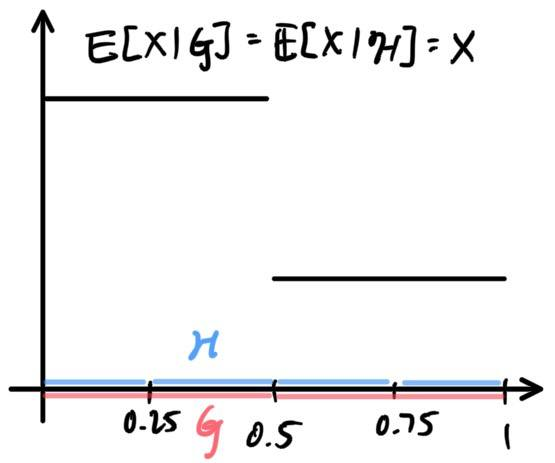
\includegraphics[scale=0.3]{img/pointless_approximation.jpg}
    \end{center}

    Then, we can see that 

      \begin{equation}
        \mathbb{E}[X \mid \mathcal{G}] = \mathbb{E}[X \mid \mathcal{H}]
      \end{equation}

    That is, the two \hyperref[prob-def:random-variable]{random variables} are exactly equal, even though $\mathcal{H}$ has more information than $\mathcal{G}$. Note that this is not the law of iterated expectations. This rule does not say that $\mathbb{E}[\mathbb{E}[X \mid \mathcal{G}]] = \mathbb{E}[ \mathbb{E}[X \mid \mathcal{H}]]$; this law is true regardless. Rather, this property is a special property of the function $X$, and therefore the Markov property is a special property of the stochastic process $\{X_t\}_{t \geq 0}$. 

\section{Poisson Processes}

  \subsection{Exponential Distribution}

    Let us do some review. The \textbf{exponential distirbution} of rate $\lambda$ is a \hyperref[prob-def:random-variable]{random variable} $T \sim \mathrm{Exponential}(\lambda)$ with CDF 

      \begin{equation}
        F_T (t) = \mathbb{P}(T \leq t) = 1 - e^{-\lambda t}
      \end{equation}

    and the PDF 

      \begin{equation}
        f_T (t) = \begin{cases} \lambda e^{-\lambda t} & t \geq 0 \\ 0 & t < 0 \end{cases}
      \end{equation}

    We have 

      \begin{equation}
        \mathbb{E}[T] = \frac{1}{\lambda}, \;\; \mathrm{Var}(T) = \frac{1}{\lambda^2}
      \end{equation}

    \begin{lemma}[Memoryless Property]
      \label{thm:memoryless-property}
      The Exp$(\lambda)$ distribution has the property that for all $t, s \geq 0$, 

        \begin{equation}
          \mathbb{P}(W > t + s \; | \; W > t) = \mathbb{P}(W > s)
        \end{equation}

      which is called the \textit{memoryless property}. We can interpret this in the following way. Let $W$ be the time you have to wait for the first arrival. Given that you already waited $t$ units of time, the probability that you have the wait $s$ additional units of time is just the probability that you wait at least $s$ from the beginning. That is, knowing that $t$ units of time have elapsed does not affect the distribution of the remaining waiting time. 
    \end{lemma}

    \begin{theorem}[Characterization of the Exponential Distribution]
      \label{thm:characterization-of-the-exponential-distribution}
      Let $W$ be a continuously distributed \hyperref[prob-def:random-variable]{random variable}. Then $W \sim$ Exp$(\lambda)$ for some $\lambda > 0$ if and only if $W$ satisfies the \hyperref[thm:memoryless-property]{memoryless property}. 
    \end{theorem}

    \begin{theorem}[Minimum of Independent Exponentials]
      \label{thm:minimum-of-independent-exponentials}
      Let $T_i \sim \mathrm{Exponential}(\lambda_i)$ for $i = 1, \ldots n$. Then, 

        \begin{equation}
          \min\{T_1, \ldots, T_n\} \sim \mathrm{Exponential}(\lambda_1 + \ldots + \lambda_n)
        \end{equation}

      and the \hyperref[prob-def:random-variable]{random variable} $I$ which takes the index of $\min\{T_1, \ldots, T_n\}$ has the PMF 

        \begin{equation}
          \mathbb{P}(I = i) = \frac{\lambda_i}{\lambda_1 + \ldots + \lambda_n}
        \end{equation}
    \end{theorem}

  \subsection{Defining the Poisson Process}

    We first describe a limiting behavior of \hyperref[prob-def:binomial-random-variable]{binomial random variables}. 

    \begin{theorem}[Poisson Limit Theorem]
      \label{thm:poisson-limit-theorem}
      Let $X_n \sim \mathrm{Bernoulli}(n, p_n)$, where $\{p_n\}_{n \in \mathbb{N}}$ is a sequence of reals in $[0, 1]$ such that 

        \begin{equation}
          \lim_{n \rightarrow \infty} n p_n = \lambda
        \end{equation}

      Letting $Y \sim \mathrm{Poisson}(\lambda)$

        \begin{equation}
          X_n \xrightarrow{D} Y
        \end{equation}

      That is, the CDFs, and since this is a discrete distribution, the PMFs, converge. 
    \end{theorem}
    \begin{proof}
      We will show that $\lim_{n \rightarrow \infty} \mathbb{P}(X_n = k) = \mathbb{P}(Y = k)$, which shows that the CDFs converge and therefore \hyperref[prob-def:convergence-in-distribution]{convergence in distribution}. 
      \begin{align*}
        \lim_{n \rightarrow \infty} \mathbb{P}(X_n = k) & = \lim_{n \rightarrow \infty} \binom{n}{k} p_n^k (1 - p_n)^k \\
        & = \lim_{n \rightarrow \infty} \frac{n (n - 1) \ldots (n - k + 1)}{k!} \bigg(\frac{\lambda}{n}\bigg)^k \bigg( 1 - \frac{\lambda}{n} \bigg)^{n - k} \\
        & = \lim_{n \rightarrow \infty} \frac{n^k + O(n^{k-1})}{k!} \frac{\lambda^k}{n^k} \bigg( 1 - \frac{\lambda}{n} \bigg)^{n - k} \\
        & = \lim_{n \rightarrow \infty} \frac{\lambda^k}{k!} \bigg( 1 - \frac{\lambda}{n} \bigg)^{n - k} \\
        & = \frac{\lambda^k}{k!} \lim_{n \rightarrow \infty} \bigg( 1 - \frac{\lambda}{n} \bigg)^n \; \lim_{n \rightarrow \infty} \bigg( 1 - \frac{\lambda}{n} \bigg)^{-k} \\
        & = \frac{\lambda^k}{k!} \, e^{\lambda} \, 1 = \frac{\lambda^k e^\lambda}{k!}
      \end{align*}
    \end{proof}

    Note that this is different from CLT because in CLT, we just assume that the $p_n$'s are constant and take the limiting behavior of $X_n \sim \mathrm{Bernoulli}(n, p)$ as $n \rightarrow \infty$. 

    This result justifies the following model. A Poisson Arrival Process with rate $\lambda > 0$ on the interval $[0, \infty)$ is a model for the occurrence of some events which may have at any time. We can interpret the process as a collection of random points in $[0, \infty)$ which are the times at which the arrivals occur. Suppose that we would like to model the arrival of events that happen completely at random at a rate $\lambda$ per unit time. At time $t = 0$, we have no arrivals yet, so $N(0) = 0$. Let us fix some $T$, and now divide $[0, T)$ into $n$ tiny subintervals of length $\delta$. 

    \begin{center}
      %\includegraphics[scale=0.3]{}
    \end{center}

    Assume that in each time slot, we assign a $X_k \sim \mathrm{Bernoulli}(\lambda \delta)$ \hyperref[prob-def:random-variable]{random variable} that determines whether there was an arrival within the interval $((k-1)\delta, k\delta]$. So with probability $\lambda\delta$, there will be an arrival within it, and as the time interval gets smaller, this probability also gets smaller too. Since every $n$ subinterval is $\mathrm{Bernoulli}(\lambda \delta)$, the number of arrivals in the interval $[0, T)$, defined as the random variable $N_n (T)$, is 

      \begin{equation}
        N_n (T) \sim \mathrm{Binomial}(n, \lambda \delta) = \mathrm{Binomial}\big(n, \frac{\lambda T}{n}\big)
      \end{equation}

    As we increase the $n$ (equivalently, decrease $\delta$), we divide $[0, T)$ into smaller and smaller subintervals, resulting in finer and finer $N_n(T)$ Binomial distributions. Since $n p_n = n \frac{\lambda T}{n} = \lambda T$ is finite, we can invoke the \hyperref[thm:poisson-limit-theorem]{Poisson limit theorem} and say 

      \begin{equation}
        N_n (T) \xrightarrow{D} \mathrm{Poisson}(\lambda T)
      \end{equation}

    Note that the starting point $0$ does not matter, and this works for any interval of length $T$. Therefore, we can model the arrival times on any interval of length $T$ as a $\mathrm{Poisson}(\lambda T)$ random variable. 

    \begin{definition}[Poisson Process]
      \label{def:poisson-process}
      Let $\lambda > 0$ be fixed, representing the rate of arrival in some unit time. The stochastic counting process $\{N(t)\}_{t \geq 0}$, where $N(t)$ represents the number of arrivals by time $t$, is called a \textbf{Poisson process} with rate $\lambda$ if 
      \begin{enumerate}
        \item $N(0) = 0$ 

        \item The number of arrivals in any interval of length $s > 0$ is $N(t + s) - N(t) \sim \mathrm{Poisson}(\lambda s)$ 

        \item $N(Tt)$ has independent increments, i.e. if $t_0 < t_1 < \ldots, < t_n$, then 

          \begin{equation}
            N(t_1) - N(t_0), \ldots, N(t_n) - N(t_{n-1})
          \end{equation}

        are independent. 
      \end{enumerate}
    \end{definition}

  \subsection{Constructing the Poisson Process}

    Now we have modeled this process using \hyperref[prob-def:random-variable]{random variables} $N(t)$ that counts the number of arrivals up to time $t$. Now, we can interpret it using random variables that represent the \textit{time} in which they arrive. 

    \begin{definition}[Arrival and Inter-Arrival Times]
      \label{def:arrival-and-inter-arrival-times}
      Set $T_0 = 0$. The arrival times are \hyperref[prob-def:random-variable]{random variables} $0 < T_1 < T_2 < T_3 < \ldots$ such that the inter-arrival waiting times

        \begin{equation}
          \tau_k = T_k - T_{k-1}, \;\;\; k \geq 0
        \end{equation}

      have the property that $\{\tau_k\}_{k=1}^\infty$ are independent $\mathrm{Exp}(\lambda)$ random variables. Define 

        \begin{equation}
          N(s) \coloneqq \max\{k \mid T_k \leq s \}
        \end{equation}
    \end{definition}

    Now we prove that this process is equivalent to the \hyperref[def:poisson-process]{Poisson process} defined before. 

    \begin{theorem}[Equivalent Interpretations]
      \label{thm:equivalent-interpretations}
      Let $\{T_n\}$ be defined as above and $N(s) \coloneqq \max\{k \mid T_k \leq s \}$. Then, 

      \begin{enumerate}
        \item $N(0) = 0$
        \item $N(s) \sim \mathrm{Poisson}(\lambda s)$ 
        \item $N(t + s) - N(t) \sim \mathrm{Poisson}(\lambda s)$ independent of $N(r)$ for $0 \leq r \leq s$. 
        \item $N(t)$ has independent incremements. 
      \end{enumerate}

      $N(s) \coloneqq \max\{k \mid T_k \leq s \}$ is a Poisson distribution with mean $\lambda s$. 
    \end{theorem}

    \begin{proof}
      From the second perspective, the statement $N(I) \sim \mathrm{Poisson}(\lambda |I|)$ for an interval $I$ means that

        \begin{equation}
          \mathbb{P}(N(I) = m) = e^{-\lambda |I|} \frac{(\lambda |I|)^m}{m!}, \qquad m = 0, 1, 2, \ldots
        \end{equation}

      where $|I|$ is the length of the interval $I$. From the first perspective, notice that

        \begin{equation}
          T_k = \tau_1 + \tau_2 + \ldots + \tau_k
        \end{equation}

      so that the $k$th arrival time $T_k$ is a sum of $k$ independent $\mathrm{Exp}(\lambda)$ \hyperref[prob-def:random-variable]{random variables}. Thus

        \begin{equation}
          T_k \sim \mathrm{Gamma}(k, \lambda)
        \end{equation}

      and therefore has density

        \begin{equation}
          \lambda e^{-\lambda t} \frac{(\lambda t)^{k-1}}{(k-1)!}, \qquad t > 0
        \end{equation}

      Note that the arrival times $T_i$ are not independent of each other, but the inter-arrival times $\tau_i$ are indeed independent.
    \end{proof}

  \subsection{The Poisson Process on a Finite Horizon}

    We can slightly modify the construction above to create a \hyperref[def:poisson-process]{Poisson process} over some finite time horizon $[0, L]$. Again, there are two equivalent ways to do this.

    \begin{enumerate}
      \item Starting with independent $\mathrm{Exp}(\lambda)$ \hyperref[prob-def:random-variable]{random variables} $\tau_1, \tau_2, \ldots$, we define

        \begin{equation}
          T_k = \sum_{i=1}^k \tau_i
        \end{equation}

      and stop once $T_k > L$.

      \item We let $N \sim \mathrm{Poisson}(\lambda L)$, since we are only working on the finite interval $[0, L]$. Given $N = n$, let $U_1, U_2, \ldots, U_n \sim \mathrm{Uniform}([0, L])$ be independent. These define the arrival times, and ordering them gives

        \begin{equation}
          T_k = U_{(k)}, \qquad k = 1, 2, \ldots, N
        \end{equation}

      where $U_{(k)}$ is the $k$th order statistic, so that $T_1 = \min(U_1, \ldots, U_N)$.
    \end{enumerate}

\section{Markov Processes}

  A Markov process is a random evolution whose future depends on its past only through
  its present. There is one definition of this, not four. The state space may be any
  measurable space $(S, \mathcal{S})$ and the time set may be any totally ordered $T$,
  with $T = \mathbb{N}$ recovering discrete time and $T = [0, \infty)$ recovering
  continuous time. Transition matrices, rate matrices, the summation form of the
  Chapman-Kolmogorov equation and the whole elementary theory of chains are
  \textit{specializations} of that one definition, and below we derive them as such
  rather than restating them.

  \subsection{Markov Kernels}

    Everything here is assembled from a single primitive: a rule assigning to each point
    of the state space a probability distribution describing where to go next.

    \begin{definition}[Markov Kernel]
      \label{def:markov-kernel}
      Let $(S, \mathcal{S})$ be a measurable space. A \textbf{Markov kernel} (also called a \textbf{transition kernel}) on $(S, \mathcal{S})$ is a map $P: S \times \mathcal{S} \rightarrow [0, 1]$ such that

      \begin{enumerate}
        \item for every $x \in S$, the set function $A \mapsto P(x, A)$ is a probability measure on $(S, \mathcal{S})$, and
        \item for every $A \in \mathcal{S}$, the map $x \mapsto P(x, A)$ is a \hyperref[mt-def:measurable-function]{measurable function}.
      \end{enumerate}

      Read $P(x, A)$ as the probability of landing in $A$ having started at $x$. Condition (1) says that each "row" of $P$ is a probability distribution. Condition (2) is what makes $P(\cdot, A)$ integrable against a measure, and it is vacuous when $S$ is countable and $\mathcal{S} = 2^S$, since every function on a countable space is measurable --- which is exactly why the elementary theory of chains never mentions it.
    \end{definition}

    A kernel acts in two directions, and holding both in view is the entire content of the
    row-vector / column-vector bookkeeping that the matrix picture forces on us.

    \begin{definition}[Action of a Kernel on Functions and on Measures]
      \label{def:action-of-a-kernel}
      Let $P$ be a \hyperref[def:markov-kernel]{Markov kernel} on $(S, \mathcal{S})$. For bounded \hyperref[mt-def:measurable-function]{measurable} $f: S \rightarrow \mathbb{R}$ define the function $P f: S \rightarrow \mathbb{R}$ by

        \begin{equation}
          (P f)(x) \coloneqq \int_S f(y) \, P(x, dy)
        \end{equation}

      and for a measure $\mu$ on $(S, \mathcal{S})$ define the measure $\mu P$ by

        \begin{equation}
          (\mu P)(A) \coloneqq \int_S P(x, A) \, \mu(dx)
        \end{equation}

      The first \textit{pulls a function backward} in time; the second \textit{pushes a measure forward} in time. Note that $P f$ is again bounded and measurable, with $\|P f\|_\infty \leq \|f\|_\infty$, and that $\mu P$ is again a probability measure whenever $\mu$ is.
    \end{definition}

    \begin{lemma}[Adjointness of the Two Kernel Actions]
      \label{thm:adjointness-of-the-two-kernel-actions}
      For every \hyperref[def:markov-kernel]{Markov kernel} $P$, every finite measure $\mu$ and every bounded measurable $f$,

        \begin{equation}
          \int_S (P f) \, d\mu = \int_S f \, d(\mu P)
        \end{equation}

      which we abbreviate as $\mu(P f) = (\mu P)(f)$.
    \end{lemma}
    \begin{proof}
      Take $f = 1_A$: the left side is $\int_S P(x, A) \, \mu(dx) = (\mu P)(A)$ by definition of $\mu P$, and the right side is $\int_S 1_A \, d(\mu P) = (\mu P)(A)$. Both sides are linear in $f$, so they agree on \hyperref[mt-def:simple-functions]{simple functions}. For bounded measurable $f$, take simple $f_k \rightarrow f$ with $\|f_k\|_\infty \leq \|f\|_\infty$ by the \hyperref[mt-thm:simple-approximation-theorem]{simple approximation theorem} and pass to the limit on both sides by the \hyperref[mt-thm:dominated-convergence-theorem]{dominated convergence theorem}.
    \end{proof}

    \begin{lemma}[Composition of Markov Kernels]
      \label{thm:composition-of-markov-kernels}
      If $P$ and $Q$ are \hyperref[def:markov-kernel]{Markov kernels} on $(S, \mathcal{S})$, then so is their \textbf{composition}

        \begin{equation}
          (P Q)(x, A) \coloneqq \int_S Q(y, A) \, P(x, dy)
        \end{equation}

      Composition agrees with composition of the induced operators, $(P Q) f = P (Q f)$, it is associative, and the kernel $I(x, A) \coloneqq 1_A (x)$ is a two-sided identity for it.
    \end{lemma}
    \begin{proof}
      For fixed $x$, $A \mapsto (P Q)(x, A)$ is a probability measure: it is nonnegative, $(PQ)(x, S) = \int_S 1 \, P(x, dy) = 1$, and countable additivity follows from \hyperref[mt-thm:monotone-convergene-theorem-mct]{monotone convergence} applied to the partial sums of $\sum_k Q(y, A_k)$ for disjoint $A_k$. For fixed $A$, $x \mapsto (PQ)(x, A)$ is measurable because it is $P$ applied to the bounded measurable function $Q(\cdot, A)$, and $P$ maps bounded measurable functions to bounded measurable functions. The identity $(PQ)f = P(Qf)$ holds for $f = 1_A$ by definition and extends to bounded measurable $f$ by linearity and dominated convergence as above; associativity and the identity law then follow from the corresponding statements for operators.
    \end{proof}

    \begin{example}[Markov Kernels on a Countable State Space]
      \label{ex:markov-kernels-on-a-countable-state-space}
      Let $S$ be countable with $\mathcal{S} = 2^S$. A \hyperref[def:markov-kernel]{Markov kernel} is then determined by the numbers $p(x, y) \coloneqq P(x, \{y\})$, since countable additivity forces $P(x, A) = \sum_{y \in A} p(x, y)$. Condition (1) of the definition says precisely

        \begin{equation}
          p(x, y) \geq 0 \quad \text{ and } \quad \sum_{y \in S} p(x, y) = 1
        \end{equation}

      that is, the matrix $\mathbf{P} = (p(x, y))_{x, y \in S}$ is \textit{row stochastic}, and condition (2) is automatic. Under this identification the two actions of the kernel become the two sides of matrix multiplication,

        \begin{equation}
          (P f)(x) = \sum_{y \in S} p(x, y) f(y) = (\mathbf{P} \mathbf{f})(x), \qquad (\mu P)(y) = \sum_{x \in S} \mu(x) p(x, y) = (\boldsymbol{\mu}^T \mathbf{P})(y)
        \end{equation}

      so $f$ is a \hyperref[lin-def:column-vector]{column vector} multiplied on the left and $\mu$ a \hyperref[lin-def:row-vector]{row vector} multiplied on the right, and \hyperref[thm:composition-of-markov-kernels]{composition of kernels} is exactly \hyperref[lin-def:matrix-multiplication]{matrix multiplication}:

        \begin{equation}
          (P Q)(x, \{z\}) = \sum_{y \in S} p(x, y) q(y, z) = (\mathbf{P} \mathbf{Q})(x, z)
        \end{equation}

      So a transition matrix is not a different object from a kernel; it is the coordinate representation of one.
    \end{example}

  \subsection{The Markov Property}

    The Markov property itself needs no kernels and no homogeneity assumption. It is a
    statement about conditional expectations, and it reads identically whether time is
    discrete or continuous.

    \begin{definition}[Markov Property]
      \label{def:markov-property}
      Let $T$ be a set with a \hyperref[st-def:total-order]{total order} (we will only use $T = \mathbb{N}$ and $T = [0, \infty)$), let $(\Omega, \mathcal{F}, \mathbb{F}, \mathbb{P})$ be a \hyperref[def:filtration]{filtered probability space} with $\mathbb{F} = (\mathcal{F}_t)_{t \in T}$, and let $(S, \mathcal{S})$ be a measurable space. A \hyperref[def:stochastic-process]{stochastic process} $\{X_t\}_{t \in T}$ taking values in $S$ and adapted to $\mathbb{F}$ satisfies the \textbf{Markov property} if for every $s \leq t$ in $T$ and every bounded \hyperref[mt-def:measurable-function]{measurable} $f: S \rightarrow \mathbb{R}$,

        \begin{equation}
          \mathbb{E}[f(X_t) \mid \mathcal{F}_s] = \mathbb{E}[f(X_t) \mid X_s] \qquad \mathbb{P}\text{-a.s.}
        \end{equation}

      Both sides are \hyperref[prob-def:random-variable]{random variables}. The content is that the best estimate of $f(X_t)$ given everything known by time $s$ is already a function of the single value $X_s$: conditioning on the whole history buys nothing beyond conditioning on the present. When no filtration is specified we always mean the \textbf{natural filtration} $\mathcal{F}_s = \sigma(X_r : r \leq s)$.
    \end{definition}

    Boundedness of $f$ is not a restriction in disguise. It is what makes every conditional
    expectation above automatically integrable; for unbounded $f$ one simply adds the
    hypothesis $\mathbb{E}|f(X_t)| < \infty$ and the same identity holds, by the same
    approximation argument used throughout this subsection.

    The elementary definition of a chain conditions on the \textit{atoms}
    $\{X_n = x_n, \ldots, X_0 = x_0\}$ and only ever looks at \textit{probabilities} rather
    than expectations. On a countable state space this is not a weaker requirement, because
    indicators generate everything.

    \begin{theorem}[The Markov Property on a Countable State Space]
      \label{thm:markov-property-on-a-countable-state-space}
      Let $S$ be countable with $\mathcal{S} = 2^S$, let $T = \mathbb{N}$, and let $(\mathcal{F}_n)$ be the natural filtration $\mathcal{F}_n = \sigma(X_0, \ldots, X_n)$. Then $\{X_n\}$ satisfies the \hyperref[def:markov-property]{Markov property} if and only if

        \begin{equation}
          \mathbb{P}(X_{n+1} = y \mid X_n = x_n, X_{n-1} = x_{n-1}, \ldots, X_0 = x_0) = \mathbb{P}(X_{n+1} = y \mid X_n = x_n)
        \end{equation}

      for every $n \geq 0$ and all $y, x_n, \ldots, x_0 \in S$ for which the conditioning event has positive probability.
    \end{theorem}
    \begin{proof}
      ($\Rightarrow$) Assume the \hyperref[def:markov-property]{Markov property}. Fix states with $\mathbb{P}(A) > 0$, where $A \coloneqq \{X_n = x_n, \ldots, X_0 = x_0\} \in \mathcal{F}_n$, and take $f = 1_{\{y\}}$. Then by the defining property of \hyperref[prob-def:cond-exp]{conditional expectation},

        \begin{align*}
          \mathbb{P}(X_{n+1} = y \mid A) & = \frac{1}{\mathbb{P}(A)} \mathbb{E}\big[ 1_A \, 1_{\{y\}}(X_{n+1}) \big] \\
          & = \frac{1}{\mathbb{P}(A)} \mathbb{E}\big[ 1_A \, \mathbb{E}[ 1_{\{y\}}(X_{n+1}) \mid \mathcal{F}_n] \big] \\
          & = \frac{1}{\mathbb{P}(A)} \mathbb{E}\big[ 1_A \, \mathbb{E}[ 1_{\{y\}}(X_{n+1}) \mid X_n] \big]
        \end{align*}

      The random variable $\mathbb{E}[1_{\{y\}}(X_{n+1}) \mid X_n]$ is $\sigma(X_n)$-measurable, hence constant on $\{X_n = x_n\}$ with value $\mathbb{P}(X_{n+1} = y \mid X_n = x_n)$, and $A \subseteq \{X_n = x_n\}$. So the last expression is $\mathbb{P}(X_{n+1} = y \mid X_n = x_n)$.

      ($\Leftarrow$) Assume the elementary identity. Since $S$ is countable, $\mathcal{F}_n$ is generated by the countably many atoms $A_{x_0 \ldots x_n} = \{X_0 = x_0, \ldots, X_n = x_n\}$, so a $\mathcal{F}_n$-measurable random variable is exactly one that is constant on each atom. Both $\mathbb{E}[1_{\{y\}}(X_{n+1}) \mid \mathcal{F}_n]$ and $\mathbb{E}[1_{\{y\}}(X_{n+1}) \mid X_n]$ are therefore constant on each atom of positive probability --- the second because $\sigma(X_n) \subseteq \mathcal{F}_n$ and each atom lies inside a single event $\{X_n = x_n\}$ --- and the hypothesis says that those two constants coincide. Hence the identity holds a.s. for $f = 1_{\{y\}}$.

      Now bootstrap in $f$. By linearity of \hyperref[prob-def:cond-exp]{conditional expectation} the identity holds for every \hyperref[mt-def:simple-functions]{simple function} $f = \sum_{i=1}^k c_i 1_{\{y_i\}}$. For bounded measurable $f$, pick simple $f_k \rightarrow f$ pointwise with $\|f_k\|_\infty \leq \|f\|_\infty$; the \hyperref[mt-thm:dominated-convergence-theorem]{dominated convergence theorem} for conditional expectation gives

        \begin{equation}
          \mathbb{E}[f_k (X_{n+1}) \mid \mathcal{G}] \longrightarrow \mathbb{E}[f(X_{n+1}) \mid \mathcal{G}] \quad \text{a.s.}
        \end{equation}

      for $\mathcal{G} = \mathcal{F}_n$ and for $\mathcal{G} = \sigma(X_n)$ alike, so the identity passes to the limit.

      Finally bootstrap in time. Suppose $\mathbb{E}[f(X_{n+m}) \mid \mathcal{F}_n] = \mathbb{E}[f(X_{n+m}) \mid X_n]$ for all bounded measurable $f$ and all $n$. Then by the tower property, for $f$ bounded measurable,

        \begin{align*}
          \mathbb{E}[f(X_{n+m+1}) \mid \mathcal{F}_n] & = \mathbb{E}\big[ \mathbb{E}[f(X_{n+m+1}) \mid \mathcal{F}_{n+1}] \mid \mathcal{F}_n \big] \\
          & = \mathbb{E}\big[ g(X_{n+1}) \mid \mathcal{F}_n \big] \\
          & = \mathbb{E}\big[ g(X_{n+1}) \mid X_n \big]
        \end{align*}

      where $g(x) \coloneqq \mathbb{E}[f(X_{n+m+1}) \mid X_{n+1} = x]$ is bounded and measurable, the second equality being the inductive hypothesis at $n+1$ and the third the one-step case just proved. Applying $\mathbb{E}[\,\cdot \mid X_n]$ to the first and last expressions of the same tower identity gives $\mathbb{E}[f(X_{n+m+1}) \mid X_n] = \mathbb{E}[g(X_{n+1}) \mid X_n]$ as well, since $\sigma(X_n) \subseteq \mathcal{F}_n$. The two left-hand sides therefore agree, which is the claim for $m+1$.
    \end{proof}

    So on a countable state space, "the expectation of every bounded measurable function"
    and "the probability of every single state" carry exactly the same information, and
    conditioning on the atoms is the same as conditioning on $\sigma(X_0, \ldots, X_n)$. The
    genuine gain in the general definition is elsewhere: it does not need
    $\mathbb{P}(X_n = x_n) > 0$, so it survives on state spaces where every singleton is
    null.

    \begin{definition}[Markov Process]
      \label{def:markov-process}
      A \hyperref[def:stochastic-process]{stochastic process} $\{X_t\}_{t \in T}$ satisfying the \hyperref[def:markov-property]{Markov property} is a \textbf{Markov process}. It is called a \textbf{discrete-time} Markov process when $T = \mathbb{N}$ and a \textbf{continuous-time} Markov process when $T = [0, \infty)$. These are the only two cases we treat, and from here on $T$ denotes one of them; every statement below written for a general $t \in T$ is a statement about both at once.
    \end{definition}

    \begin{definition}[Markov Chain]
      \label{def:markov-chain}
      A \textbf{Markov chain} is a \hyperref[def:markov-process]{Markov process} $\{X_n\}_{n \in \mathbb{N}}$ in discrete time whose state space $\mathcal{S}$ is countable (and in most examples, finite), so that every $X_n$ is a \hyperref[prob-def:discrete-random-variable]{discrete random variable}. We think of $n$ as a discrete time index, so that $X_n$ is the state of the system at time $n$ and the sequence models a system evolving randomly. By \hyperref[thm:markov-property-on-a-countable-state-space]{the countable-state characterization} the \hyperref[def:markov-property]{Markov property} is in this case equivalent to the elementary statement

        \begin{equation}
          \mathbb{P}(X_{n+1} = y \mid X_n = x_n, \ldots, X_0 = x_0) = \mathbb{P}(X_{n+1} = y \mid X_n = x_n)
        \end{equation}

      Colloquially: given that one is at state $X_n = x_n$, knowing all the previous states does not help in predicting $X_{n+1}$. Only the current state is relevant.
    \end{definition}

    In continuous time the same definition carries an extra feature worth naming now. The
    system still jumps randomly between states of $S$, but the jumps may occur at any time,
    so there are \textit{two} sources of randomness:

    \begin{enumerate}
      \item \textit{where} the system jumps, determined by the transition probabilities, and
      \item \textit{when} the system jumps, determined by the holding time.
    \end{enumerate}

    The second has no discrete-time analogue --- a discrete-time chain jumps at every tick
    --- and it is what the generator of the next subsection encodes.

  \subsection{Transition Semigroups}

    The \hyperref[def:markov-property]{Markov property} asserts that $\mathbb{E}[f(X_t) \mid \mathcal{F}_s]$ is a
    function of $X_s$, but it says nothing about \textit{which} function, nor whether that
    function depends on $s$ and $t$ separately or only on the elapsed time $t - s$. Pinning
    this down is a second, independent assumption, and it is where kernels enter.

    \begin{definition}[Transition Semigroup]
      \label{def:transition-semigroup}
      A \hyperref[def:markov-process]{Markov process} $\{X_t\}_{t \in T}$ is \textbf{time-homogeneous with transition semigroup} $(P_t)_{t \in T}$ if each $P_t$ is a \hyperref[def:markov-kernel]{Markov kernel} on $(S, \mathcal{S})$ and, for every $s, t \in T$ and every bounded measurable $f$,

        \begin{equation}
          \mathbb{E}[f(X_{s + t}) \mid \mathcal{F}_s] = \mathbb{E}[f(X_{s + t}) \mid X_s] = (P_t f)(X_s)
        \end{equation}

      Note that $P_t$ carries no $s$: the operator depends only on the elapsed time $t$, which is exactly the assertion that the process is \textbf{time-homogeneous}. The family $(P_t)_{t \in T}$ is required to satisfy

      \begin{enumerate}
        \item $P_0 = I$, the identity kernel, and
        \item the \textbf{Chapman-Kolmogorov equation} $P_{s + t} = P_s P_t$ for all $s, t \in T$,
      \end{enumerate}

      which make $(P_t)_{t \in T}$ a \hyperref[alg-def:semigroup]{semigroup} of operators under \hyperref[thm:composition-of-markov-kernels]{kernel composition} --- a monoid homomorphism from $(T, +)$ into the kernels on $(S, \mathcal{S})$.
    \end{definition}

    Two readings of $P_t$ are available, by \hyperref[def:action-of-a-kernel]{the two actions of a kernel},
    and both get used constantly:

    \begin{enumerate}
      \item $P_t$ \textit{pushes the measure forward}: if $X_s \sim \rho_s$ then $X_{s+t} \sim \rho_s P_t$, so $\rho_{s+t} = \rho_s P_t$. In coordinates this is $\boldsymbol{\rho_{s+t}}^T = \boldsymbol{\rho_s}^T \mathbf{P_t}$.

      \item $P_t$ \textit{pulls the function back}: it sends the function $f$ evaluated at time $s + t$ to the function $P_t f$ evaluated at time $s$. In coordinates this is $\mathbf{f} \mapsto \mathbf{P_t} \mathbf{f}$.
    \end{enumerate}

    These are the same statement, by \hyperref[thm:adjointness-of-the-two-kernel-actions]{adjointness}: whether we compute $(\boldsymbol{\rho_s}^T \mathbf{P_t}) \mathbf{f}$ or $\boldsymbol{\rho_s}^T (\mathbf{P_t} \mathbf{f})$, we get $\mathbb{E}[f(X_{s+t})]$. Spelled out,

      \begin{equation}
        \mathbb{E}[f(X_{s + t})] = \mathbb{E}\big[ \mathbb{E}[f(X_{s+t}) \mid X_s] \big] = \mathbb{E}[(P_t f)(X_s)] = \int_S P_t f \, d\rho_s = \int_S f \, d\rho_{s+t}
      \end{equation}

    so $P_t$ lets us compute anything about the distribution of $X_{s+t}$ from the distribution of $X_s$, which we know.

    \begin{lemma}[Chapman-Kolmogorov Equation]
      \label{thm:chapman-kolmogorov-equation}
      The semigroup law $P_{s + t} = P_s P_t$ is forced by the \hyperref[def:markov-property]{Markov property}; it is not an extra assumption on top of homogeneity. In terms of \hyperref[def:transition-probability]{transition probabilities} it reads

        \begin{equation}
          p_{s + t}(x, A) = \int_S p_t (y, A) \, p_s (x, dy)
        \end{equation}
    \end{lemma}
    \begin{proof}
      Let $f$ be bounded measurable and $r \in T$. Using the tower property and then the \hyperref[def:markov-property]{Markov property} twice,

        \begin{align*}
          (P_{s + t} f)(X_r) & = \mathbb{E}[ f(X_{r + s + t}) \mid X_r] \\
          & = \mathbb{E}\big[ \mathbb{E}[ f(X_{r + s + t}) \mid \mathcal{F}_{r + s}] \mid \mathcal{F}_r \big] \\
          & = \mathbb{E}\big[ (P_t f)(X_{r + s}) \mid \mathcal{F}_r \big] \\
          & = (P_s (P_t f))(X_r)
        \end{align*}

      since $P_t f$ is itself bounded and measurable. The displayed integral form is this identity applied to $f = 1_A$, using \hyperref[thm:composition-of-markov-kernels]{composition of kernels}.
    \end{proof}

    \begin{lemma}[Linearity of the Transition Operator]
      \label{thm:linearity-of-the-transition-operator}
      Each $P_t$ is a linear operator: for $\alpha, \beta \in \mathbb{R}$ and bounded \hyperref[mt-def:measurable-function]{measurable functions} $f, g$,

        \begin{equation}
          P_t (\alpha f + \beta g) = \alpha P_t f + \beta P_t g
        \end{equation}
    \end{lemma}
    \begin{proof}
      By linearity of \hyperref[prob-def:cond-exp]{conditional expectation},

        \begin{align*}
          (P_t (\alpha f + \beta g))(X_s) & = \mathbb{E}[(\alpha f + \beta g)(X_{s + t}) \mid X_s] \\
          & = \mathbb{E}[(\alpha f)(X_{s + t}) \mid X_s] + \mathbb{E}[(\beta g)(X_{s + t}) \mid X_s] \\
          & = \alpha (P_t f)(X_s) + \beta (P_t g)(X_s)
        \end{align*}
    \end{proof}

    \begin{lemma}[Conservativeness]
      \label{thm:conservativeness}
      $P_t 1 = 1$ for every $t \in T$, where $1 = 1_S$ is the constant function $1$.
    \end{lemma}
    \begin{proof}
      Immediate from $P_t(x, \cdot)$ being a probability measure: $(P_t 1)(x) = P_t(x, S) = 1$. Probabilistically this is the \hyperref[prob-thm:law-of-total-probability]{law of total probability}, since $(P_t 1_S)(X_s) = \mathbb{E}[1_S (X_{s+t}) \mid X_s] = 1$.
    \end{proof}

    Specializing $f$ to an indicator recovers the familiar probabilistic language.

    \begin{definition}[Transition Probability]
      \label{def:transition-probability}
      For a Markov process with \hyperref[def:transition-semigroup]{transition semigroup} $(P_t)$, the \textbf{transition probability} (or \textbf{transition function}) is

        \begin{equation}
          p_t (x, A) \coloneqq (P_t 1_A)(x) = \mathbb{E}[1_A (X_{s + t}) \mid X_s = x] = \mathbb{P}(X_{s + t} \in A \mid X_s = x)
        \end{equation}

      which is nothing but the kernel $P_t$ written as a set function; conditions (1) and (2) of \hyperref[def:markov-kernel]{the kernel definition} say respectively that $A \mapsto p_t(x, A)$ is a probability measure and that $x \mapsto p_t(x, A)$ is measurable. When $p_t(x, \cdot)$ is \hyperref[mt-def:absolutely-continuous-measures]{absolutely continuous} with density $p_t(x, \cdot)$ we write

        \begin{equation}
          p_t(x, A) = \int_A p_t(x, y) \, dy
        \end{equation}

      overloading the symbol in the customary way.
    \end{definition}

    We can now collect the specializations. The first says that in discrete time the whole
    semigroup is generated by a single kernel, so "the transition matrix" really is the only
    datum.

    \begin{theorem}[Discrete Time: the Semigroup Is Generated by One Kernel]
      \label{thm:discrete-time-semigroup-is-generated-by-one-kernel}
      Let $T = \mathbb{N}$ and write $P \coloneqq P_1$. Then $P_n = P^n$ for every $n \in \mathbb{N}$, and conversely every \hyperref[def:markov-kernel]{Markov kernel} $P$ determines a \hyperref[def:transition-semigroup]{transition semigroup} by $P_n \coloneqq P^n$.
    \end{theorem}
    \begin{proof}
      Induct on $n$. The case $n = 0$ is $P_0 = I = P^0$ and the case $n = 1$ holds by definition. If $P_n = P^n$, then \hyperref[thm:chapman-kolmogorov-equation]{Chapman-Kolmogorov} gives $P_{n+1} = P_n P_1 = P^n P = P^{n+1}$. For the converse, $P^n$ is a Markov kernel by \hyperref[thm:composition-of-markov-kernels]{closure of kernels under composition}, and $P^{m+n} = P^m P^n$ is just associativity.
    \end{proof}

    In continuous time no such single generating kernel exists --- there is no "smallest
    positive time" --- and its role is played instead by the infinitesimal generator of the
    next subsection.

    \begin{definition}[Transition Matrix]
      \label{def:transition-matrix}
      Let $S$ be countable and $T = \mathbb{N}$. By \hyperref[ex:markov-kernels-on-a-countable-state-space]{the countable-state description of kernels} the one-step kernel $P = P_1$ is the row-stochastic matrix

        \begin{equation}
          P_{x y} = P(x, y) = \mathbb{P}(X_1 = y \mid X_0 = x) = \mathbb{P}(X_{n+1} = y \mid X_n = x)
        \end{equation}

      called the \textbf{transition probability matrix}, the probability of moving from $x$ to $y$ in one step. The last equality is time-homogeneity: the one-step probabilities do not change with $n$. If $\mathcal{S}$ is finite then $P$ is a $|\mathcal{S}| \times |\mathcal{S}|$ matrix, and if $\mathcal{S}$ is countably infinite it is an infinite matrix. By \hyperref[thm:discrete-time-semigroup-is-generated-by-one-kernel]{the previous theorem} the $m$-step probabilities are then the matrix powers,

        \begin{equation}
          \mathbb{P}(X_{n + m} = y \mid X_n = x) = p_m(x, y) = \mathbf{P}^m (x, y)
        \end{equation}

      and \hyperref[thm:conservativeness]{conservativeness} $\mathbf{P} \mathbf{1} = \mathbf{1}$ is exactly the statement that $\mathbf{P}$ is stochastic.
    \end{definition}

  \begin{example}[Transition Operator as a Matrix in Discrete Space]
    \label{ex:transition-operator-as-a-matrix-in-discrete}
    Let us have a discrete space $S = \{1, \ldots, d\}$ with indicators $1_{\{i\}}$ for $i = 1, \ldots, d$, and let $\boldsymbol{\rho_s}$ be the \hyperref[lin-def:column-vector]{column vector} holding the PMF of $X_s$. Taking $f = 1_{\{j\}}$ lets us compute the probability of $X_{s + t}$ landing at each point $j \in S$, which is what we care about for discrete distributions. This works verbatim for $T = \mathbb{N}$ and for $T = [0, \infty)$; only the admissible values of $t$ differ. 

    \begin{align*}
      \boldsymbol{\rho_{s + t}} (j) & = \mathbb{P}( X_{s + t} = j) \\ 
      & = \mathbb{E}[1_{\{j\}} (X_{s + t})] \\
      & = \mathbb{E} [ \mathbb{E}[ 1_{\{j\}} (X_{s + t}) \mid X_s] ] && = \mathbb{E}[P_t 1_{\{j\}} (X_s)] \\
      & = \int_S \mathbb{E}[ 1_{\{j\}} (X_{s + t}) \mid X_s] d\rho_s && = \int_S P_t 1_{\{j\}} (X_s) \,d \rho_s \\
      & = \sum_{i \in S} \mathbb{P}[ X_{s + t} = j \mid X_s = i] \, \mathbb{P} ( X_s = i) && = \sum_{i \in S} P_t 1_{\{j\}} (i) \mathbb{P}(X_s = i) 
    \end{align*}

    which can be summarized as 

      \begin{equation}
        \boldsymbol{\rho_{s + t}} (j) = \sum_{i = 1}^d P_t 1_{\{j\}} (i) \boldsymbol{\rho_s} (i) = \sum_{i = 1}^d \mathbb{P}(X_{s + t} = j \mid X_s = i) \, \boldsymbol{\rho_s} (i)
      \end{equation}

    We can compactly organize the probabilities of these internode travel inside a $d \times d$ right stochastic \textbf{\hyperref[def:transition-matrix]{transition matrix}}

      \begin{equation}
        \mathbf{P_t} = \begin{pmatrix} P_t 1_{\{1\}} (1) & \ldots & P_t 1_{\{d\}} (1) \\ \vdots & \ddots & \vdots \\ P_t 1_{\{1\}} (d) & \ldots & P_t 1_{\{d\}} (d) \end{pmatrix} = \begin{pmatrix} \mathbb{P}(X_{s + t} = 1 \mid X_s = 1) & \ldots & \mathbb{P}(X_{s + t} = d \mid X_s = 1) \\ \vdots & \ddots & \vdots \\ \mathbb{P}(X_{s + t} = 1 \mid X_s = d) & \ldots & \mathbb{P}(X_{s + t} = d \mid X_s = d) \end{pmatrix}
      \end{equation}

    and compactly write the above equation as 

      \begin{equation}
        \boldsymbol{\rho_{s + t}}^T = \boldsymbol{\rho_{t}}^T \mathbf{P_t}
      \end{equation}
  \end{example}

  \begin{example}[Markov Property in Discrete Space]
    \label{ex:markov-property-in-discrete-space}
    If we wanted to extract information from $X_s$ with function $f$ (i.e. compute $\mathbb{E}[f(X_s)]$), we can calculate 

      \begin{equation}
        \mathbb{E}[f(X_s)] = \boldsymbol{\rho_s}^T \mathbf{f} =  \begin{pmatrix} \boldsymbol{\rho_s} (1) & \ldots & \boldsymbol{\rho_s} (d) \end{pmatrix} \begin{pmatrix} f_1 \\ \vdots \\ f_d \end{pmatrix}
      \end{equation}
       

    Now, say that $s$ units of time later, we want to extract information $f$ from $X_{s + t}$ by computing 

      \begin{equation}
        \mathbb{E}[f(X_{s + t})] = \boldsymbol{\rho_{s + t}}^T \mathbf{f} = \begin{pmatrix} \boldsymbol{\rho_{s + t}} (1) & \ldots &  \boldsymbol{\rho_{s + t}} (d) \end{pmatrix} \begin{pmatrix} f_1 \\ \vdots \\ f_d \end{pmatrix}
      \end{equation}

    The problem is that we don't know what the distribution of $X_{s + t}$ is (i.e. don't know $\boldsymbol{\rho_{s + t}} (i)$), so we get its expectation by conditioning it on $X_s$, which realizes as taking the expectation of a \textit{different} function $P_t f$ with respect to $\rho_s$. 

      \begin{equation}
        \mathbb{E}[f(X_{s + t})] = \mathbb{E}[ \mathbb{E}[ f(X_{s + t}) \mid X_s]] = \mathbb{E}[(P_t f)(X_s)] = \begin{pmatrix} \boldsymbol{\rho_s} (1) & \ldots & \boldsymbol{\rho_s} (d) \end{pmatrix} \begin{pmatrix} (P_t f)_1 \\ \vdots \\(P_t f)_d \end{pmatrix}
      \end{equation}

    It turns out that this transformation $\mathbf{f} \mapsto \mathbf{P_t} \mathbf{f}$ (from \hyperref[lin-def:row-vector]{row vector} to row vector) is linear, and so we can interpret $\mathbf{P_t}$ as $\mathbf{f}$ that has been left-multiplied by some transformation matrix $\mathbf{P_t}$. 

      \begin{equation}
        \begin{pmatrix} \boldsymbol{\rho_s} (1) & \ldots & \boldsymbol{\rho_s} (d) \end{pmatrix} \begin{pmatrix} (P_t f)_1 \\ \vdots \\(P_t f)_d \end{pmatrix} = \begin{pmatrix} \boldsymbol{\rho_s} (1) & \ldots & \boldsymbol{\rho_s} (d) \end{pmatrix} \underbrace{\begin{pmatrix} && \\ & \mathbf{P_t} & \\ && \end{pmatrix} \begin{pmatrix} f_1 \\ \vdots \\ f_d \end{pmatrix}}_{\mathbf{P_t f}}
      \end{equation}

    It turns out that this $\mathbf{P_t}$ acts linearly on $\mathbf{f}$ through left multiplication, but we can also right-multiply $\boldsymbol{\rho_s}$ by $\mathbf{P_t}$ to get the new distribution of $X_{s + t}$! 

      \begin{equation}
        \begin{pmatrix} \boldsymbol{\rho_s} (1) & \ldots & \boldsymbol{\rho_s} (d) \end{pmatrix} \begin{pmatrix} (P_t f)_1 \\ \vdots \\(P_t f)_d \end{pmatrix} = \underbrace{\begin{pmatrix} \boldsymbol{\rho_s} (1) & \ldots & \boldsymbol{\rho_s} (d) \end{pmatrix} \begin{pmatrix} && \\ & \mathbf{P_t} & \\ && \end{pmatrix}}_{\boldsymbol{\rho_s}^T \mathbf{P_t} = \boldsymbol{\rho_{s + t}}^T} \begin{pmatrix} f_1 \\ \vdots \\ f_d \end{pmatrix}
      \end{equation}

    Therefore, it turns out that the linearity of $\mathbf{P_t}$ on $\mathbf{f}$ implies linearity of it on the vector $\boldsymbol{\rho_s}$. 
  \end{example}

    \begin{example}[Chapman-Kolmogorov in Discrete Space]
      \label{ex:chapman-kolmogorov-in-discrete-space}
      Setting $x = i$ and $A = \{j\}$ in \hyperref[thm:chapman-kolmogorov-equation]{Chapman-Kolmogorov} and replacing the integral by a sum,

      \begin{align}
        \mathbf{P_{s + t}} (i, j) & = p_{s + t} (i, \{j\}) \\
                                  & = \int_S p_t (y, \{j\}) \, p_s (i, dy) \\
                                  & = \sum_{y \in S} p_s (i, \{y\}) \, p_t (y, \{j\}) \\
                                  & = \sum_{y \in S} \mathbf{P_s} (i, y) \, \mathbf{P_t} (y, j)
      \end{align}

      so $\mathbf{P_{s + t}} = \mathbf{P_s} \mathbf{P_t}$: conditioning on the intermediate node is matrix multiplication. In discrete time, taking $t = 1$ recovers $\mathbf{P_{m+1}} = \mathbf{P_m} \mathbf{P}$ and hence $\mathbf{P_m} = \mathbf{P}^m$ once more.
    \end{example}

  \begin{example}[Transition Matrix from the Semigroup]
    \label{ex:transition-matrix-from-the-semigroup}
  Given the transition matrix 
  \begin{equation}
    \mathbf{P_t} = \begin{pmatrix} P_t 1_{\{1\}} (1) & \ldots & P_t 1_{\{d\}} (1) \\ \vdots & \ddots & \vdots \\ P_t 1_{\{1\}} (d) & \ldots & P_t 1_{\{d\}} (d) \end{pmatrix}
  \end{equation}
  note that by linearity of $P_t$ and the fact that $\{j\}$ forms a partition of $S$, we have a
  \begin{equation}
    \sum_{j \in S} (P_t 1_{\{j\}}) (i) = \bigg[ P_t \bigg( \sum_{j \in S} 1_{\{j\}} \bigg) \bigg] \big( i \big) = (P_t 1_S) (i) = 1_S (i) = 1
  \end{equation}
  which means that each row must sum to $1$, i.e. that $\mathbf{P_t}$ is row stochastic --- which is \hyperref[thm:conservativeness]{conservativeness} written out in coordinates. 
  \end{example}

  \subsection{Generators}

    In discrete time \hyperref[thm:discrete-time-semigroup-is-generated-by-one-kernel]{the whole semigroup is $P_n = P^n$}, so the single kernel $P$ determines everything, and the natural "rate of change per unit time" is simply the difference operator

      \begin{equation}
        \mathscr{L} \coloneqq P - I
      \end{equation}

    In continuous time there is no smallest positive time step and hence no generating kernel, so its role is taken over by the right derivative of $P_t$ at $t = 0$. The two are the same construction: $\mathscr{L} = \lim_{t \downarrow 0} (P_t - I)/t$ reduces to $P - I$ when the only available $t$ is $t = 1$. Everything below is stated for continuous time, where the limit has content.


    In the discrete time case, we had $P_t = (p_1)^t$ for $t \in \mathbb{N}$, and from the \hyperref[thm:chapman-kolmogorov-equation]{Chapman-Kolmogorov equation}, knowing $p_1$ allows us to compute $p_t$ for all $t \in \mathbb{N}$. Likewise, if we know the \hyperref[def:transition-probability]{transition probability} for some $t < t_0$ for any $t_0 > 0$, we know it for all $t$. This observation suggests that the transition probabilities $p_t$ can be determined from their derivatives at $0$. 

    We now define the analogous operator to the transition rate matrix in continuous-time chains with a finite state space. This is a natural extension, since we are just taking the right-derivative of $P_t$ at $t = 0$. 

    \begin{definition}[Generator]
      \label{def:generator}
    The generator $\mathscr{L}$ is defined as 
    \begin{equation}
      \mathscr{L} f \coloneqq \lim_{t \downarrow 0} \frac{P_t f - f}{t}
    \end{equation}
    for every $f \in L^2 (\mu)$ for which the above limit exists in $L^2 (\mu)$. Intuitively, $\mathscr{L} f$ represents the instantaneous rate of change of the measurement $f$. The set of $f$ for which $\mathscr{L}f$ is defined is called the domain $\mathrm{Dom}(\mathscr{L})$ of the generator, and $\mathscr{L}$ defines a linear operator from $\mathrm{Dom}(\mathscr{L}) \subset L^2 (\mu)$ to $L^2 (\mu)$. 
    \end{definition}

    We have defined the generator $\mathscr{L}$ from the Markov \hyperref[alg-def:semigroup]{semigroup} $\{P_t\}_{t \geq 0}$. Now, let's try to define the semigroup in terms of the generator $\mathscr{L}$. Given that we have some map $\mathscr{L}$, can we define some semigroup $\{P_t\}$ satisfying the definition? We know that by the semigroup property, we can split $P_{t + h}$ into $P_t P_h$ and $P_h P_t$, from which we get the \textbf{Kolmogorov backward equation} and the \textbf{forward equation}, respectively. 
    \begin{align*}
        \frac{d}{dt} P_t & = \lim_{h \downarrow 0} \frac{P_{t + h} - P_t}{h} = \lim_{h \downarrow 0} \frac{P_t ( P_h - I)}{h} = P_t \bigg( \lim_{h \downarrow 0} \frac{P_h - I}{h} \bigg) = P_t \mathscr{L} \\
        \frac{d}{dt} P_t & = \lim_{h \downarrow 0} \frac{P_{t + h} - P_t}{h} = \lim_{h \downarrow 0} \frac{( P_h - I) P_t}{h} = \bigg( \lim_{h \downarrow 0} \frac{P_h - I}{h} \bigg) P_t = \mathscr{L} P_t
    \end{align*}
    From which we see that the generator $\mathscr{L}$ commutes with the semigroup 
    \begin{equation}
      \mathscr{L} P_t = P_t \mathscr{L}
    \end{equation}
    and solving this differential equation gives 
    \begin{equation}
      P_t = e^{t \mathscr{L}}
    \end{equation}

    Let's observe how this generator acts on the indicator functions $f = 1_A$. Note that $P_s 1_A (i) = \mathbb{P}(X_{t + s} \in A \mid X_t = i)$. 
    \begin{equation}
      (\mathscr{L} 1_A) (i) = \bigg( \lim_{h \downarrow 0} \frac{P_h 1_A - 1_A}{h} \bigg) (i) = \lim_{h \downarrow 0} \frac{ P_h 1_A (i) - 1_A (i)}{h}
    \end{equation}
    and so $(\mathscr{L} 1_A)(i)$ represents the infinitesimal rate of change of the probability that $X_t$ will be in $A$ given that it is at $1$. 

    Now, how does the generator realize into the finite state space? 

    \begin{example}[Transition Rate Matrix]
      \label{ex:transition-rate-matrix}
      We know that the \hyperref[alg-def:semigroup]{semigroup} operator $P_t$ is equivalent to the \hyperref[def:transition-matrix]{transition matrix} 

        \begin{equation}
          \mathbf{P_t} = \begin{pmatrix} P_t (1, 1) & \ldots & P_t (1, d) \\ \vdots & \ddots & \vdots \\ P_t (d, 1) & \ldots & P_t (d, d) \end{pmatrix}
        \end{equation}

      Let's say that we have the function $f = \sum_{i \in S} c_i 1_{\{i\}}$, which realizes as the function vector $\mathbf{f}$, and we have generator $\mathscr{L}$. We know that $P_t f$ realizes as the \hyperref[lin-def:matrix-multiplication]{matrix multiplication} $\mathbf{P_t} \mathbf{f}$, and so we can define the \textbf{transition rate matrix} $\mathbf{Q}$ satisfying the equation 

        \begin{equation}
          \mathbf{Q} \mathbf{f}= \lim_{h \rightarrow 0} \frac{\mathbf{P_h} \mathbf{f} - \mathbf{f}}{h} \implies \mathbf{Q} = \lim_{h \rightarrow 0} \frac{\mathbf{P_h} - \mathbf{I}}{h}
        \end{equation}

      This derivatives has entries 

        \begin{align}
          Q(i, j) = \frac{d}{dt} \bigg|_{t = 0} \mathbf{P_t} (i, j) = \lim_{h \rightarrow 0} \frac{\mathbf{P_h} (i, j) - \mathbf{P_0} (i, j)}{h} = \begin{dcases} \lim_{h \rightarrow 0} \frac{P_h (i, j)}{h} & \text{ if } i \neq j \\ \lim_{h \rightarrow 0} \frac{P_h (i, i) - 1}{h} & \text{ if } i = j \end{dcases}
        \end{align}

      representing the flow of probability from $i \mapsto j$. Note that by the \hyperref[prob-thm:law-of-total-probability]{law of total probability}, 

        \begin{equation}
          \sum_j \mathbf{P_t} (i, j) = 1 \implies \frac{d}{dt} \bigg|_{t = 0} \sum_{j} \mathbf{P_t} (i, j) =  \sum_j \frac{d}{dt} \bigg|_{t = 0} \mathbf{P_t} (i, j) = \sum_{j} \mathbf{Q} (i, j) = 0
        \end{equation}

      So the diagonal entries is simply $\mathbf{Q}(i, i) = - \sum_{j \neq i} Q(i, j)$. This realization $\mathbf{Q}$ is consistent with the way $\mathscr{L}$ operates. Given $f = \sum_i f_i 1_{\{i\}}$, and not worrying about whether we evaluate a limit of functions or the limit of evaluations, we can get 

      \begin{align*}
        (\mathscr{L} f) (i) & = \bigg[ \mathscr{L} \bigg( \sum_{j=1}^d f_j 1_{\{j\}} \bigg) \bigg] (i) = \bigg( \sum_{j=1}^d f_j \mathscr{L} 1_{\{j\}} \bigg) (i) = \sum_{j=1}^d f_j ( \mathscr{L} 1_{\{j\}}) (i) \\ 
        & = \sum_{j=1}^d f_j \bigg( \lim_{h \downarrow 0} \frac{P_h 1_{\{ j\}} (i) - 1_{\{j\}} (i)}{h} \bigg) = \sum_{j=1}^d f_j \bigg( \lim_{h \downarrow 0} \frac{\mathbf{P_h} (i, j) - \mathbf{P_0} (i, j)}{h} \bigg) \\
        & = \sum_{j=1}^d \mathbf{Q}(i, j) f_j = (\mathbf{Q} \mathbf{f})_i 
      \end{align*}

      and therefore, setting $f = 1_{\{j\}}$, we get 

        \begin{equation}
          \mathscr{L} 1_{\{j\}} (i) = Q(j, i)
        \end{equation}
    \end{example}

    \begin{example}[Two-State Continuous-Time Chain]
      \label{ex:two-state-continuous-time-chain}
      Given a two-state \hyperref[def:markov-chain]{Markov chain}, $\{0, 1\}$, with some $\lambda \geq 0$. Then, we can model our \hyperref[def:transition-probability]{transition probability} matrix as 

        \begin{equation}
          P_s  = \begin{pmatrix} \frac{1}{2} + \frac{1}{2} e^{-2\lambda t} &  \frac{1}{2} - \frac{1}{2} e^{-2\lambda t} \\  \frac{1}{2} - \frac{1}{2} e^{-2\lambda t} &  \frac{1}{2} + \frac{1}{2} e^{-2\lambda t} \end{pmatrix}
        \end{equation}

      Its generator matrix is 

        \begin{equation}
          Q = \begin{pmatrix} -\lambda & \lambda \\ \lambda & -\lambda \end{pmatrix}
        \end{equation}
    \end{example}

  \subsection{Chains on a Countable State Space}

    Everything in this subsection is the specialization $S$ countable, $T = \mathbb{N}$. The chain is described by its \hyperref[def:transition-matrix]{transition matrix} $\mathbf{P}$, and by \hyperref[thm:markov-property-on-a-countable-state-space]{the countable-state characterization} we may work directly with elementary conditional probabilities.
  \begin{definition}[Absorbing State]
    \label{def:absorbing-state}
    A state $F$ in the state space $\mathcal{S}$ of a \hyperref[def:markov-chain]{Markov chain} is called an \textbf{absorbing state} if
    \begin{equation}
      \mathbb{P}(X_{n+1} = F \; | \; X_n = F) = 1 \iff \mathbb{P}(X_{n+1} \neq F \; | \; X_n = F) = 0
    \end{equation}
  \end{definition}

  \begin{theorem}[Finite-Dimensional Distributions of a Markov Chain]
    \label{thm:finite-dimensional-distributions-of-a-markov}
    Let there exist a time homogeneous \hyperref[def:markov-chain]{Markov chain} with transition probability matrix $P$. Given a probability distribution $\nu_n$ (a \hyperref[lin-def:row-vector]{row vector}) representing the a state of a system at time $t=n$, the probability distribution of which state the system will be at when $t=n+1$ can be calculated by 
    \begin{equation}
      \nu_{n+1} = \nu_n P
    \end{equation}
    The probability distribution of the state of the system at $t=n+k$ can be calculated by summing up all of the possible probabilities that lead to each state at $t=n+k$. It is calculated equivalently as \hyperref[lin-def:matrix-multiplication]{matrix multiplication}: 
    \begin{equation}
      \nu_{n+k} = \nu_n P^k
    \end{equation}
  \end{theorem}

  \begin{definition}[Initial Distribution]
    \label{def:initial-distribution}
    The distribution $\nu$ of a \hyperref[def:markov-chain]{Markov chain} at time $t=0$ is called the \textit{initial distribution} for the chain. That is, $\nu$ is the initial distribution if 
    \begin{equation}
      \mathbb{P}(X_0 = x) = \nu(x)
    \end{equation}
  \end{definition}

  \begin{definition}[Stationary Distribution]
    \label{def:stationary-distribution}
    An \textit{invariant distribution}, or \textit{stationary distribution}, is a probability distribution $\pi$ such that 
    \begin{equation}
      \pi P = \pi
    \end{equation}
    This means that 
    \begin{equation}
      \pi P^k = \pi
    \end{equation}
    for all $k \in \mathbb{N}$. We can equivalently call $\pi$ the left eigenvector of matrix $P$ with eigenvalue $1$. If $\pi$ is an invariant distribution for the chain, and $X_0 \sim \pi$, then the distribution of $X_n$ does not change with $n$; it is invariant. Note that this does not mean that $X_n$ is constant; rather, it means that the distribution of $X_n$ is not changing. 
  \end{definition}

  \begin{example}[A Two-State Chain]
    \label{ex:a-two-state-chain}
    Let us have a two node system with nodes labeled $L$ and $R$. That is, $\mathcal{S} = \{L, R\}$. Consider a chain on this state space with transition probability matrix. 
    \begin{equation}
      P = \begin{pmatrix}
      1-a & a \\ b & 1-b 
      \end{pmatrix}
    \end{equation}
    which can be visualized in the following diagram below.
    \begin{center}
    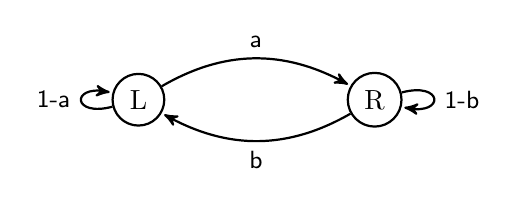
\begin{tikzpicture}[->,>=stealth',shorten >=1pt,auto,node distance=3cm,
                        thick,main node/.style={circle,draw}]
        \node[main node] (R) {R};
        \node[main node] (L) [left of=R] {L};
        \path[every node/.style={font=\sffamily\small}]
        (L) edge [loop left] node {1-a} (L)
            edge [bend left] node {a} (R)
        (R) edge [loop right] node {1-b} (R)
            edge [bend left] node {b} (L);
    \end{tikzpicture}
    \end{center}

    Then, the \hyperref[def:stationary-distribution]{stationary distribution} is 
    \begin{equation}
      \pi = \Big( \frac{b}{a+b}, \frac{a}{a+b} \Big)
    \end{equation}
    Notice that if $a = b = 0$, then this definition is ill-defined, and any probability distribution is invariant since $P = I_2$, the identity matrix. 
  \end{example}

  \begin{definition}[Recurrent]
    \label{def:recurrent}
    A state $x \in \mathcal{S}$ is \textit{recurrent} if
    \begin{equation}
      \mathbb{P}(X_n = x \text{ for some } n \geq 1 \, | \, X_0 = x) = 1
    \end{equation}
    That is, if the initial state is $x$, the chain has probability $1$ of returning to $x$ at some later time. If a state is not recurrent, then the state is said to be \textit{transient}. That is, if $x$ is transient, there is some positive probability that the chain will never return to $x$. 
  \end{definition}


  \begin{definition}[Irreducible Chains]
    \label{def:irreducible-chains}
    If all pairs $x, y \in \mathcal{S}$ communicate, then the chain is said to be \textit{irreducible}. If there exists a pair of states that do not communicate, then the chain is said to be \textit{reducible}. 
  \end{definition}

  Note that the notion of communication is an \hyperref[st-def:equivalence_relation]{equivalence relation} between states. That is, it satisfies the properties. 
  \begin{enumerate}
    \item $x \leftrightarrow x$.
    \item $x \leftrightarrow y \implies y \leftrightarrow x$.
    \item $x \leftrightarrow y, y \leftrightarrow z \implies x \leftrightarrow z$.
  \end{enumerate}
  This relation partitions the state space $\mathcal{S}$ uniquely into transient states and irreducible sub-chains
  \begin{equation}
    \mathcal{S} = T \cup C_1 \cup C_2 \cup ...
  \end{equation}
  More specifically, $T$ is the set of all transient states, and the sets $C_k$ are \textit{closed communication classes}, meaning that
  \begin{enumerate}
    \item For all $x, y \in C_k$, $x \leftrightarrow y$. 
    \item $P(x, z) = 0$ whenever $x \in C_k$ but $z \not\in C_k$. 
  \end{enumerate}
  Note that for all $x, y \not\in T$, $x$ and $y$ communicate if and only if $x$ and $y$ are in the same class $C_k$. Moreover, once the chain reaches one of the sets $C_k$, it cannot leave $C_k$. 




  \begin{theorem}[Unique Stationary Distribution for a Finite Irreducible Chain]
    \label{thm:unique-stationary-distribution-for-a-finite}
    Suppose $|\mathcal{S}| < \infty$. If the chain is irreducible, then there always exists a unique \hyperref[def:stationary-distribution]{stationary distribution} $\pi$. If the chain is also aperiodic, then for any \hyperref[def:initial-distribution]{initial distribution} $\nu$, 
    \begin{equation}
      \lim_{k \rightarrow \infty} \nu P^k = \pi
    \end{equation}
    Hence
    \begin{equation}
      \lim_{k \rightarrow \infty} P^{(k)}(x, y) = \pi(y)
    \end{equation}
    for all $x, y \in \mathcal{S}$. Furthermore, for any function $F: \mathcal{S} \to \mathbb{R}$, the limit
    \begin{equation}
      \lim_{N \rightarrow \infty} \frac{1}{N} \sum_{n=1}^N F(X_n) = \sum_{x \in \mathcal{S}} F(x)\, \pi(x) = \mathbb{E} \big( F(x) \big)
    \end{equation}
    holds with probability $1$. In particular, the limit does not depend on the initial distribution. 
  \end{theorem}
  \begin{proof}
    The Frobenius Extension to Perron's theorem (Linear Algebra, Theorem 7.31) combined with its applications to stochastic matrices (Linear Algebra, Theorem 7.30) proves this statement. 
  \end{proof}

  \begin{definition}[First Visit]
    \label{def:first-visit}
    For each $x \in \mathcal{S}$, define the \textit{first visit} to $x$ by 
    \begin{equation}
      T_x \equiv \min\{ n \geq 1 \; | \; X_n = x\}
    \end{equation}
    This $T_x$ is an integer-valued \hyperref[prob-def:random-variable]{random variable}. We say $T_x = + \infty$ if $X_n$ never reaches $x$. Then, we define the \textit{mean return time} to $x$ by 
    \begin{equation}
      \mu_x \equiv \mathbb{E}\big( T_x \, | \, X_0 = x)
    \end{equation}
    If $x$ is transient, then $\mu_x = + \infty$, since there is positive probability that $T_x = + \infty$. 
  \end{definition}

  \begin{definition}[Null-Recurrent and Positive-Recurrent States]
    \label{def:null-recurrent-and-positive-recurrent-states}
    It is possible that $x$ is recurrent while $\mu_x = +\infty$. If this is the case, then $x$ is said to be \textit{null-recurrent}. If $x$ is recurrent and $\mu_x < \infty$, then $x$ is said to be \textit{positive recurrent}. 
  \end{definition}

  \begin{theorem}[Stationary Distribution and Positive Recurrence]
    \label{thm:stationary-distribution-and-positive-recurrence}
    An irreducible chain has a stationary probability distribution $\pi$ if and only if all states are positive recurrent. If a chain is irreducible and all states are positive recurrent, then 
    \begin{equation}
      \pi(x) = \frac{1}{\mu_x}
    \end{equation}
    for all $x \in \mathcal{S}$. $\pi$ is also unique. 
  \end{theorem}

  \subsubsection{Exit Probabilities}

    Suppose a chain is finite and irreducible. Let $a, b \in \mathcal{S}$ be given states, and let us define $h(x)$ to be the probability of hitting $b$ before $a$, given that we start from $x$. 
    \begin{equation}
      h(x) \equiv \mathbb{P} (X_n \text{ reaches } b \text{ before } a \, | \, X_0 = x)
    \end{equation}
    Clearly, $h(b) = 1$ and $h(a) = 0$. By conditioning on the first jump out of $x$, we also have 
    \begin{align*}
      h(x) & = \mathbb{P}(X_n \text{ reaches } b \text{ before } a \, | \, X_0 = x) \\
      & = \sum_{y} \mathbb{P}(X_n \text{ reaches } b \text{ before } a \, | \, X_1 = y, X_0 = x) \, \mathbb{P}(X_1 = y \,|\,X_0 = x) \\
      & = \sum_y \mathbb{P}(X_n \text{ reaches } b \text{ before } a \, | \,X_1 = y, X_0 = x) \, P(x, y) \\
      & = \sum_y \mathbb{P}(X_n \text{ reaches } b \text{ before } a \, | \,X_1 = y) \, P(x, y) \\
      & = \sum_y h(y) \, P(x, y) 
    \end{align*}
    The sum is over all $y \in \mathcal{S}$ for which $P(x, y) \neq 0$. This gives us a \hyperref[lin-def:linear-system-of-equations]{linear system of equations} to solve for $h$
    \begin{align*}
      & h(x) = \sum_y P(x, y) h(y) \,\, \forall x \in \mathcal{S} \setminus \{a, b\}, \\
      & h(b) = 1, \\
      & h(a) = 0
    \end{align*}

  \subsubsection{Exit Prize}

    Let $B \subset \mathcal{S}$ be some subset of the state space, and let $g: B \to \mathbb{R}$ be some function. Consider the function 
    \begin{equation}
      h(x) = \mathbb{E}\big( g(X_\tau) \, |\, X_0 = x \big)
    \end{equation}

    where $\tau = \min\{ n\geq 0 \,|\, X_n \in B\}$ is the first time that the chain reaches some state in the set $B$ (this time is random). We can interpret $g(y)$ as a "prize" that is awarded if the chain first reaches $B$ at state $y$, which means that $h(x)$ is the expected prize, given that $X_0 = x$. If $x \in B$, then $\tau = 0 \implies h(x) = g(x)$. But if $x \not\in B$, then by the same argument as shown in exit probabilities, it is true that $h$ satisfies the linear system of equations

    \begin{align*}
      & h(x) = \sum_g P(x, y)\,h(y), \;\; \forall x \in \mathcal{S} \setminus B, \\
      & h(x) = g(x), \;\; x \in B 
    \end{align*}

    Note that Exit probability system is a special case of the Exit prize system. In the former, we have defined $B = \{a, b\}$ and $g$ defined by $g(a) = 0, g(b) = 1$. 

  \subsubsection{Occupation Times, Absorbing States}

    Suppose that a chain on a finite $\mathcal{S}$ is irreducible. Let $B \subset \mathcal{S}$ be some subset of states and let $A = \mathcal{S} \setminus B$ be the other states. Then for $x \in A$, we wish to know how many steps the chain will take before reaching a state in the set $B$. We define 
    \begin{equation}
      \tau_B = \min\{n \geq 0 \,|\, X_n \in B\}
    \end{equation}
    which represents the first time that $X$ is in $B$, an integer valued \hyperref[prob-def:random-variable]{random variable}. We wish to compute
    \begin{equation}
      h(x) = \mathbb{E}(\tau_B \,|\, X_0 = x)
    \end{equation}
    Clearly, $h(y) = 0$ for all $y \in B$. For $x \in A$, it takes at least one step to reach $B \implies h(x) \geq 1$ for $x \in A$. We condition on the first step from $x$. This leads to the system 
    \begin{align*}
      h(x) = 1 + \sum_{y \in \mathcal{S}} P(x, y) \, \mathbb{E}(\tau_B \,|\, X_1 = y), & \forall x \in A = \mathcal{S} \setminus B
    \end{align*}
    Since the chain is time-homogeneous, this means that
    \begin{align*}
      h(x) = 1 + \sum_{y \in \mathcal{S}} P(x, y) \, h(y), & \forall x \in A 
    \end{align*}
    Since $h(y) = 0$ for all $y \in B$, we now have
    \begin{align*}
      h(x) = 1 + \sum_{y \in A} P(x, y) \, h(y), & \forall x \in A 
    \end{align*}
    To solve this system, let us define $M$ as the $|A| \times |A|$ submatrix of $P$ obtained by keeping only the entries $P(x, y)$ with $x, y \in A$. So, the system can be written as
    \begin{align*}
      h(x) = 1 + \sum_{y \in A} M(x, y) \, h(y), & \forall x \in A
    \end{align*}
    We can solve this system of equations through the equivalent matrix equation
    \begin{equation}
      (I - M) h = 1
    \end{equation}
    where $1 = (1, 1, ..., 1)^T$ is the \hyperref[lin-def:column-vector]{column vector} consisting of all $1$'s. The solution vector is therefore
    \begin{equation}
      h = (I - M)^{-1} 1
    \end{equation}
    So, for a particular $x \in A$, 
    \begin{equation}
      h(x) = \sum_{y \in A} (I - M)^{-1} (x, y)
    \end{equation}

    Alternatively, we can slightly modify the chain to chain $\Tilde{X}_n$ by replacing the transition probability matrix $P$ with another one defined as 
    \begin{equation}
      \Tilde{P}(x, y) = \begin{cases}
      P(x, y) & x \in A, y \in \mathcal{S} \\
      1 & x = y \in B \\
      0 & \text{else}
      \end{cases}
    \end{equation}

    This modification means that all transitions from state in $A$ to any other state are preserved and the only transitions from a state $x \in B$ are self loops. In particular, all transitions from states $x \in B$ to states $y \in A$ are removed. Therefore, under this modified \hyperref[def:transition-matrix]{transition matrix}, the states in $B$ are absorbing states. The \hyperref[prob-thm:tail-sum-formula]{tail sum formula} implies that
    \begin{equation}
      \mathbb{E}(\tau_B \,|\, X_0 = x) = \sum_{k=0}^\infty \mathbb{P}(\tau_B > k \,|\, X_0 = x)
    \end{equation}
    Notice that since the chain $X_n$ and $\Tilde{X}_n$ have the same transition rules before hitting a state $B$, we have 
    \begin{equation}
      P^{(k)} (x, y) = \Tilde{P}^{(k)} = M^{(k)}(x, y)
    \end{equation}
    where $M$ is the $|A| \times |A|$ submatrix defined previously. Therefore, putting this all together, we have
    \begin{align*}
      \mathbb{E}(\tau_B \,|\, X_0 = x) & = \sum_{k=0}^\infty \mathbb{P}(\tau_B > k \,|\, X_0 = x) \\
      & = \sum_{k=0}^\infty \mathbb{P}(\Tilde{X}_k \in A \,|\, X_0 = x) \\
      & = \sum_{k=0}^\infty \sum_{y \in A} \Tilde{P}^{(k)} (x, y) \\
      & = \sum_{k=0}^\infty \sum_{y \in A} M^{(k)} (x, y) \\
      & = \sum_{y \in A} \bigg( \sum_{k=0}^\infty M^{(k)} \bigg) (x, y) 
    \end{align*}
    Using a theorem from linear algebra, we can show that if all the eigenvalues of a $d \times d$ matrix $M$ have modulus strictly less than $1$, then $I-M$ is invertible and
    \begin{equation}
      \sum_{k=0}^\infty M^{(k)} = (I - M)^{-1}
    \end{equation}
    where $I$ is the $d \times d$ identity matrix. If $M$ is the $|A| \times |A|$ submatrix described above, one can show that $M$ has his property and that $I - M$ is invertible. Hence, 
    \begin{equation}
      \mathbb{E}(\tau_B \,|\, X_0 = x) = \sum_{y \in A} \bigg( \sum_{k=0}^\infty M^{(k)} \bigg) (x, y) = \sum_{y \in A} (I-M)^{-1} (x, y)
    \end{equation}
    which refers to the $(x, y)$ entry of the matrix $(I - M)^{-1}$. This is indeed consistent with our previous derivation of the formula for $h(x)$, the expected number of steps before the state reaches $B$.

  We provide with a variety of examples. 

  \begin{example}[Random Walks]
    \label{ex:random-walks}
    A \textit{random walk} on the integers $\mathcal{S} = \mathbb{Z}$ where a point has equal probability of moving right or left can be modeled with the probability \hyperref[def:transition-matrix]{transition matrix}. 

      \begin{equation}
        \mathbf{P}(i, j) = \mathbb{P}(X_{n+1} = j \, | \, X_n = i) = \begin{cases}
              \frac{1}{2} & j = i + 1 \\
              \frac{1}{2} & j = i - 1\\
              0 & otherwise
              \end{cases}
      \end{equation}

    This can be generalized to multiple dimensional random walks on graphs with probability function 

      \begin{equation}
        \mathbf{P}(i, j) = \frac{1}{\text{deg}(i)}
      \end{equation}

    where $\mathrm{deg}(i)$ is the number of adjacent nodes to node $i$. In this way, the point hops randomly from node to node, and if the graph is connected, then the walker can visit any vertex in the graph. 
  \end{example}

  \begin{example}[Discrete Moran Model]
    \label{ex:discrete-moran-model}
    Consider a population of size $N$. Each individual is one of two types (say, red or blue). At each time step, the system evolves in the following way: First, one of the individuals is chosen uniformly at random to be eliminated from the population; and another individual is chosen uniformly at random to produce one offspring identical to itself. These two choices are made independently. So, if a red individual is chosen to reproduce, and a blue one is chosen for elimination, then the total number of red particles increases by one and the number of blue particles decreases by one. If a red is chosen for reproduction and a red is chosen for elimination, then there is no net change in the number of reds and blues. Let $X_n$ be the number of red individuals at time $n$. The \hyperref[def:transition-matrix]{transition matrix} for this chain is

      \begin{equation}
        \mathbf{P}(i, j) = \mathbb{P}(X_{n+1} = j \, | \, X_n = i) = \begin{cases}
              \frac{i}{N} \bigg(\frac{N-i}{N} \bigg) & j=i-1, i \neq 0 \\
              \bigg(\frac{N-i}{N} \bigg) \frac{i}{N} & j=i+1, i \neq N \\
              1 - 2 \bigg(\frac{N-i}{N} \bigg) \frac{i}{N} & j = i \\
              0 & \text{otherwise}
              \end{cases}
      \end{equation}

    Note that the states $X_n = 0$ and $X_n = N$ are \hyperref[def:absorbing-state]{absorbing states}, which represents a phenomenon called \textit{fixation}. 
  \end{example}

  \subsection{Continuous Time Chains on a Countable State Space}
  This is the specialization $S$ countable, $T = [0, \infty)$: the chain still jumps between states of $\mathcal{S}$, but now at random times, so \hyperref[def:holding-time]{holding times} enter alongside the \hyperref[def:transition-matrix]{transition probabilities}.

  \begin{definition}[Continuous Time Markov Chain]
    \label{def:continuous-time-markov-chain}
    A \textbf{continuous time Markov chain} is a \hyperref[def:markov-process]{Markov process} with $T = [0, \infty)$ whose state space $\mathcal{S}$ is countable. Exactly as in \hyperref[thm:markov-property-on-a-countable-state-space]{the discrete-time countable case}, taking $f = 1_{\{y\}}$ in the \hyperref[def:markov-property]{Markov property} reduces it to the elementary statement
    \begin{equation}
      \mathbb{P}(X_{t + s} = y \, | \, X_r, \; 0 \leq r \leq t) = \mathbb{P}(X_{t+s} = y \, | \, X_t)
    \end{equation}
    for all $s, t \geq 0$ and $y \in \mathcal{S}$: given the current state at time $t$, the past does not help predict $X_{t+s}$. 

    In order for the Markov property to hold, the times between jumps must be exponentially distributed \hyperref[prob-def:random-variable]{random variables} because it is the only density that has the memoryless property. This fact has already been stated in a theorem when covering Poisson arrival processes. This is what makes Exp$(\lambda)$ so important for continuous time Markov chains. 
  \end{definition}


  We can interpret \hyperref[thm:minimum-of-independent-exponentials]{the minimum of independent exponentials} by imagining that we have $n$ alarm clocks all set simultaneously, which will ring independently at random times. Suppose that clock $k$ will ring after $T_k$ units of time have expired, where $T_k$ is a \hyperref[prob-def:random-variable]{random variable} distributed as Exp$(\lambda_k)$. Then, $T = \min\{T_1, ..., T_n\}$ is the time at which the first ring occurs. 

  \begin{example}[Poisson Arrival Process]
    \label{ex:poisson-arrival-process}
    The simplest and the most important \hyperref[def:continuous-time-markov-chain]{continuous time Markov chains} is the Poisson arrival process. The process really has a single parameter $\lambda >0$ (the rate of process) by definition and is integer valued. At each jump time, the process increases by $1$, and the time between jumps are independent, distributed as Exp$(\lambda)$. 

    Notice that when $\lambda$ is large, the arrivals occur more frequently than when $\lambda$ is small, because the expected time between arrivals is $1/\lambda$. The second way we can interpret it is to choose an interval of time $t$ and let $X_t$ be the number of jumps that have occurred up to time $t$. It is a fact that $X_t$ is a integer-valued, Poisson$(\lambda t)$ distribution. That is, 
    \begin{equation}
      \mathbb{P}(X_t = k) = e^{-\lambda t} \frac{(\lambda t)^k}{k!}, \; k = 0, 1, 2, ...
    \end{equation}
    In particular, $\mathbb{E}(X_t) = \lambda t$ and $\Var(X_t) = \lambda t$. 
  \end{example}

  \begin{example}[Markov Chain with Continuous Jumps]
    \label{ex:markov-chain-with-continuous-jumps}
    Let $N(t), t \geq 0$ be a \hyperref[def:poisson-process]{Poisson process} with rate $\lambda$ and let $Y_n$ be a discrete time \hyperref[def:markov-chain]{Markov chain} with \hyperref[def:transition-probability]{transition probability} $u(i, j)$. Then $X_t = Y_{N(t)}$ is a \hyperref[def:continuous-time-markov-chain]{continuous time Markov chain} that takes one jump according to $u(i, j)$ at each arrival time of $N(t)$.
  \end{example}

  \subsection{Classification of States}

    \subsubsection{Stopping Time and Strong Markov Property}

      \begin{definition}[Stopping Time]
        \label{def:stopping-time}
        Given a \hyperref[def:stochastic-process]{stochastic process} $\{X_n\}$, a nonnegative integer \hyperref[prob-def:random-variable]{random variable} $T$ is called a stopping time if for all integers $k \geq 0$, $T \leq k$ depends only on $X_0, \ldots, X_k$. 
      \end{definition}

      \begin{example}[Coin Toss]
        \label{ex:coin-toss}
        Let $\{X_n\}$ be a \hyperref[def:stochastic-process]{stochastic process} with $X_n - X_{n - 1}$ be iid standard Gaussians, with $X_0 = 0$. Then, 
        \begin{enumerate}
          \item Let $T = \min\{n \geq 1 \mid X_n > 10\}$ be the first time that we surpass $10$. This is a \hyperref[def:stopping-time]{stopping time} since 

            \begin{equation}
              \mathbb{P}(T = k) = \mathbb{P}(X_0 \leq 10, X_1 \leq 10, \ldots, X_{k-1} \leq 10, X_{k} > 10)
            \end{equation}
          
          \item Let $T = \min\{n \geq 1 \mid X_{n+1} - X_n < 0\}$ be the time of the first peak. This is not a stopping time because you can't determine whether we have peaked at time $k$ by looking at the $X_n$'s up to $k$. You need information on $X_{n + 1}$. 
          
          \item Let $T = \min\{n \geq 1 \mid X_{n} - X_{n-1} < 0\}$ be the first time we have gone down from a peak. This is a stopping time since 

            \begin{equation}
              \mathbb{P}(T = k) = \mathbb{P}(X_0 < X_1 < X_2 < \ldots < X_{k-1} > X_k)
            \end{equation}
        \end{enumerate}
      \end{example}

      \begin{definition}[Time of Return]
        \label{def:time-of-return}
        Given a \hyperref[def:stochastic-process]{stochastic process}, let the \hyperref[def:stopping-time]{stopping time} 

          \begin{equation}
            T_A \coloneqq \min \{ n \geq 1 \mid X_n \in A\}
          \end{equation}

        be the \hyperref[prob-def:random-variable]{random variable} defined as the \textbf{time of first return to $A$} (being there at time $t = 0$ doesn't count). Let 
        Let $T^1_A = T_A$ and for $k \geq 2$, 

          \begin{equation}
            T_A^k \coloneqq \min \{ n > T^{k-1}_A \mid X_n \in A\}
          \end{equation}

        be the \textbf{stopping time of the $k$th return to $A$}. 
      \end{definition}

      Since stopping at time $k$ depends only on the values $X_0, \ldots, X_k$, and in a \hyperref[def:markov-chain]{Markov chain} the distribution of the future only depends on the past through the current state, it should not be hard to believe that the \hyperref[def:markov-property]{Markov property} holds at \hyperref[def:stopping-time]{stopping times}. 

      \begin{theorem}[Strong Markov Property]
        \label{thm:strong-markov-property}
        Suppose $T$ is a \hyperref[def:stopping-time]{stopping time}. Then, for natural $k \geq 1$, 
          \begin{equation}
            \mathbb{P}(X_{T + k} = j \mid X_T = i, \ldots, X_0 = i) = \mathbb{P}(X_k = j \mid X_0 = i)
          \end{equation}
      \end{theorem}

    \subsubsection{Irreducibility}

      \begin{definition}[Closed Set, Absorbing State]
        \label{def:closed-set-absorbing-state}
        A set $A \subset S$ is \textbf{closed} if it is impossible to get out. 

          \begin{equation}
            \mathbb{P}(X_{n + 1} \in A \mid X_n \in A) = 1
          \end{equation}

        If $A = \{i\}$ is a singleton set in some discrete state space, then $i$ is said to be an \textbf{\hyperref[def:absorbing-state]{absorbing state}}. 

          \begin{equation}
            \mathbb{P}(X_{n+1} \neq i \; | \; X_n = i) = 0
          \end{equation}
      \end{definition}

      \begin{definition}[Recurrence, Transience]
        \label{def:recurrence-transience}
        A state $x \in S$ is called \textbf{recurrent} if 

          \begin{equation}
            \rho_{xx} = \mathbb{P}(T_x < \infty \mid X_0 \in A) = 1
          \end{equation}

        i.e. if the chain returns to $x$ infinitely many times. $x$ is said to be \textbf{transient} if $\rho_{xx} < 1$, and so eventually the \hyperref[def:markov-chain]{Markov chain} does not find its way back to $x$ ever again. 
      \end{definition}

      \begin{definition}[Accessibility]
        \label{def:accessibility}
        We say that $y \in S$ is \textbf{accessible} from $x \in S$, denoted $x \rightarrow y$, if 

          \begin{equation}
            \rho_{xy} \coloneqq \mathbb{P}(T_y < \infty \mid X_0 = x) > 0
          \end{equation}

        That is, there is a positive probability that we will jump from $x$ to $y$ in a finite amount of steps. Equivalently, there exists an $m \geq 0$ such that $p^m (x, y) = \mathbb{P}(X_m = y \mid X_0 = x) > 0$. 
      \end{definition}

      \begin{definition}[Communication]
        \label{def:communication}
        We say that $x \in S$ and $y \in S$ \textbf{communicate}, denoted $x \leftrightarrow y$, if each is \hyperref[def:accessibility]{accessible} from the other, i.e. 

          \begin{equation}
            x \rightarrow y \quad \text{ and } \quad y \rightarrow x
          \end{equation}

        Communication is an \hyperref[st-def:equivalence_relation]{equivalence relation} on $S$ (reflexivity holds since $p^0(x,x) = 1$, symmetry is immediate, and transitivity follows from \hyperref[thm:transitivity-of-accessibility-and-communication]{transitivity of accessibility}), and its equivalence classes are called the \textbf{communication classes} of the chain. 
      \end{definition}

      \begin{lemma}[Transitivity of Accessibility and Communication]
        \label{thm:transitivity-of-accessibility-and-communication}
        The following hold, where $x \rightarrow y$ denotes \hyperref[def:accessibility]{accessibility}. 

        \begin{enumerate}
          \item If $x \rightarrow y$ and $y \rightarrow z$, then $x \rightarrow z$. 
          \item If $\rho_{xy} > 0$ but $\rho_{yx} = 0$, then $x$ is transient.  
          \item If $x$ is recurrent and $\rho_{xy} > 0$, then $\rho_{yx} = 1$. 
        \end{enumerate}
      \end{lemma}

      \begin{definition}[Irreducible Set]
        \label{def:irreducible-set}
        A set $B \subset S$ is called \textbf{irreducible} if for all $i, j \in B$, $i$ and $j$ \hyperref[def:communication]{communicate}. 
      \end{definition}

      \begin{theorem}[Finite Closed Irreducible Sets Are Recurrent]
        \label{thm:finite-closed-irreducible-sets-are-recurrent}
        If $C$ is a finite closed and \hyperref[def:irreducible-set]{irreducible set}, then all states in $C$ are recurrent. 
      \end{theorem}

      \begin{theorem}[Decomposition]
        \label{thm:decomposition}
        If the state space $S$ is finite, then $S$ can be written as a disjoint union 

          \begin{equation}
            T \cup R_1 \cup \ldots \cup R_k
          \end{equation}

        where $T$ is a set of transient states and $R_i$ are closed \hyperref[def:irreducible-set]{irreducible sets} of recurrent states. 
      \end{theorem}

      \begin{lemma}[Recurrence Is a Class Property]
        \label{thm:recurrence-is-a-class-property}
        If $x$ is recurrent and $y$ is \hyperref[def:accessibility]{accessible} from $x$, then $y$ is recurrent. 
      \end{lemma}

      \begin{lemma}[Existence of a Recurrent State in a Finite Closed Set]
        \label{thm:existence-of-a-recurrent-state-in-a-finite}
        In a finite \hyperref[pst-def:closed]{closed set} there has to be at least one recurrent state. 
      \end{lemma}

      In continuous time the same notion is phrased through the \hyperref[def:generator]{generator} rather than through powers of a kernel, since there is no one-step kernel to take powers of.

\begin{definition}[Irreducibility in Continuous Time]
        \label{def:irreducibility}
        The \hyperref[def:markov-chain]{Markov chain} $X_t$ is \textbf{irreducible} if for any two states $i, j \in S$, it is possible to get from $i$ to $j$ in a finite number of steps. To be precise, there is a sequence of states $k_0 = i, k_1, \ldots, k_n = j$ s.t. 

          \begin{equation}
            Q(k_{m-1}, k_m) > 0
          \end{equation}
      \end{definition}

      \begin{lemma}[Positivity of the Transition Semigroup]
        \label{thm:positivity-of-the-transition-semigroup}
        If $X_t$ is irreducible and $t > 0$, then $P_t (i, j) > 0$ for all $i, j \in S$. 
      \end{lemma}

    \subsubsection{Periodicity}

      \begin{definition}[Period]
        \label{def:period}
        For any state $x \in \mathcal{S}$, the \textbf{period} of $x$ is defined to be

          \begin{equation}
            d(x) \equiv \gcd \{n \geq 1 \; | \; P^{(n)} (x, x) > 0\}
          \end{equation}
      \end{definition}

      \begin{lemma}[Self-Loops Give Period $1$]
        \label{thm:self-loops-give-period-1}
        If $p(x, x) > 0$ (not $\rho_{xx} > 0$!), then $x$ has period $1$. 
      \end{lemma}

      \begin{theorem}[Communicating States Share a Period]
        \label{thm:communicating-states-share-a-period}
        If two states $x$ and $y$ \hyperref[def:communication]{communicate}, i.e. $x \leftrightarrow y$, then they must have the same period

          \begin{equation}
            d(x) = d(y)
          \end{equation}

        It naturally follows that if $B \subset S$ is irreducible, then all states must have the same period. 
      \end{theorem}

      \begin{definition}[Aperiodic Chain]
        \label{def:aperiodic-chain}
        If an irreducible chain has period $1$, the chain is said to be \textbf{aperiodic}. Otherwise, the chain is \textit{periodic} with period $d > 1$. 
      \end{definition}

    \subsubsection{Holding Times and Jump Times}

      Now, we would like to find how long a chain stays at a state $x \in S$. 

      \begin{definition}[Holding Time]
        \label{def:holding-time}
        Let $\{X_t\}_{t \geq 0}$ be a \hyperref[def:continuous-time-markov-chain]{continuous time Markov chain}, and define $T_x$ to be the \textbf{holding time} at $x$. 
          \begin{equation}
            X_t = x, \;\;\; T_x = \inf\{s \geq t, X_s \neq x\}
          \end{equation}
      \end{definition}

      We can characterize the distribution of $T_x$, but first we define the following. 

      \begin{definition}[Memoryless Property]
        \label{def:memoryless-property}
        A \hyperref[prob-def:random-variable]{random variable} $X$ has the \textbf{memoryless property} if it satisfies for all $t, s \geq 0$ 

          \begin{equation}
            \mathbb{P}(X > s + t \mid X > t) = \mathbb{P}(X > s)
          \end{equation}

        which is just abuse of notation for the following: We know that $(t, \infty)$, $(s, \infty)$, and $(s + t, \infty)$ are all in $\mathcal{R}$ and so they are events. So it really translates to the probability of an outcome landing in $(s + t, \infty)$ given that it lands in $(t, \infty)$ is equal the probability of it landing in $(s, \infty)$. 

          \begin{equation}
            \mathbb{P}_X \big( (s + t, \infty) \mid (t, \infty) \big) = \frac{\mathbb{P}_X \big( (s + t, \infty) \cap (t, \infty) \big)}{\mathbb{P}_X \big( (t, \infty) \big)} = \frac{\mathbb{P}_X \big( (s + t, \infty) \big)}{\mathbb{P}_X \big( (t, \infty) \big)} = \mathbb{P}_X \big( (s, \infty) \big)
          \end{equation}
      \end{definition}

      The \hyperref[prob-def:exponential-random-variable]{exponential random variable} is memoryless because the LHS just reduces to 

        \begin{equation}
          \frac{\mathbb{P}_X \big( (s + t, \infty) \big)}{\mathbb{P}_X \big( (t, \infty) \big)} = \frac{1 - F_X (s + t)}{1 - F_X (t)} = \frac{e^{-\lambda(s + t)}}{e^{-\lambda t}} = e^{-\lambda s} = 1 - F_X (s) = \mathbb{P}_X \big( (s, \infty) \big)
        \end{equation}

      \begin{theorem}[Uniqueness of the Memoryless Continuous Distribution]
        \label{thm:uniqueness-of-the-memoryless-continuous}
        The only \hyperref[prob-def:continuous-random-variable]{continuous random variable} having the \hyperref[def:memoryless-property]{memoryless property} is the \hyperref[prob-def:exponential-random-variable]{exponential random variable}. 
      \end{theorem}

      \begin{theorem}[Memorylessness of the Holding Time]
        \label{thm:memorylessness-of-the-holding-time}
        $T_x$ has the \hyperref[def:memoryless-property]{memoryless property}. 
      \end{theorem}
      \begin{proof}
        We can show that 

        \begin{align*}
          \mathbb{P}(T_x > t + s \mid T_x > t) & = \mathbb{P}(X_u = x, \, u \in [t, t + s] \mid X_u = x, \, u \in [0, t]) \\
          & = \mathbb{P}(X_u = x, \, u \in [t, t + s] \mid X_t = x) \\
          & = \mathbb{P}(T_x > s) 
        \end{align*}
      \end{proof}

      Therefore, we know that $T_x$ must have the exponential distribution, and for each $x$, we have $T_x \sim \mathrm{Exp}(\lambda_x)$.

  \subsection{Stationary Measures}

    Recall that a \hyperref[def:markov-process]{Markov process} $(X_t)_{t \in T}$ evolves, and that this evolution is described by the family of measures $(\rho_t)_{t \in T}$, where $X_t \sim \rho_t$. If we would like to measure $X_{s + t}$ with function $f$, we can calculate $\mathbb{E}[f(X_{s + t})] = \mathbb{E}_{\rho_{s + t}} [f]$, but we don't know $\rho_{s + t}$. Fortunately, we can "pull back" the $f$ to compute the equivalent 

      \begin{equation}
        \mathbb{E}_{\rho_{s + t}} [f] = \mathbb{E}[f(X_{s + t})] = \mathbb{E}[\mathbb{E}[ f(X_{s + t}) \mid X_s]] = \mathbb{E}[P_t f (X_s)] = \mathbb{E}_{\rho_{n}} [ P_t f]
      \end{equation}

    which essentially measures $X_{s + t}$ with $f$ by measuring $X_s$ with $P_t f$. Now, we want to construct a stationary measure $\mu$ that captures the fact that if a certain state $X_s \sim \rho_s = \mu$, then the measure of future $X_{s + t} \sim \rho_{s + t} = \mu$ also. If $\mu$ is stationary, then both $\rho_{s + t} = \rho_s = \mu$, and this is equivalent to

      \begin{equation}
        \mathbb{E}_\mu [f] = \mathbb{E}_\mu [P_t f]
      \end{equation}

    for all bounded measurable $f$ and $t \in T$. This will be the definition that we will work with. To help with the interpretation, we can restrict the case to $f = 1_A$ to get $\mathbb{P}(X_s \in A) = \mathbb{P}(X_{s + t} \in A)$ for all $A \in \mathcal{S}$, which means that the probability of $X_{s + t}$ realizing in $A$ is equal to the probability of $X_s$ realizing in $A$. In summary, stationary measures describe the equilibrium or steady-state behavior of the Markov process.  

    \begin{definition}[Stationary Measure]
      \label{def:stationary-measure}
      A probability measure $\mu$ is called \textbf{stationary} or \textbf{invariant} if 

        \begin{equation}
          \mathbb{E}_\mu[f] = \mathbb{E}_\mu [P_t f] \text{, conventionally written as } \mu(f) = \mu(P_t f)
        \end{equation}

      for all $t \in T$ and bounded measurable $f$. This is a property of the \textit{measure}. 
    \end{definition}

    To give a pictorial interpretation, imagine an \hyperref[def:initial-distribution]{initial distribution} $X_0 \sim \rho_0$ as some amount of sand placed on the state space $S$ (either as a continuous mass or mounds on discrete nodes). After one step, the distribution will evolve to $X_1 \sim \rho_1$, where a different mound of sand will form on $S$. If $\rho_0 = \mu$, then the flow of sand between the nodes will balance each other out, and we still have the same amount of sand $\rho_1 = \mu$ after each step. The discrete case is simpler, since we can just imagine there being $\boldsymbol{\pi} (i)$ of sand at node $i$, and $\mathbf{P} (i, j)$ of its proportion of sand flowing from node $i$ to $j$ at each step. Therefore all the sand flowing out of $i$, which is $\sum_{j=1}^d \mathbf{P}(i, j) \boldsymbol{\pi}(i) = \boldsymbol{\pi}(i)$ by \hyperref[thm:conservativeness]{conservativeness}, balances the flow of sand into $i$, which is $\sum_{j=1}^d \mathbf{P}(j, i) \boldsymbol{\pi}(j)$:

      \begin{equation}
        \boldsymbol{\pi}(i) = \sum_{j=1}^d \mathbf{P}(i, j) \boldsymbol{\pi}(i) = \sum_{j=1}^d \mathbf{P}(j, i) \boldsymbol{\pi}(j)
      \end{equation}

    and doing this for every $i$ realizes into the matrix equation $\boldsymbol{\pi}^T = \boldsymbol{\pi}^T \mathbf{P}$. 

    \begin{example}[Stationary Distribution in Discrete Space]
      \label{ex:stationary-distribution-in-discrete-space}
      Given discrete state space $S = \{1, \ldots, d\}$, our \hyperref[def:stationary-measure]{stationary measure} $\mu$ can be represented by the all familiar vector 

        \begin{equation}
          \boldsymbol{\pi} = \begin{pmatrix} \boldsymbol{\pi} (1) & \ldots & \boldsymbol{\pi} (d) \end{pmatrix} = \begin{pmatrix} \mu(\{1\}) & \ldots & \mu(\{d\}) \end{pmatrix}
        \end{equation}
         

      Given the PMF vectors $\boldsymbol{\rho_s} = \boldsymbol{\pi}$ and $\boldsymbol{\rho_{s + t}} = \boldsymbol{\pi}$ and some \hyperref[mt-def:measurable-function]{measurable function} $\mathbf{f} = (f_1, \ldots, f_d)^T$, the stationary distribution property says that 

        \begin{equation}
          \mathbb{E}[f(X_{s + t})] = \mathbb{E}[(P_t f)(X_s)] \iff \boldsymbol{\pi}^T \mathbf{f} = \boldsymbol{\pi}^T \mathbf{P_t} \mathbf{f}
        \end{equation}

      which means that $\mathbf{P_t} \mathbf{f}$ will act on $\boldsymbol{\pi}$ the same way that $\mathbf{f}$ does (though $\mathbf{P_t} \mathbf{f} \neq \mathbf{f}$). We can also interpret $\boldsymbol{\pi}$ as the left eigenvector of $\mathbf{P_t}$ with eigenvalue $1$, so that it is invariant. 
    \end{example}

    The \hyperref[ex:a-two-state-chain]{two-state chain} above is the smallest illustration: its stationary distribution is $\boldsymbol{\pi} = \big( \tfrac{b}{a+b}, \tfrac{a}{a+b} \big)$.

    This is also stationary since with certain conditions, the limiting behavior of the chain converges to $\pi$, but we will prove that later. 

    \begin{definition}[Doubly Stochastic Chains]
      \label{def:doubly-stochastic-chains}
      A \hyperref[def:transition-matrix]{transition matrix} $\mathbf{P}$ is said to be \textbf{doubly stochastic} if its columns also sum to $1$. 
    \end{definition}

    \begin{theorem}[Transition Matrix of a Finite Chain]
      \label{thm:transition-matrix-of-a-finite-chain}
      Given a \hyperref[def:markov-chain]{Markov chain} with state space $S = \{1, \ldots, d\}$, its \hyperref[def:transition-probability]{transition probability} matrix $\mathbf{P}$ is doubly stochastic if and only if its \hyperref[def:stationary-distribution]{stationary distribution} is the uniform distribution 

        \begin{equation}
          \boldsymbol{\pi} = \bigg( \frac{1}{d}, \frac{1}{d}, \ldots, \frac{1}{d} \bigg)
        \end{equation}
    \end{theorem}
    \begin{proof}
      We prove the only if part. Let $\pi(i) = 1/N$ for all $i = 1, \ldots, N$. Then, for $j = 1, \ldots, N$, 

        \begin{equation}
          (\boldsymbol{\pi} \mathbf{P}) (i) = \sum_{j=1}^N \pi(j) \mathbf{P}(j, i) = \frac{1}{N} \sum_{j=1}^N \mathbf{P}(j, i) = \frac{1}{N} = \pi(i)
        \end{equation}

      The if part is very similar. 
    \end{proof}


    \subsubsection{Stationary Measures and the Generator}

\begin{theorem}[Stationary Measures and the Generator]
      \label{thm:stationary-measures-and-the-generator}
      If $\mu$ is a \hyperref[def:stationary-measure]{stationary measure} of a continuous-time Markov process with generator $\mathscr{L}$, then 

        \begin{equation}
          \mu(\mathscr{L} f) = 0
        \end{equation}

      for every $f \in L^2 (\mu)$. 
    \end{theorem}
    \begin{proof}
    Not worrying about interchanging limits and integrals, we have 

    \begin{align*}
      \mu(\mathscr{L} f) = \mathbb{E}_\mu [\mathscr{L} f] & = \int_S \lim_{t \downarrow 0} \frac{P_t f - P_0 f}{t} \,d\mu \\ 
      & = \lim_{t \downarrow 0} \int_S \frac{P_t f - P_0 f}{t} \,d\mu \\
      & = \lim_{t \downarrow 0} \frac{1}{t} \big( \mathbb{E}_\mu [P_t f] - \mathbb{E}_\mu [f] \big) = \lim_{t \downarrow 0} \frac{1}{t} \cdot 0 = 0 
    \end{align*}
    \end{proof}

    For a finite state space, this theorem reduces to the following. 

    \begin{corollary}[Generator Criterion for a Stationary Distribution]
      \label{thm:generator-criterion-for-a-stationary}
      $\pi$ is a \hyperref[def:stationary-distribution]{stationary distribution} of a \hyperref[def:continuous-time-markov-chain]{continuous time Markov chain} if and only if 

        \begin{equation}
          \boldsymbol{\pi} \mathbf{Q} = \mathbf{0}
        \end{equation}
    \end{corollary}
    \begin{proof}
      To prove the if, we have 

        \begin{equation}
          \pi Q = 0 \implies \pi P_t= \pi e^{t Q} = \pi \bigg(I + t Q + \frac{t^2 Q^2}{2!} + \ldots \bigg) = \pi + 0 + \ldots = \pi
        \end{equation}
      To prove the only if, we have 

        \begin{equation}
          \pi P_t = \pi \implies 0 = \frac{d}{dt} \pi P_t = \pi \frac{d}{dt} P_t = \pi Q P_t \implies \pi Q = 0
        \end{equation}
    \end{proof}

    \begin{theorem}[Convergence for Irreducible Continuous-Time Chains]
      \label{thm:convergence-for-irreducible-continuous-time}
      If a continuous-time \hyperref[def:markov-chain]{Markov chain} $X_t$ is irreducible and has a \hyperref[def:stationary-distribution]{stationary distribution} $\pi$, then 

        \begin{equation}
          \lim_{t \rightarrow \infty} P_t (i, j) = \pi(j)
        \end{equation}
    \end{theorem}

    \subsubsection{Uniqueness}

      Existence of a \hyperref[def:stationary-measure]{stationary measure} does not by itself give uniqueness: if the state space splits into several closed \hyperref[def:communication]{communication classes}, each class carries its own stationary distribution and every convex combination of them is again stationary. Irreducibility is exactly what rules this out.

      \begin{theorem}[Uniqueness of the Stationary Distribution]
        \label{thm:uniqueness-of-the-stationary-distribution}
        If the chain is \hyperref[def:irreducible-chains]{irreducible} and positive recurrent, then it has exactly one \hyperref[def:stationary-distribution]{stationary distribution} $\pi$, given by
          \begin{equation}
            \pi(x) = \frac{1}{\mu_x}
          \end{equation}
        where $\mu_x$ is the \hyperref[def:first-visit]{mean return time} to $x$. If instead the chain is irreducible and either null recurrent or transient, then no stationary \textit{distribution} exists, though a stationary \textit{measure} (unique up to a positive scalar) may still exist.
      \end{theorem}
      \begin{proof}
        This is \hyperref[thm:stationary-distribution-and-positive-recurrence]{the characterization of stationary distributions by positive recurrence}; for a finite state space it also follows from \hyperref[thm:unique-stationary-distribution-for-a-finite]{the Perron-Frobenius argument}.
      \end{proof}

      Without irreducibility, \hyperref[thm:decomposition]{the decomposition theorem} describes the general picture: the stationary distributions of the chain are precisely the convex combinations of the unique stationary distributions of its closed irreducible classes, and every stationary distribution assigns measure zero to the transient states.

    \subsubsection{Reversed Markov Process}

      From now, given the state space $(S, \mathcal{S})$ we can put a measure $\mu$ on it to get a \hyperref[mt-def:measure-space]{measure space} $(S, \mathcal{S}, \mu)$. The \hyperref[mv-def:banach-space]{Banach space} of all $\mu$-measurable functions $f: (S, \mathcal{S}, \mu) \rightarrow (\mathbb{R}, \mathcal{R})$ (i.e. for every Borel $B \in \mathcal{R}$, $f^{-1}(B) \in \mathcal{S}$) will be denoted $L^p (\mu)$, equipped with the norm 
      \begin{equation}
        \|f\|_{L^p(\mu)} \coloneqq \mathbb{E}_\mu [f^p]^{1/p} = \bigg( \int_S |f|^p \,d\mu \bigg)^{1/p}
      \end{equation}
      If $p = 2$, then we can define the \hyperref[lin-def:inner-product]{inner product} 
      \begin{equation}
        \langle f, g \rangle_\mu \coloneqq \mathbb{E}_\mu [f g] = \int_S f g \, d\mu
      \end{equation}

      \begin{lemma}[Contraction of Stationary Measure]
        \label{thm:contraction-of-stationary-measure}
      Let $\mu$ be a \hyperref[def:stationary-measure]{stationary measure}. Then, 
      \begin{equation}
        \|P_t f\|_{L^p(\mu)} \geq \|f\|_{L^p (\mu)} = \mathbb{E}_\mu [f^p]^{1/p}
      \end{equation}
      \end{lemma}

      Now, we can construct reversed Markov processes. 

      \begin{definition}[Reversed Markov Process]
        \label{def:reversed-markov-process}
      This construction is specific to discrete time, since it reverses a finite path $X_0, \ldots, X_N$ index by index. Let $\{X_n\}_{n=0}^N$ be a discrete time Markov process with transition operator $P = P_1$ (and \hyperref[alg-def:semigroup]{semigroup} $(P_m = P^m)$) and \hyperref[def:stationary-distribution]{stationary distribution} $\mu$. Then, fix $N$ and let $Y_n = X_{N - n}$. Then, $Y_n$ is a discrete time Markov process with the \textbf{dual transition operator} $P^*$, the adjoint of $P$ satisfying 
      \begin{equation}
        \langle f, P g \rangle_\mu = \langle P^* f, g \rangle_\mu
      \end{equation}
      for all bounded measurable $f, g \in L^2 (\mu)$. 
      \end{definition}

      Though we have given the \hyperref[def:reversed-markov-process]{reversed Markov process} as a definition above, we can prove that this satisfies the \hyperref[def:markov-property]{Markov property}. 

      \begin{proof}

      \end{proof}

      We can see how this definition realizes in a discrete space. 

      \begin{example}[Inner Product on Function Vectors]
        \label{ex:inner-product-on-function-vectors}
      Given $S = \{1, \ldots, d\}$ and function vectors $\mathbf{f}, \mathbf{g}$, 
      \begin{equation}
        \langle f, g \rangle_\mu = \int_S f g d\mu = \sum_{i=1}^d f_i g_i \pi(i)
      \end{equation}
      and by definition of the adjoint, we must have 
      \begin{align*}
          \langle f, P g \rangle_\mu = \sum_{i=1}^d f_i (\mathbf{P} \mathbf{g})_i \pi(i) & = \sum_{i=1}^d f_i \bigg( \sum_{j=1}^d \mathbf{P}(i, j) g_j \bigg) \pi(i) \\
          & = \sum_{i=1}^d g_i \bigg( \sum_{j=1}^d \mathbf{P}^* (i, j) f_j \bigg) \pi(i) = \sum_{i=1}^d (\mathbf{P}^* \mathbf{f})_i \, g_i \, \pi(i) = \langle P^* f, g \rangle_\mu 
      \end{align*}
      A bit of computation will show us that 
      \begin{equation}
        \mathbf{P}^*(i, j) = \frac{\mathbf{P}(j, i) \pi(j)}{\pi(i)}
      \end{equation}
      and we can indeed check that 
      \begin{align*}
          \langle P^* f, g \rangle_\mu  & = \sum_{i=1}^d g_i \bigg( \sum_{j=1}^d \mathbf{P}^* (i, j) f_j \bigg) \pi(i) \\
          & = \sum_{i=1}^d g_i \bigg( \sum_{j=1}^d f_j \frac{\mathbf{P}(j, i) \pi(j)}{\pi(i)} \bigg) \pi(i) \\
          & = \sum_{j=1}^d \sum_{i=1}^d g_i \, f_j \mathbf{P}(j, i) \, \pi(j) \\
          & = \sum_{j=1}^d f_j \bigg( \sum_{i=1}^d g_i \mathbf{P}(j, i) \bigg) \pi(j) \\
          & = \sum_{j=1}^d f_j (\mathbf{P} \mathbf{g})_j \pi(j) = \langle f, P g \rangle_\mu
      \end{align*}
      Note that $\mathbf{P}^*$ also satisfies $\mathbf{P}^* (i, j) \geq 0$ and by definition of the \hyperref[def:stationary-distribution]{stationary distribution} $\pi$, 
      \begin{equation}
        \sum_{j=1}^d \mathbf{P}^* (i, j) = \sum_{j=1}^d \frac{\mathbf{P}(j, i) \pi(j)}{\pi(i)} = \frac{1}{\pi(i)} \sum_{j=1}^d \mathbf{P}(j, i) \pi(j) = \frac{\pi(i)}{\pi(i)} = 1
      \end{equation}
      \end{example}

      Note that the \hyperref[def:transition-probability]{transition probability} is computed using \hyperref[prob-thm:bayes-rule]{Bayes rule} 
      \begin{align*}
          \mathbf{P^*}(i, j) & = \mathbb{P}(Y_{m + 1} = j \mid Y_m = i) \\
          & = \frac{\mathbb{P}(Y_m = i \mid Y_{m+1} = j) \mathbb{P}(Y_{m+1} = j)}{\mathbb{P}(Y_m = i)} \\
          & = \frac{\mathbb{P}(X_{n-m} = i \mid X_{n-m-1} = j) \mathbb{P}(X_{n-m-1} = j)}{\mathbb{P}(X_{n-m} = i)} \\
          & = \frac{\mathbf{P}(j, i) \pi(j)}{\pi(i)}
      \end{align*}
      and $\{Y_m\}$ also satisfies the \hyperref[def:markov-property]{Markov property}. 
      \begin{align*}
          \mathbb{P}&(Y_{m+1} = j \mid Y_m = i, Y_{m-1} = i_{m-1}, \ldots, Y_0 = i_0) \\
          & = \frac{\mathbb{P}(Y_0 = i_0, \ldots, Y_{m-1} = i_{m-1}, Y_{m} = i, Y_{m+1} = j)}{\mathbb{P}(Y_0 = i_0, \ldots, Y_{m-1} = i_{m-1}, Y_{m} = i)} \\
          & = \frac{\mathbb{P}(X_n = i_0, \ldots, X_{m-n+1} = i_{m-1}, X_{n-m} = i, X_{n-m-1} = j)}{\mathbb{P}(X_n = i_0, \ldots, X_{m-n+1} = i_{m-1}, X_{n-m} = i)} \\
          & = \frac{\mathbb{P}(X_n = i_0, . , X_{m-n+1} = i_{m-1} \mid X_{n-m} = i, X_{n-m-1} = j) \mathbb{P}(X_{n-m} = i \mid X_{n-m-1} = j) \mathbb{P}(X_{n-m-1} = j)}{\mathbb{P}(X_n = i_0, \ldots, X_{m-n+1} = i_{m-1} \mid X_{n-m} = i) \mathbb{P}(X_{n-m} = i)} \\
          & = \frac{\mathbb{P}(X_n = i_0, \ldots, X_{m-n+1} = i_{m-1} \mid X_{n-m} = i) p(j, i) \pi(j)}{\mathbb{P}(X_n = i_0, \ldots, X_{m-n+1} = i_{m-1} \mid X_{n-m} = i) p(i)} \\
          & = \frac{p(j, i) \pi(j)}{p(i)}
      \end{align*}
      Thus, $\{Y_m\}$ is a \hyperref[def:markov-chain]{Markov chain} with the indicated transition probability. 

\begin{example}[Adjoint with Respect to the Stationary Measure]
        \label{ex:adjoint-with-respect-to-the-stationary-measure}
      Given $S = \{1, \ldots, d\}$ and function vectors $\mathbf{f}, \mathbf{g}$, 

        \begin{equation}
          \langle f, g \rangle_\mu = \int_S f g d\mu = \sum_{i=1}^d f_i g_i \pi(i)
        \end{equation}

      and by definition of the adjoint, we must have 

      \begin{align*}
        \langle f, P_t g \rangle_\mu = \sum_{i=1}^d f_i (\mathbf{P_t} \mathbf{g})_i \pi(i) & = \sum_{i=1}^d f_i \bigg( \sum_{j=1}^d \mathbf{P_t}(i, j) g_j \bigg) \pi(i) \\
        & = \sum_{i=1}^d g_i \bigg( \sum_{j=1}^d \mathbf{P_t^*} (i, j) f_j \bigg) \pi(i) = \sum_{i=1}^d (\mathbf{P_t^*} \mathbf{f})_i \, g_i \, \pi(i) = \langle P_t^* f, g \rangle_\mu 
      \end{align*}

      A bit of computation will show us that 

        \begin{equation}
          \mathbf{P_t^*}(i, j) = \frac{\mathbf{P_t}(j, i) \pi(j)}{\pi(i)}
        \end{equation}

      and we can indeed check that 

      \begin{align*}
        \langle P_t^* f, g \rangle_\mu  & = \sum_{i=1}^d g_i \bigg( \sum_{j=1}^d \mathbf{P_t^*} (i, j) f_j \bigg) \pi(i) \\
        & = \sum_{i=1}^d g_i \bigg( \sum_{j=1}^d f_j \frac{\mathbf{P_t}(j, i) \pi(j)}{\pi(i)} \bigg) \pi(i) \\
        & = \sum_{j=1}^d \sum_{i=1}^d g_i \, f_j \mathbf{P_t}(j, i) \, \pi(j) \\
        & = \sum_{j=1}^d f_j \bigg( \sum_{i=1}^d g_i \mathbf{P_t}(j, i) \bigg) \pi(j) \\
        & = \sum_{j=1}^d f_j (\mathbf{P_t} \mathbf{g})_j \pi(j) = \langle f, P_t g \rangle_\mu
      \end{align*}

      Note that $\mathbf{P_t^*}$ also satisfies $\mathbf{P_t^*} (i, j) \geq 0$ and by definition of the \hyperref[def:stationary-distribution]{stationary distribution} $\pi$, 

        \begin{equation}
          \sum_{j=1}^d \mathbf{P_t^*} (i, j) = \sum_{j=1}^d \frac{\mathbf{P_t}(j, i) \pi(j)}{\pi(i)} = \frac{1}{\pi(i)} \sum_{j=1}^d \mathbf{P_t}(j, i) \pi(j) = \frac{\pi(i)}{\pi(i)} = 1
        \end{equation}

      Note that the \hyperref[def:transition-probability]{transition probability} is computed using \hyperref[prob-thm:bayes-rule]{Bayes rule} 

      \begin{align*}
        \mathbf{P_s^*}(i, j) & = \mathbb{P}(Y_{t + s} = j \mid Y_t = i) \\
        & = \frac{\mathbb{P}(Y_t = i \mid Y_{t + s} = j) \mathbb{P}(Y_{t + s} = j)}{\mathbb{P}(Y_t = i)} \\
        & = \frac{\mathbb{P}(X_{T - t} = i \mid X_{T - t - s} = j) \mathbb{P}(X_{T - t - s} = j)}{\mathbb{P}(X_{T - t} = i)} \\
        & = \frac{\mathbf{P}_s (j, i) \pi(j)}{\pi(i)}
      \end{align*}
      \end{example}

  \subsection{Reversibility (Detailed Balance)}

    Note that reversibility of a Markov process and a \hyperref[def:reversed-markov-process]{reversed Markov process} are two entirely different things. There is always a reveresed Markov process, but the fact that it is reversible is a much stronger condition. 

    \begin{definition}[Reversibility]
      \label{def:reversibility}
      The Markov \hyperref[alg-def:semigroup]{semigroup} $\{P_t\}$ with \hyperref[def:stationary-measure]{stationary measure} $\mu$ is called \textbf{reversible} (or in the physics literature, is said to satisfy \textbf{detailed balance}) if $P_t$ is self-adjoint for every $f, g, \in L^2 (\mu)$. That is, 

        \begin{equation}
          \langle f, P_t g \rangle_\mu = \langle P_t f, g \rangle_\mu
        \end{equation}

      By the \hyperref[lin-thm:properties-of-the-adjoint]{properties of the adjoint} and the \hyperref[thm:chapman-kolmogorov-equation]{Chapman-Kolmogorov equation}, it suffices to check self-adjointness of a single generating operator. In discrete time that operator is $P = P_1$; in continuous time, since $P_t = e^{t \mathscr{L}}$, the condition is equivalent to the \hyperref[def:generator]{generator} $\mathscr{L}$ being self-adjoint. 
    \end{definition}

    Note that if the \hyperref[def:markov-property]{Markov property} is reversible, then assuming $X_0 \sim \mu$, then 

    \begin{align*}
      \langle P_t f, g \rangle_\mu & = \langle f, P_t g \rangle_\mu = \mathbb{E}[ f(X_s) \, \mathbb{E}[g(X_{s + t}) \mid X_s]] \\
      & = \mathbb{E}[ f(X_s) \, g(X_{s + t})] = \mathbb{E}[ \mathbb{E}[ f(X_s) \mid X_{s + t})] \, g(X_{s + t}] 
    \end{align*}

    for every $f, g \in L^2 (\mu)$. So that in particular, 

      \begin{equation}
        P_t f (x) = \mathbb{E}[f(X_{s + t} \mid X_s = x] = \mathbb{E}[f(X_s) \mid X_{s + t} = x]
      \end{equation}

    \begin{example}[Detailed Balance in Finite State Space]
      \label{ex:detailed-balance-in-finite-state-space}
      We know that if $P$ is self adjoint, then its \hyperref[def:transition-probability]{transition probability} matrix will satisfy 

        \begin{equation}
          \mathbf{P}(i, j) = \frac{\mathbf{P}(j, i) \, \pi(j)}{\pi(i)} \implies \mathbf{P}(j, i) \, \pi(j) = \mathbf{P}(i, j) \, \pi(i)
        \end{equation}

      which is the familiar detailed balance condition that we are used to. To see that this is a stronger condition than $\boldsymbol{\pi}^T \mathbf{P} = \boldsymbol{\pi}^T$, sum over $j$ on each side to get 

        \begin{equation}
          \sum_j \mathbf{P}(j, i) \, \pi(j) = \sum_j \mathbf{P}(i, j) \, \pi(i) = \pi(i) \sum_j \mathbf{P}(i, j) = \pi(i)
        \end{equation}

      which is exactly $\boldsymbol{\pi}^T \mathbf{P} = \boldsymbol{\pi}^T$, so detailed balance implies stationarity but not conversely.

      Remember that we could interpret $\pi(i)$ as the amount of water at $x$, and we send $\mathbf{P}(j, i) \pi(i)$ water from node $i$ to $j$ in one step. The detailed balance condition tells us that the amount of sand going from $i$ to $j$ in one step is exactly balanced by the amount going back from $j$ to $i$. In contrast, the condition $\boldsymbol{\pi} \mathbf{P} = \boldsymbol{\pi}$ says that after all the transfers are made, the amount of water that ends up at each node is the same as the amount there. 
    \end{example}

    Many chains do not have \hyperref[def:stationary-distribution]{stationary distributions} that satisfy the detailed balance condition. 

    \begin{example}[Stationary Distribution and Detailed Balance]
      \label{ex:stationary-distribution-and-detailed-balance}
      Consider the chain with 

        \begin{equation}
          \mathbf{P} = \begin{pmatrix} .5 & .5 & 0 \\ .3 & .1 & .6 \\ .2 & .4 & .4 \end{pmatrix}
        \end{equation}

      There is no stationary distribution with detailed balance: since $\mathbf{P}(1, 3) = 0$ we would need $\pi(1) \mathbf{P}(1, 3) = \pi(3) \mathbf{P}(3, 1) = 0$, and $\mathbf{P}(3, 1) = 0.2 > 0$, so we must have $\pi(3) = 0$. But this would imply that $\pi(3) \mathbf{P}(3, i) = \pi(i) \mathbf{P}(i, 3)$ for all $i$ so we conclude all $\pi(i) = 0$, which doesn't make sense. In fact, the stationary distribution is $(1/3, 1/3, 1/3)$ since $\mathbf{P}$ is doubly stochastic. 
    \end{example}

    The most important application of detailed balance is the construction of Markov chains with a prescribed stationary distribution; see \hyperref[thm:stationarity-of-metropolis-hastings]{the Metropolis-Hastings algorithm} below.

    \subsubsection{Kolmogorov Cycle Condition}

      Let us take a motivating example. 

      \begin{example}[A Two-Parameter Transition Matrix]
        \label{ex:a-two-parameter-transition-matrix}
        Consider the chain with \hyperref[def:transition-probability]{transition probability} 

          \begin{equation}
            p = \begin{pmatrix} 1 - (a + d) & a & d \\ e & 1 - (b + e) & b \\ c & f & 1 - (c + f) \end{pmatrix}
          \end{equation}

        and suppose that all entries are positive. To satisfy detailed balance, we must have $\pi(x) p(x, y) = \pi(y) p(y, x)$ for all $x, y$. So we must have

          \begin{equation}
            e \pi(2) = a \pi(1) \;\;\;\;\; f \pi(3) = b \pi(2) \;\;\;\;\; d \pi(1) = c \pi(3)
          \end{equation}

        Multiplying the three equations gives $abc = def$, or in other words, 

          \begin{equation}
            \frac{p(1, 2) \, p(2, 3) \, p(3, 1)}{p(2, 1)\, p(3, 2) \, p(1, 3)} = \frac{abc}{def} = 1
          \end{equation}
      \end{example}

      \begin{definition}[Kolmogorov Cycle Condition]
        \label{def:kolmogorov-cycle-condition}
        Given a finite irreducible \hyperref[def:markov-chain]{Markov chain} with state space $S$. We say that the \textbf{cycle condition} is satisfied if given a cycle of states $x_0, x_1, \ldots, x_n = x_0$ with $p(x_{i-1}, x_i) > 0$ for $1 \leq i \leq n$, we have 

          \begin{equation}
            \prod_{i=1}^n p(x_{i-1}, x_i) = \prod_{i=1}^n p(x_i, x_{i-1})
          \end{equation}
      \end{definition}

      \begin{theorem}[Existence of a Stationary Distribution]
        \label{thm:existence-of-a-stationary-distribution}
        Given a \hyperref[def:markov-chain]{Markov chain} $S$ with \hyperref[def:transition-probability]{transition probability} $p$, there exists a \hyperref[def:stationary-distribution]{stationary distribution} $\pi$ that satisfies detailed balance if and only if the cycle condition holds. 
      \end{theorem}

  \subsection{Ergodicity}

    Now, we want to talk about "well-behaved" Markov processes that have a limiting distribution that is the \hyperref[def:stationary-measure]{stationary measure}, i.e. the process will eventually end up in its steady state $\rho_t \rightarrow \mu$ as $t \rightarrow +\infty$ even if it is not started there. That is, given some fixed initial condition $X_0 = x$, is it true that 

      \begin{equation}
        \mathbb{E}[f(X_t) \mid X_0 = x] \rightarrow \mathbb{E}_\mu [f] \text{ as } t \rightarrow \infty
      \end{equation}

    \begin{definition}[Ergodicity]
      \label{def:ergodicity}
      The Markov \hyperref[alg-def:semigroup]{semigroup} $(P_t)$ is called \textbf{ergodic} if 

        \begin{equation}
          P_t f \rightarrow \mu(f) = \mathbb{E}_\mu [f]
        \end{equation}

      as $t \rightarrow +\infty$ for every $f \in L^2 (\mu)$ (i.e. converges to the constant function $\mu f = \mu(f)$). That is, if we would like to measure $X_t \sim \rho_t$ with $f$, then far enough in time this measurement converges to measuring $X \sim \mu$ with $f$. Since this applies to all $f$ (think $f = 1_A$), we can determine that $\rho_t \rightarrow \mu$ as $t \rightarrow +\infty$. 
    \end{definition}

    The following theorem determines whether a chain is ergodic, but note that we don't know anything about the \textit{rate of convergence} to the \hyperref[def:stationary-measure]{stationary measure}. 

    \begin{theorem}[Uniqueness of the Stationary Measure]
      \label{thm:uniqueness-of-the-stationary-measure}
      If a \hyperref[def:markov-process]{Markov process} $\{X_t\}$ with \hyperref[def:stationary-measure]{stationary measure} $\mu$ and \hyperref[def:transition-semigroup]{transition semigroup} $(P_t)$ is irreducible, then $(P_t)$ is ergodic. This holds in discrete and in continuous time alike; in continuous time it may equivalently be read off the \hyperref[def:generator]{generator}. 
    \end{theorem}

    \begin{theorem}[Stationary Distribution for a Finite Irreducible Chain]
      \label{thm:stationary-distribution-for-a-finite}
      Suppose $|S| < \infty$. If the chain is irreducible and all states positive recurrent, then there always exists a unique \hyperref[def:stationary-distribution]{stationary distribution} $\pi$. If the chain is also aperiodic, then for any \hyperref[def:initial-distribution]{initial distribution} $\nu$, 

        \begin{equation}
          \lim_{k \rightarrow \infty} \nu P^k = \pi
        \end{equation}

      Hence

        \begin{equation}
          \lim_{k \rightarrow \infty} P^{(k)}(x, y) = \pi(y)
        \end{equation}

      for all $x, y \in S$. Furthermore, for any \hyperref[mt-def:measurable-function]{measurable function} $f: S \to \mathbb{R}$, the limit 

        \begin{equation}
          \lim_{N \rightarrow \infty} \frac{1}{N} \sum_{n=1}^N f(X_n) = \sum_{x \in S} f(x)\, \pi(x) = \mathbb{E} \big( f(x) \big)
        \end{equation}

      holds with probability $1$. In particular, the limit does not depend on the initial distribution. 
    \end{theorem}
    \begin{proof}
      The Frobenius Extension to Perron's theorem (Linear Algebra, Theorem 7.31) combined with its applications to stochastic matrices (Linear Algebra, Theorem 7.30) proves this statement. 
    \end{proof}

    The next result describes the limiting fraction of time we spend in each state. 

    \begin{theorem}[Asymptotic Frequency]
      \label{thm:asymptotic-frequency}
      Suppose we have a finite \hyperref[def:markov-chain]{Markov chain} with $p$ irreducible and all states recurrent. Then, let 

        \begin{equation}
          N_n (y) = \sum_{i=1}^n 1_{X_i = y}
        \end{equation}

      be the number of visits to $y$ up to time $n$. Then, 

        \begin{equation}
          \frac{N_n (y)}{n} \rightarrow \frac{1}{\mathbb{E}_y [T_y]}
        \end{equation}

      If the chain is aperiodic, then we also have 

        \begin{equation}
          \pi(y) = \frac{1}{\mathbb{E}_y [T_y]}
        \end{equation}
    \end{theorem}

    \begin{theorem}[Convergence to the Stationary Distribution]
      \label{thm:convergence-to-the-stationary-distribution}
      Suppose that a chain is irreducible and there exists \hyperref[def:stationary-distribution]{stationary distribution} $\pi$. Then, 

        \begin{equation}
          \frac{1}{n} \sum_{m=1}^n p^m (x, y) \rightarrow \pi(y)
        \end{equation}

      Thus while the sequence $p^m (x, y)$ will not converge in the periodic case, the average of the first $n$ values will. 
    \end{theorem}

  \subsection{Markov Chain Monte Carlo Algorithms}
  In statistics, Markov chain Monte Carlo (MCMC) methods comprise of a class of algorithms for sampling from a probability distribution by constructing a Markov chain that has the desired distribution as its equilibrium distribution. That way, by recording samples from the chain, one may get better approximations of the actual distribution. 

  Let there exist a state space $\mathcal{S}$ with some probability distribution $\pi(x)$ for every $x \in \mathcal{S}$. Clearly, 
  \begin{equation}
    \sum_{x \in \mathcal{S}} \pi(x) = 1
  \end{equation}
  but the problem is that we do not know that $\pi$ is. We do know, however, another function $f$ that is directly proportional to $\pi$. 
  \begin{equation}
    \pi(x) = \frac{f(x)}{c}, \text{ where } c = \sum_{x \in \mathcal{S}} f(x)
  \end{equation}
  is the normalizing constant. It is often the case that $c$ is unknown and the state space $\mathcal{S}$ is so large that computing $c$ directly is expensive. Therefore, we construct Markov chains that can provide approximations to $\pi$. 

  \subsubsection{Metropolis-Hastings Algorithm}

    This algorithm is useful because it does not require knowledge of the normalizing constant $c$. The algorithm only requires evaluations of 
    \begin{equation}
      \frac{\pi(x)}{\pi(y)} = \frac{f(x)}{f(y)}
    \end{equation}

    We first have the state space $\mathcal{S}$ consisting of all the possible states. We now construct (any) probability transition matrix $q$ for a Markov chain on $\mathcal{S}$. Note that $q$ is a $|\mathcal{S}| \times |\mathcal{S}|$ row-stochastic matrix. This matrix is constructed by the user and is completely well-defined and known. We start off with any initial state $x_0 \in \mathcal{S}$ and iterate the following 2-steps to construct a Markov chain. 

    \begin{enumerate}
      \item Given a state $X_n = x$, we generate a new state $X_{n+1}$ by first proposing a new state $y \in \mathcal{S}$ with probability $q(x, y)$ (determined from the matrix $q$). 
      \item With this chosen state $y$, we decide whether to accept to reject the proposal. With probability 
      \begin{equation}
        \min \bigg( 1, \frac{\pi(y) \,  q(y, x)}{\pi(x) \, q(x, y)} \bigg)
      \end{equation}
      we accept the proposal and set $X_{n+1} = y$. Otherwise, the proposal is rejected and the new state is the same $X_{n+1} = x$. 
    \end{enumerate}

    Note that there are two levels of randomness here: which state the new state $y$ will be and whether to accept this state to be the next one or not. If step two did not exist (i.e. the probability of accepting the proposal is always $1$), then this would just be a regular Markov chain represented by the matrix $q$. But the addition of step 2 means that while $q$ is used in constructing the discrete chain $X_n$, it is \textit{not} the transition probability matrix of $X_n$. 

    There is also a lot of flexibility on choosing $q$, although the performance of the algorithm (speed of convergence of the distribution of $X_n$ to the \hyperref[def:stationary-distribution]{stationary distribution}) will depend on the choice.

    \begin{theorem}[Stationarity of Metropolis-Hastings]
      \label{thm:stationarity-of-metropolis-hastings}
      For the chain defined by the Metropolis-Hastings algorithm, the distribution $\pi$ is stationary. 
    \end{theorem}
    \begin{proof}
      Let us write in shorthand 
      \begin{equation}
        \alpha(x, y) = \frac{\pi(y)\, q(y, x)}{\pi(x)\, q(x, y)}
      \end{equation}
      First, observe that if $x \neq y$, the transition probability for the chain defined by the algorithm is just
      \begin{equation}
        P(x, y) = q(x, y)\, \min\{1, \alpha(x, y)\}
      \end{equation}
      Next, we claim that for all $x, y \in \mathcal{S}$, 
      \begin{equation}
        \pi(x) P(x, y) = \pi(y) \, P(y, x)
      \end{equation}
      This condition is called \textit{detailed balance}. Assuming that $\alpha(x, y) \leq 1$, it is true that
      \begin{equation}
        \pi(x) P(x, y) = \pi(x) q(x, y) \frac{\pi(y) q(y, x)}{\pi(x) q(x, y)} = \pi(y) q(y, x)
      \end{equation}
      In this case, we also have $\alpha(y, x) = 1 / \alpha(x, y) \leq 1$. So, 
      \begin{equation}
        \pi(y) P(y, x) = \pi(y) q(y, x)
      \end{equation}
      and we have proved what we had claimed. Now, summing over $x$,
      \begin{equation}
        \sum_x \pi(x) P(x, y) = \sum_x \pi(y) P(y, x) = \pi(y) \sum_x P(y, x) = \pi(y)
      \end{equation}
      since $\mathbf{P}$ is row stochastic. 
    \end{proof}

  \subsubsection{Gibbs Sampling}

    Let $\mathcal{A} = \{a_1, ..., a_k\}$ be some \hyperref[st-def:finite-set]{finite set}. Suppose that the state space 
    \begin{equation}
      \mathcal{S} = \mathcal{A} \times ... \times \mathcal{A} = \mathcal{A}^M
    \end{equation}
    for some $M \in \mathbb{N}$. The following algorithm generates a \hyperref[def:markov-chain]{Markov chain} on $\mathcal{S}$ with \hyperref[def:stationary-distribution]{stationary distribution}
    \begin{equation}
      \pi(x) = \frac{f(x_1, x_2, ..., x_M)}{c}, \;\; x = (x_1, x_2, ..., x_M) \in \mathcal{S} 
    \end{equation}
    where $c >0$ is a normalizing constant. Note that $|\mathcal{S}| = k^M$, so computing $c$ may be expensive when $M$ is large. The current state of the chain is denoted 
    \begin{equation}
      X_n = (X_n^1, X_n^2, ..., X_n^M)
    \end{equation}
    We think of $X_n$ as having $M$ components, each component taking values in $\mathcal{A}$. We start off with any initial state $X_0 = (X_0^1, X_0^2, ..., X_0^M)$ and construct a Markov chain by iterating the following two steps. 
    \begin{enumerate}
      \item Given $X_n = (X_n^1, X_n^2, ..., X_n^M)$, we generate the next state $X_{n+1}$ by picking a component index $i \in \{1, ..., M\}$ uniformly at random. 
      \item With this chosen, well-defined $i$, we choose a random $Y^i \in \mathcal{A}$ according to the distribution
      \begin{equation}
        \mathbb{P}(Y^i = a) = \frac{f\big(X_n^1 ,..., X_n^{i-1}, a, X_n^{i+1}, ..., X_n^M\big)}{\sum_{j=1}^k f\big(X_n^1 ,..., X_n^{i-1}, a_j, X_n^{i+1}, ..., X_n^M\big)}, \;\; a \in \{a_1, ..., a_k\}
      \end{equation}
      \item Then, set $X_{n+1} = \big(X_n^1, ..., X_n^{i-1}, Y^i, X_n^{i+1}, ..., X_n^M\big)$. 
    \end{enumerate}
    Note that at each step, only one component of $X_n$ is updated. Observe that the distribution above is also equal to 
    \begin{equation}
      \mathbb{P}(Y^i = a) = \frac{\pi\big(X_n^1 ,..., X_n^{i-1}, a, X_n^{i+1}, ..., X_n^M\big)}{\sum_{j=1}^k \pi \big(X_n^1 ,..., X_n^{i-1}, a_j, X_n^{i+1}, ..., X_n^M\big)}
    \end{equation}
    which is the marginal distribution of the $i$th component, given the values of the other components. 

    \begin{theorem}[Stationarity of the Gibbs Sampler]
      \label{thm:stationarity-of-the-gibbs-sampler}
      For the chain defined by this algorithm, the distribution $\pi$ is stationary. 
    \end{theorem}
    \begin{proof}
      We verify that the detailed balance condition holds. It is also helpful to note that $P(x, y) \neq 0$ if and only if $x$ and $y$ differ in one coordinate. 
    \end{proof}

  \subsection{Branching Processes}
  \begin{definition}[Branching Process]
    \label{def:branching-process}
    A \textit{branching process} is a type of \hyperref[def:markov-chain]{Markov chain} modeling a population in which each individual produces a random number of children (possibly $0$) and dies. The state space is $\mathcal{S} = \{0, 1, 2, 3, ...\}$. Furthermore, there is a discrete-time version and a continuous time version of the chain. In the discrete case, the state is $Z_n$, the size of the population at time $n = 0, 1, 2, ...$, and in the continuous case, the state is $Z_t$ for $t \geq 0$. 
  \end{definition}

  \begin{example}[Branching Processes]
    \label{ex:branching-processes}
    Let $Z_n$ be the number of people in the $n$th generation, and $X_i^{(n+1)}$ be the number of offspring the $i$th person in the $n$th generation has. Assume $X_i^{(n+1)}$ is iid with distribution $X$. Then, we have 
    \begin{equation}
      Z_{n+1} = X_1^{(n+1)} + X_2^{(n+1)} + \ldots + X_{Z_n}^{(n + 1)}, \quad Z_1 = 1
    \end{equation}
    What is the extinction probability $\pi$ for given $X$? 
    \begin{equation}
      \pi = \mathbb{P}(\exists n \text{ s.t. } Z_n = 0)
    \end{equation}
    Some ideas is that we can try to compute $\mathbb{E}[X]$, use a \hyperref[def:markov-chain]{Markov chain}. We can also use a generating function, which is defined 
    \begin{equation}
      f(\theta) = \mathbb{E} [\theta^X] = \sum_{k=0}^\infty \theta^k \mathbb{P}(X = k)
    \end{equation}
    Then, we can define $f_n (\theta) = \mathbb{E}[\theta^{Z_n}]$. Let $\pi_n = \mathbb{P}(Z_n = 0)$. By the \hyperref[mt-thm:dominated-convergence-theorem]{dominated convergence theorem}, 
    \begin{equation}
      \pi = \lim_{n \to \infty} \pi_n
    \end{equation} 
    We claim that $f_n (\theta) = f_{n-1} (f(\theta))$, which can be proven by the Tower property:
    \begin{align}
      f_n (\theta) & = \mathbb{E}[ \mathbb{E}[\theta^{Z_n} \mid Z_{n-1}]] \\ 
                   & = \mathbb{E}[ \mathbb{E}[\theta^{X_1^{(n)}} + \ldots + X_{Z_n - 1}^{(n)} \mid Z_{n-1}] ] \\ 
                   & = \mathbb{E}[f(\theta)^{Z_{n-1}}] \\ 
                   & = f_{n-1} (f(\theta))
    \end{align}
    where the final line is true since $f_{n-1} (\alpha) = \mathbb{E}[\alpha^{Z_{n-1}}]$. This gives us a nice recursive formula, which implies that 
    \begin{align}
      \pi_n = f_n (0) & = f_{n-1} (f (0))  \\
                      & = \underbrace{(f \circ \ldots \circ f)}_{n \text{ times}} (0) \\ 
                      & = f(f_{n-1} (0)) \\ 
                      & = f(\pi_{n-1}) 
    \end{align}
    So $\pi$ satisfies $\pi = f(\pi)$ as long as $f$ is continuous. 

    So let's actually do some computation. 
    \begin{enumerate}
      \item Assume $X \sim \mathrm{Geom}(p)$ i.e. $\mathbb{P}(X = k) = (1 - p)^k p$ for $0 < p < 1$. Then, 
        \begin{equation}
          f(\theta) = \frac{p}{1 - (1 - p)\theta} 
        \end{equation}
        Since $\theta = f (\theta)$, o we can solve 
        \begin{equation}
          \theta = \frac{p}{1 - (1 - p) \theta} \implies \theta = 1 \text{ or } \theta = \frac{p}{1 - p}
        \end{equation}
        So how do we know which solution is $p$? If $p \geq 1/2$, then $\pi = 1$, but if $\frac{p}{p - 1} < 1$, then we can derive further 
        \begin{equation}
          f_n (0) = \frac{p \big(\frac{1 - p}{p} \big) - p}{(1 - p) \big( \frac{1 - p}{p} \big)^n - p} \to \frac{p}{1 - p}
        \end{equation}
        as $n \to \infty$, so $\pi = \frac{p}{1 - p}$ is the correct extinction probability. 
    \end{enumerate}
    It turns out that according to some deeper theorem, if $\mathbb{E}[X] > 1$, then $\pi$ is the unique solution to $x = f(x)$ on $(0, 1)$, and if $\mathbb{E}[X] \leq 1$, then $\pi = 1$. 
  \end{example}

  \begin{example}[Branching Process as a Markov Chain]
    \label{ex:branching-process-as-a-markov-chain}
    We can describe $Z_n$ more precisely as $n \to \infty$ using a Markov chain, which can be stated in the equivalent ways. 
    \begin{enumerate}
      \item 
        \begin{equation}
          \mathbb{P}(Z_{n+1} = j \mid Z_0 = i_0, \ldots, Z_n = i_n) = \mathbb{P}(Z_{n+1} = j \mid Z_n = i_n)
        \end{equation} 

      \item 
        \begin{equation}
          \mathbb{E}[Z_{n+1} \mid Z_0, \ldots, Z_n] = \mathbb{E}[Z_{n+1} \mid Z_n] 
        \end{equation}
    \end{enumerate}

    Observe that $M_n = Z_n / \mu^n$ is a \hyperref[def:martingale]{martingale}, with $\mu = \mathbb{E}[X]$, i.e. $\mathbb{E}[M_n \mid M_{n-1}] = M_{n-1}$. So, 
    \begin{equation}
      \mathbb{E}[M_n \mid M_{n-1}] = \mathbb{E}[Z_n \mid Z_{n-1}] = \mu \frac{Z_{n-1}}{\mu_n} = \frac{Z_{n-1}}{\mu^{n-1}} = M_{n-1}
    \end{equation}
    By a Martingale convergence theorem, setting $M_\infty (\omega) = \lim_{n \to \infty} M_n (\omega)$, we have $M_n \to M_\infty$ a.s. 
  \end{example}


  \subsubsection{Discrete-time Branching Process}

    In the discrete case, all of the $Z_n$ individuals in the current generation branch at the same time and immediately die. The branching is independent and distributed according to the \textit{offspring distribution} $\{p_k\}_{k=0}^\infty$. Specifically, if $Z_n = m$, then 
    \begin{equation}
      Z_{n+1} = Y_1^n + Y_2^n + ... + Y_m^n
    \end{equation}
    where $Y_i^n$ represents the number of offspring the $i$th individual in the $n$th generation has. All of them are distributed as
    \begin{equation}
      \mathbb{P}(Y_i^n = k) = p_k, \; k = 0, 1, 2, 3, ...
    \end{equation}
    where $p_k$ is the probability that a parent has $k$ children. Note that if $p_0 \neq 0$, then there is positive probability that $Y_i^n = 0$ for all $i$, meaning that the population can go extinct. A sample branching process up to the second generation is shown below. 

    \begin{center}
    \begin{tikzpicture}[scale=0.8]
      \draw[fill] (0,4) circle (0.05);
      \draw[fill] (-2,2) circle (0.05);
      \draw[fill] (0,2) circle (0.05);
      \draw[fill] (2,2) circle (0.05);
      \draw[dashed] (0,4)--(-2,2);
      \draw[dashed] (0,4)--(0,2);
      \draw[dashed] (0,4)--(2,2);
      \draw[fill] (-3,0) circle (0.05);
      \draw[fill] (-1,0) circle (0.05);
      \draw[dashed] (-2,2)--(-3,0);
      \draw[dashed] (-2,2)--(-1,0);
      \draw[dashed] (2,2)--(3,0);
      \draw[dashed] (2,2)--(1,0);
      \draw[dashed] (2,2)--(2,0);
      \draw[fill] (3,0) circle (0.05);
      \draw[fill] (2,0) circle (0.05);
      \draw[fill] (1,0) circle (0.05);
      \node at (5,4) {$Z_0 = 1$};
      \node at (5,2) {$Z_1 = 3$};
      \node at (5,0) {$Z_2 = 5$};
      \draw[->] (4.3,4)--(3.5,4);
      \draw[->] (4.3,2)--(3.5,2);
      \draw[->] (4.3,0)--(3.5,0);
      \node at (-5, 3) {$Y_1^0 = 3$};
      \node at (-5, 1.5) {$Y_1^1 = 2$};
      \node at (-5, 1) {$Y_2^1 = 0$};
      \node at (-5, 0.5) {$Y_3^1 = 3$};
    \end{tikzpicture}
    \end{center}

    Suppose that the mean number of offspring of a single parent is finite. 
    \begin{equation}
      \mu = \mathbb{E}(Y) = \sum_{k=0}^\infty k \, \mathbb{P}(Y = k) = \sum_{k=0}^\infty k \, p_k < \infty
    \end{equation}
    If $Y_1$ and $Y_2$ are two independent, \hyperref[prob-def:discrete-random-variable]{discrete random variables}, we can define their \hyperref[prob-def:convolution]{convolution} and use the fact that $\mathbb{P}(Y_i = k) = p_k$ to get
    \begin{align*}
      \mathbb{P}(Y_1 + Y_2 = k) & = \sum_j \mathbb{P}(Y_1 = k - j) \, \mathbb{P}(Y_2 = j) \\
      & = \sum_{j=0}^\infty p_{k-j} p_j, \;\; k = 0, 1, 2, ...
    \end{align*}
    This is a two-fold convolution of the sequence $\{p_k\}$ with itself, denoted
    \begin{equation}
      p_k^{*2} = \sum_{j=0}^\infty p_{k-j} \, p_j
    \end{equation}
    Extending this, we can find the $m$-fold convolution of the sequence $\{p_j\}$ with itself, represented by the sequence $\{p_j^{*m}\}$, where $p_k^{*m}$ is the $k$th term in this sequence. This gives us
    \begin{equation}
      p_k^{*n+1} = \sum_{j=0}^\infty p_{k-j} \, p_j^{*n}
    \end{equation}
    for all $n \in \mathbb{N}$. Using this, we can write down the transition probabilities for the \hyperref[def:markov-chain]{Markov chain} $Z_n$. 
    \begin{equation}
      \mathbb{P}(Z_{n+1} = k \, | \, Z_n = m) = \begin{cases}
      0 & \text{if } m = 0 \\
      p_k^{*m} & \text{if } m \geq 1, k \geq 0
      \end{cases}
    \end{equation}
    where $\mathbb{P}(Z_{n+1} = k \, | \, Z_n = m)$ represents the probability of the $n$th generation consisting of $m$ individuals producing a total of $k$ offspring for the $(n+1)$th generation. Thus, the branching process is completely determined by the distribution of $Z_0$ and the offspring distribution $\{p_k\}_{k=0}^\infty$. 

    \begin{lemma}[Mean Population Size of a Branching Process]
      \label{thm:mean-population-size-of-a-branching-process}
      Given this discrete-time \hyperref[def:branching-process]{branching process}, let $\mu$ be the mean of the offspring distribution. Then, 
      \begin{equation}
        \mathbb{E}(Z_n \, | \, Z_0 = 1) = \mu^n
      \end{equation}
      If $\mu > 1$, the mean of $Z_n$ grows exponentially, and if $\mu_1$, the mean of $Z_n$ decreases exponentially. 
    \end{lemma}

  \subsubsection{Continuous-time Branching Process}

    A continuous time branching process $Z_t$ has very similar structure to the discrete time branching process, except that the times between branch events (for each individual) are independent exponentially distributed \hyperref[prob-def:random-variable]{random variables} Exp$(\lambda)$, where the parameter $\lambda> 0$ is the branching rate. It is as though each individual has an independent alarm clock which rings as a time that is Exp$(\lambda)$, independently of all other clocks. So, if there are currently $N$ individuals, then the next alarm will ring at rate $\lambda N$; that is, the time until the next ring is distributed as Exp$(\lambda N)$, since it is the minimum of $N$ independent Exp$(\lambda)$ random variables. When an individual branches (clock rings), that individual produces a random number of offspring, according to the offspring distribution $\{p_k\}$, as before. So, a continuous time branching process has the same geneological structure as the discrete time process, but the times between branch events is randomized. Consequently, whether or not the process eventually goes extinct, depends only on the offspring distribution, not on the branching rate $\lambda$. 

    Let $m_1(t) = \mathbb{E}(Z_t)$ denote the expected population size at time $t$. Then, it is a fact that $m_1(t)$ satisfies the ordinary differential equation
    \begin{equation}
      \frac{d}{d t} m_1 (t) = \lambda(\mu - 1) m_1 (t)
    \end{equation}
    where 
    \begin{equation}
      \mu = \sum_{k=1}^\infty k p_k
    \end{equation}
    is the mean of the offspring distribution. Solving this equation reveals that 
    \begin{equation}
      m_1 (t) = e^{\lambda (\mu-1) t} m_1 (0)
    \end{equation}
    If $\mu > 1$, the mean population size grows exponentially, and if $\mu < 1$, the mean population size decreases exponentially. 

  \subsubsection{Extinction Probability, Generating Functions}

    The expression for the transition probabilities of $Z_n$ (disrete case) is quite difficult to work with. Alternatively, it can be convenient to work with generating functions. 

    \begin{definition}[Generating Function]
      \label{def:generating-function}
      The \textit{generating function} for the offspring distribution is the function 
      \begin{equation}
        G(s) \equiv \sum_{k=0}^\infty p_k \, s^k = \mathbb{E}(s^Y)
      \end{equation}
      where $Y \sim \{p_k\}$ is a \hyperref[prob-def:random-variable]{random variable} representing the number of children produced by a given individual. Note that $G$ is a power series that simply encodes information about the offspring distribution (also a sequence) $\{p_k\}_{k=0}^\infty$. 
    \end{definition}

    \begin{theorem}[Properties]
      \label{thm:properties}
      Properties of the \hyperref[def:generating-function]{generating function}. 
      \begin{enumerate}
        \item The radius of convergence of $G(s)$ is at least $1$. $G(s)$ defines a \hyperref[pst-def:continuous_func]{continuous function} on $|s| \leq 1$. 
        \item On the interval $[0,1]$, $G(s)$ is increasing and convex. If $p_0 + p_1 < 1$, then $G(s)$ is strictly convex for $s \in [0,1]$. 
        \item $G(0) = p_0$. 
        \item $G(1) = 1$. 
        \item $G^\prime(1^-) = \mu$ is the expected number of offspring of a single individual. 
      \end{enumerate}
    \end{theorem}
    \begin{proof}
      We use the fact that 
      \begin{equation}
        \sum_{k=0}^\infty p_k = 1 \text{ and } 0 \geq p_k \geq \; \forall k = 0, 1, 2, ...
      \end{equation}
    \end{proof}

    \begin{theorem}[Extinction Probability as a Fixed Point]
      \label{thm:extinction-probability-as-a-fixed-point}
      Suppose that $Z_0 = 1$ and that $p_0 + p_1 < 1$. Then
      \begin{equation}
        \lim_{n \rightarrow \infty} \mathbb{P}(Z_n = 0) = \mathbb{P}(\text{eventual extinction}) = t
      \end{equation}
      where $t \in [0, 1]$ is the smallest non-negative root of the equation $t = G(t)$. If $\mu \leq 1$, then $t = 1$ (clearly, since the population will exponentially decrease on average). If $\mu > 1$, there is a positive probability that the population never goes extinct. 
    \end{theorem}
    \begin{proof}
      Let $t$ be the probability that an individual's descendent family tree goes extinct. That is, $t = \mathbb{P}(Z_n = 0$ for some $n \geq 1 \; | \; Z_0 = 1)$. To derive the equation $t = G(t)$, let us condition on the first generation, with $Y_1$ denoting the number of offspring of the single parent. 
      \begin{align*}
        t & = \mathbb{P}(\text{eventual extinction} \; | \; Z_0 = 1) \\
        & = \sum_{k=0}^\infty \mathbb{P}(\text{eventual extinction} \; | \; Z_0 = 1, Y_1 = k) \, \mathbb{P}(Y_1 = k \; | \; Z_0 = 1) \\
        & = \sum_{k=0}^\infty \mathbb{P}(\text{eventual extinction} \; | \;Z_0 =1, Y_1 = k) \, p_k
      \end{align*}
      That is, given that there are $k$ children of the first individual, the probability that this first individual's descendent family tree will go extinct is equal to the probability that each of the $k$ children's trees go extinct. These $k$ extinction events are independent. Therefore, 
      \begin{equation}
        \mathbb{P}(\text{eventual extinction} \; | \;Z_0 = 1, Y_1 = k) = t^k
      \end{equation}
      which implies that 
      \begin{equation}
        t = \sum_{k=0}^\infty \mathbb{P}(\text{eventual extinction} \; | \; Z_0 = 1, Y_1 = k) \, p_k = \sum_{k=0}^\infty t^k \, p_k = G(t)
      \end{equation}
      Additionally, under the hypothesis that $p_0 + p_1 < 1$, then $G(s)$ is strictly convex on $[0,1]$. Hence if $G^\prime (1) = \mu \leq 1$, the smallest non-negative root of $t = G(t)$ must be $t=1 \implies$ extinction occurs with probability 1. On the other hand, if $G^\prime (1) = \mu > 1$, then the smallest root of $t = G(t)$ occurs in the interval $[0,1)$. 
    \end{proof}

    Note that this result applies to both the discrete time case and the continuous time case. In continuous-time chains, whether or not the population goes extinct does not depend on $\lambda$, the rate at which individuals give birth. The $\lambda$ affects the time at which extinction occurs (if it occurs), but it does not affect the probability that it occurs. However, the extinction probability certainly does depend on the offspring distribution. 

    \begin{definition}[Counting Variable]
      \label{def:counting-variable}
      A \hyperref[prob-def:random-variable]{random variable} $X$ is a \textit{counting variable} if it takes values in $\{0, 1, 2, ...\}$. 
    \end{definition}

    Note that \hyperref[def:generating-function]{generating functions} is a mapping from $X$, the set of \hyperref[def:counting-variable]{counting variables} (all assumed to be pairwise independent) to the algebra of power series over variable $s$.
    \begin{equation}
      G: X \to F[[s]]
    \end{equation}

    \begin{lemma}[Generating Function of a Sum]
      \label{thm:generating-function-of-a-sum}
      Let $X$ and $Y$ be two independent random \hyperref[def:counting-variable]{counting variables}, with \hyperref[def:generating-function]{generating functions} $G_X (s) = \mathbb{E}(s^X)$ and $G_Y (s) = \mathbb{E}(s^Y)$. Then, the generating function for the \hyperref[prob-def:random-variable]{random variable} $Z = X + Y$ is $G_Z(s) = G_X (s) G_Y (s)$. That is, the generating function mapping $G$ is a homomorphism that maps addition to multiplication. In particular, if $X$ and $Y$ are iid, then $G_Z (s) = G_X (s)^2$. 
    \end{lemma}
    \begin{proof}
      Since $X$ and $Y$ are independent, 
      \begin{equation}
        G_Z (s) = \mathbb{E}(s^Z) = \mathbb{E}(s^{X+Y}) = \mathbb{E}(s^X s^Y) = \mathbb{E}(s^X) \mathbb{E}(s^Y) = G_X (s) G_Y (s)
      \end{equation}
    \end{proof}

    Applying this argument iteratively, we get the following lemma. 
    \begin{lemma}[Generating Function of a Fixed-Length Random Sum]
      \label{thm:generating-function-of-a-fixed-length-random-sum}
      Let $N \geq 1$ be a fixed positive integer. Let $Y_1, Y_2, ..., Y_N$ be independent, identically distributed random \hyperref[def:counting-variable]{counting variables} with \hyperref[def:generating-function]{generating function} $G_Y (s) = \mathbb{E}(s^Y)$. Then, the generating function for the sum $Z = Y_1 + ... + Y_n$ is 
      \begin{equation}
        G_Z (s) = G_Y (s)^N
      \end{equation}
    \end{lemma}

    Now, suppose that $N$ is not fixed, but another \hyperref[prob-def:random-variable]{random variable}. We wish to describe the distribution of the sum of a random number of random variables. 

    \begin{lemma}[Generating Function of a Randomly Stopped Sum]
      \label{thm:generating-function-of-a-randomly-stopped-sum}
      Let $Y_1, Y_2, Y_3, ...$ be a collection of independent, identically distributed \hyperref[prob-def:random-variable]{random variables} with \hyperref[def:generating-function]{generating function} $G_Y (s) = \mathbb{E}(s^Y)$. Let $N$ be a random \hyperref[def:counting-variable]{counting variable}, independent of the $Y_i$. Let $N$ have generating function $G_N (s)$. Then the generating function for $Z = Y_1 + Y_2 + ... + Y_N$ is 
      \begin{equation}
        G_Z (s) = G_N \big( G_Y (s) \big)
      \end{equation}
    \end{lemma}
    \begin{proof}
      Just condition on $N = k$ 
      \begin{align*}
        G_Z (s) = \mathbb{E}(s^Z) & = \sum_{k=0}^\infty \mathbb{E}\big( s^Z \,|\, N=k\big) \, \mathbb{P}(N=k) \\
        & = \sum_{k=0}^\infty \mathbb{E}(s^{Y_1 + ... + Y_k} \,|\,N=k) \, \mathbb{P}(N=k) \\
        & = \sum_{k=0}^\infty G_Y (s)^k \, \mathbb{P}(N=k) \\
        & = \mathbb{E}\big( G_Y (s)^N \big) = G_N \big( G_Y (s) \big)
      \end{align*}
    \end{proof}

    \begin{theorem}[Extinction Probability from the Offspring Generating Function]
      \label{thm:extinction-probability-from-the-offspring}
      Let $G(s)$ be the \hyperref[def:generating-function]{generating function} for the offspring distribution $G(s) = \sum_{k=0}^\infty p_k s^k$. Suppose that $Z_0 = 1$ and let $G_n (s) = \mathbb{E}(s^{Z_n})$ be the generating function for the \hyperref[prob-def:random-variable]{random variable} $Z_n$. Then, 
      \begin{equation}
        G_{n+m} (s) = G_n \big(G_m (s)\big) = G_m \big( G_n (s) \big)
      \end{equation}
      Hence, 
      \begin{equation}
        G_n (s) = G(G(G(...(G(s))...))) \;\;\;\; \text{n-fold composition}
      \end{equation}
    \end{theorem}

    \begin{example}[Branching Process with Geometric Offspring]
      \label{ex:branching-process-with-geometric-offspring}
      Suppose the offspring distribution is
      \begin{equation}
        p_k = q p^k, \;\; k \geq 0
      \end{equation}
      for some $p \in (0, 1)$, where $q = 1-p$. Thus, the number of children from a given parent is $Y = X - 1$, where $X \sim$ Geom$(q)$. Then, $\mathbb{E}(Y) = \frac{1}{q} - 1 = \frac{p}{q}$. With some computation, this means that
      \begin{equation}
        G(s) = \frac{q}{1- p s}
      \end{equation}
      and $t = \min \{1, \frac{q}{p}\}$. 
    \end{example}

\section{Martingales}

  Let us first start with the discrete-time martingale for simplicity. In introductory courses, a martingale might be defined as a \hyperref[def:stochastic-process]{stochastic process} satisfying 

    \begin{equation}
      X_n = \mathbb{E}[X_{n+1} \mid X_0, \ldots, X_n]
    \end{equation}

  for all $n$, which models a "fair game." They also may construct the \hyperref[prob-def:random-variable]{random variables} $\{X_n\}$ first and then define the \hyperref[def:filtration]{filtration} as the sequence of $\sigma$-algebras $\sigma(X_1, \ldots, X_n)$. In here, we will construct the filtration $\{\mathcal{F}_n\}$ first and then define the random variables to be adapted to the filtration if $X_n$ is $\mathcal{F}_n$-measurable for each $n \in \mathbb{N}$. 

  \begin{definition}[Discrete-Time Martingale]
    \label{def:discrete-time-martingale}
    Given a \hyperref[prob-def:probability-space]{probability space} $(\Omega, \mathcal{F}, \mathbb{P})$, let $\mathbb{F} = \{\mathcal{F}_n\}_{n \in \mathbb{N}}$ be a \hyperref[def:filtration]{filtration} (an increasing sequence of $\sigma$-algebras). A sequence $\{X_n\}$ is said to be \textbf{adapted} to $\{\mathcal{F}_n\}$ if $X_n$ is $\mathcal{F}_n$-measurable for all $n$. If the \hyperref[def:stochastic-process]{stochastic process} $\{X_n\}_{n \in \mathbb{N}}$ is a sequence with 

    \begin{enumerate}
      \item $\mathbb{E}[X_n] < \infty$ for all $n$, 
      \item $X_n$ is adapted to $\mathcal{F}_n$, 
      \item $\mathbb{E}[X_{n+1} \mid X_1, \ldots, X_n] = \mathbb{E}[X_{n+1} \mid \mathcal{F}_n] = X_n$ for all $n$, 
    \end{enumerate}

    then $\{X_n\}$ is a \textbf{\hyperref[def:martingale]{martingale}}. If $\mathbb{E}[X_{n+1} \mid \mathcal{F}_n] \leq X_n$ or $\mathbb{E}[X_{n+1} \mid \mathcal{F}_n] \geq X_n$, the $\{X_n\}$ is said to be a \textbf{supermartingale} or \textbf{submartingale}, respectively. 
  \end{definition}

  A \hyperref[def:martingale]{martingale} just represents a sequence of \hyperref[prob-def:random-variable]{random variables} that get finer and finer as the $\sigma$-algebra increases. While they do get finer and finer, they do not change the "average" of the function. For example, consider the \hyperref[def:filtration]{filtration} generated by finer subsets of the unit interval $\Omega = (0, 1]$. We have 

  \begin{enumerate}
    \item $\mathcal{F}_0 = \{\emptyset, \Omega\}$ 
    \item $\mathcal{F}_1 = \sigma( (0, 0.5], (0.5, 1])$ 
    \item $\mathcal{F}_2 = \sigma( (0, 0.25], (0.25, 0.5], (0.5, 0.75], (0.75, 1] )$
  \end{enumerate}

  Then, we would have 

  \begin{center}
    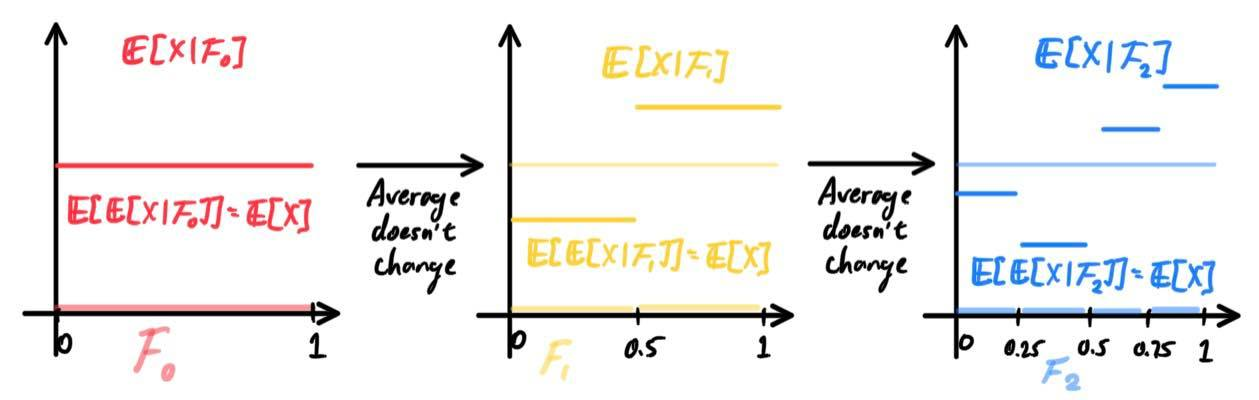
\includegraphics[scale=0.3]{img/martingale_increments.jpg}
  \end{center}
  
  A supermartingale (and submartingale) just means that as we make the function finer and finer, its mean goes down (or up). 


  Martingales are used to model lots of random walk events. In the following three examples, let $\xi_1, \xi_2, \ldots$ be iid, and let $S_n = S_0 + \xi_1 + \ldots + \xi_n$., where $S_0$ is a constant. Let $\mathcal{F}_n = \sigma(\xi_1, \ldots, \xi_n)$ for $n \geq 1$ and let $\mathcal{F}_0 = \{\emptyset, \Omega\}$. 

  \begin{example}[Linear Martingale]
    \label{ex:linear-martingale}
    Let $\mu = \mathbb{E}[\xi_i] = 0$. Then, $\{S_n\}$ is a martingale with respect to $\mathcal{F}_n$. We show the three requirements: 
    \begin{enumerate}
      \item $\mathbb{E}[S_n] = \mathbb{E}[S_0] + \mathbb{E}[\xi_1] + \ldots + \mathbb{E}[\xi_n] = S_0 < \infty$. 
      
      \item By definition, we know that $\xi_i$ is $\sigma(\xi)$-measurable for all $i \in [n]$, so $\xi_i$ is $\mathcal{F}_n = \sigma(\xi_1, \ldots, \xi_n)$-measurable. Since the set of $\mathcal{F}_n$-measurable functions has a \hyperref[lin-def:vector-space]{vector space} structure, $S_n$ is also $\mathcal{F}_n$-measurable. 
      
      \item We can simply solve 

        \begin{equation}
          \mathbb{E}[S_{n+1} \mid \mathcal{F}_n] = \mathbb{E}[S_n \mid \mathcal{F}_n] + \mathbb{E}[\xi_{n+1} \mid \mathcal{F}_n] = X_n + \mathbb{E}[\xi_{n+1}] = X_n
        \end{equation}

      where the first equality follows from linearity. For the second equality, note that $S_n$ is $\mathcal{F}_n$-measurable from above, and so the best $\mathcal{F}_n$-measurable approximation of $X$ is $X$ itself (i.e. we have complete information). We know that $\xi_{n+1}$ is independent of the $\xi_i$'s, and so by definition their $\sigma$-algebras are independent. This implies that $\sigma(\xi_{n+1})$ and $\mathcal{F}_n = \sigma(\xi_1, \ldots, \xi_n)$ are independent, and so due to irrelevant information, $\mathbb{E}[\xi_{n+1} \mid \mathcal{F}_n] = \mathbb{E}[\xi_{n+1}]$. 
    \end{enumerate}
    If $\mu \leq 0$ or $\mu \geq 0$, then the computation above shows that $\mathbb{E}[S_{n+1} \mid \mathcal{F}_n] \leq 0$ or $\mathbb{E}[S_{n+1} \mid \mathcal{F}_n] \geq 0$, making it a supermartingale or submartingale, respectively. 
  \end{example}

  Given a supermartingale or submartingale, we can change it to be a \hyperref[def:martingale]{martingale}. 

  \begin{example}[Centred Random Walk as a Martingale]
    \label{ex:centred-random-walk-as-a-martingale}
  Given that $\mu = \mathbb{E}[\xi_i] \neq 0$, then $\{S_n - n\mu\}$ is a martingale with respect to $\mathcal{F}_n$. We can see this because

  \begin{align*}
    \mathbb{E}[S_{n+1} - (n + 1)\mu \mid \mathcal{F}_n] & = \mathbb{E}[S_n - n \mu \mid \mathcal{F}_n] + \mathbb{E}[\xi_{n+1} - \mu \mid \mathcal{F}_n] \\
    & = S_n - n \mu + \mathbb{E}[\xi_{n+1}] - \mu \\
    & = S_n - n
  \end{align*}
  \end{example}

  \begin{example}[Quadratic Martingale]
    \label{ex:quadratic-martingale}
  Say $\mu = \mathbb{E}[\xi_i] = 0$ and $\sigma^2 = \mathrm{Var}(\xi_i) < \infty$. Then, $\{S_n^2 - n \sigma^2\}$ is a martingale. 

  \begin{align*}
    \mathbb{E}[S_{n+1}^2 - (n + 1) \sigma^2 \mid \mathcal{F}_n] & = \mathbb{E}[ (S_n + \xi_{n+1})^2 - (n _ 1) \sigma^2 \mid \mathcal{F}_n] \\
    & = \mathbb{E}[S^2 - n \sigma^2 \mid \mathcal{F}_n ] + \mathbb{E}[ 2 S_n \xi_{n+1} + \xi_{n+1}^2 - \sigma^2 \mid \mathcal{F}_n] \\
    & = \mathbb{E}[S^2 - n \sigma^2 \mid \mathcal{F}_n ] + 2 \mathbb{E}[ S_n \xi_{n+1} \mid \mathcal{F}_n ] + \mathbb{E}[\xi_{n+1}^2] - \sigma^2  \\
    & = \mathbb{E}[S^2 - n \sigma^2 \mid \mathcal{F}_n ]
  \end{align*}

  where we have used the fact that due to independence of $\xi_{n+1}$ with $\mathcal{F}_n$, we have $\mathbb{E}[S_n \xi_{n+1} \mid \mathcal{F}_n] = \mathbb{E}[S_n \mathbb{E}[ \xi_{n+1} \mid \mathcal{F}_n]] = \mathbb{E}[S_n \cdot 0] = 0$. 
  \end{example}

  This following result shows that \hyperref[def:martingale]{martingales} with bounded increments either converge or oscillate between $+\infty$ and $-\infty$. 

  \begin{theorem}[Martingale Convergence under Bounded Increments]
    \label{thm:martingale-convergence-under-bounded-increments}
    Let $\{X_n\}_{n \in \mathbb{N}}$ be a \hyperref[def:martingale]{martingale} with $|X_{n+1} - X_n| \leq M < \infty$. Let 

    \begin{align*}
      C & = \{\lim_{n \rightarrow \infty} X_n \text{ exists and is finite}\} \\
      D & = \{\lim_{n \rightarrow \infty} \sup X_n = +\infty \text{ and } \lim_{n \rightarrow \infty} \inf X_n = -\infty\}
    \end{align*}

    Then $\mathbb{P}(C \cup D) = 1$. 
  \end{theorem}

  Note that as you get more and more information, your $\sigma$-algebra can "grow" and get closer to something that models complete information. This means that given some $\sigma$-algebra $\mathcal{F}$ that models complete information, we can take a sequence of nondecreasing sub-$\sigma$-algebras of $\mathcal{F}$ 
  \begin{equation}
    \mathcal{F}_1 \subset \mathcal{F}_2 \subset \ldots \subset \mathcal{F}_i \subset \ldots
  \end{equation}
  such that $\mathcal{F}_i \subset \mathcal{F}$, which models our increasing knowledge of the experiment. 



  \begin{example}[Filtration of 3 Coin Tosses]
    \label{ex:filtration-of-3-coin-tosses}
    Let us describe a concrete example of a 3-coin toss filtration. The \hyperref[prob-def:probability-space]{probability space} is 
    \begin{equation}
      \Omega = \{000, 001, 010, 011, 100, 101, 110, 111\}
    \end{equation}
    which has $8$ outcomes so a complete $\sigma$-algebra would consist of $2^8 = 256$ outcomes. 
    \begin{enumerate}
      \item Before the experiment, we have no information at all, so 
      \begin{equation}
        \mathcal{F}_0 = \{\emptyset, \Omega\}
      \end{equation}
      which has $2^{2^0} = 2$ elements. 
      
      \item After the first coin toss, we would have information on what the first flip landed on (whether it was of form $( 0, \ast, \ast)$ or $(1, \ast, \ast)$), so we have a $\sigma$-algebra generated by these two events 
      \begin{align*}
        \mathcal{F}_1 & = \sigma(\{( 0, \ast, \ast)\}, \{(1, \ast, \ast)\}) \\
        & = \sigma(\{000, 001, 010, 011\}, \{100, 101, 110, 111\}) \\
        & = \{\emptyset, \{000, 001, 010, 011\}, \{100, 101, 110, 111\}, \Omega\}
      \end{align*}
      which has $2^{2^1} = 4$ elements. 
      
      \item After the second coin toss, we would have information on what the first two flips landed on (whether it was of form $( 0, 0, \ast)$, $( 0, 1, \ast)$, $(1, 0, \ast)$, $(1, 1, \ast)$), so we have a $\sigma$-algebra generated by these 4 events 
      \begin{align}
        \mathcal{F}_2 & = \sigma(\{( 0, 0, \ast)\}, \{( 0, 1, \ast)\}, \{(1, 0, \ast)\}, \{(1, 1, \ast)\}) \\
        & = \sigma(\{000, 001\}, \{010, 011\}, \{100, 101\}, \{110, 111\}) \\
        & = \{\emptyset, \{000, 001\}, \{010, 011\}, \{100, 101\}, \{110, 111\}, \\
        & \;\;\;\;\;\; \{000, 001, 010, 011\}, \{000, 001, 100, 101\}, \{000, 001, 110, 111\}, \\
        & \;\;\;\;\;\; \{010, 011, 100, 101\}, \{010, 011, 110, 111\}, \{100, 101, 110, 111\}, \\ 
        & \;\;\;\;\;\; \{000, 001, 010, 011, 100, 101\}, \{000, 001, 010, 011, 110, 111\}, \\
        & \;\;\;\;\;\; \{000, 001, 110, 101, 110, 111\}, \{010, 011, 110, 101, 110, 111\},  \Omega\}
      \end{align}
      which has $2^{2^2} = 16$ elements. 
      
      \item After the third coin toss, we would have information on what the first three flips landed on (all 8 possibilities in $\Omega$), so we have a $\sigma$-algebra generated by these 8 events 
      \begin{align}
        \mathcal{F}_3 & = \sigma(\{000\}, \{001\}, \{010\}, \{011\}, \{100\}, \{101\}, \{110\}, \{111\})
      \end{align}
      This is too big to write down explicitly, but it has $2^{2^3} = 256$ elements. 
    \end{enumerate}
  \end{example}


	Remember that for a \hyperref[prob-def:random-variable]{random variable} $X$ and $\sigma$-algebras $\mathscr{F}_1, \mathscr{F}_2$ s.t. $\mathscr{F}_1 \subset \mathscr{F}_2$, by the tower property, 
	\begin{equation}
		\mathbb{E}[ \mathbb{E}[X \mid \mathscr{F}_2] \mid \mathscr{F}_1] = \mathbb{E}[X \mid \mathscr{F}_1] 
	\end{equation}

	If we exchange the two, the smaller one wins. but for arbitrary $\sigma$-algebras, equality does not hold.\footnote{No direct connection to \hyperref[mt-thm:fubinis-theorem]{Fubini's theorem}.}
	\begin{equation}
		\mathbb{E}[ \mathbb{E}[X \mid \mathscr{F}_2] \mid \mathscr{F}_1] \neq \mathbb{E}[ \mathbb{E}[X \mid \mathscr{F}_1] \mid \mathscr{F}_2]
	\end{equation}

	It is useful to consider when $\mathscr{F}_2 \not\subset \mathscr{F}_1$ and $\mathscr{F}_1 \not\subset \mathscr{F}_2$. 

	\begin{example}[Filtrations on a Three-Point Space]
	  \label{ex:filtrations-on-a-three-point-space}
		The prototypical example is $\Omega = \{a, b, c\}$ with $\mathbb{P}(\{a\}) = \mathbb{P}(\{b\}) = \mathbb{P}(\{c\}) = \frac{1}{3}$. Then, $X(a) = 1, X(b) = 2, X(c) = 3$. Consider the following $\sigma$-algebras: 
		\begin{enumerate}
			\item $\mathscr{F}_1$ generated by $\{a, b\}, \{c\}$. 
			\item $\mathscr{F}_2$ generated by $\{a\}, \{b, c\}$. 
		\end{enumerate}
		Then, 
		\begin{align}
			\mathbb{E}[X \mid \mathscr{F}_1](\omega) & = \begin{cases} 
				1.5 & \text{ if } \omega \in \{a, b\} \\ 
				3 & \text{ if } \omega \in \{c\} 
			\end{cases} \implies \mathbb{E}[ \mathbb{E}[X \mid \mathscr{F}_1] \mid \mathscr{F}_2] = 
			\begin{cases} 
				1.5 & \text{ if } \omega \in \{a\} \\ 
				2.75 & \text{ if } \omega \in \{b, c\} 
			\end{cases} \\ 
			\mathbb{E}[X \mid \mathscr{F}_2](\omega) & = \begin{cases} 
				1 & \text{ if } \omega \in \{a\} \\ 
				2.5 & \text{ if } \omega \in \{b, c\} 
			\end{cases} \implies \mathbb{E}[ \mathbb{E}[X \mid \mathscr{F}_2] \mid \mathscr{F}_1] = 
			\begin{cases} 
				1.75 & \text{ if } \omega \in \{a, b\} \\ 
				2.5 & \text{ if } \omega \in \{c\} 
			\end{cases}
		\end{align}
	\end{example}

	

	\begin{definition}[Martingale]
	  \label{def:martingale}
	  If $X_n$ further satisfies 
		\begin{enumerate}
			\item $\mathbb{E}[|X_n|] < +\infty$ (so that we don't run into any problems in cord exp)
			\item $\mathbb{E}[X_n \mid \mathscr{F}_{n-1}] = X_{n-1}$. 
		\end{enumerate}
		Then $(X_n)$ is called a \textbf{martingale}. If instead of (2), we have 
		\begin{enumerate}
		  \item $\mathbb{E}[X_n \mid \mathscr{F}_{n-1}] \leq X_{n-1}$, then $(X_n)$ is a \textbf{supermartingale}. 
		  \item $\mathbb{E}[X_n \mid \mathscr{F}_{n-1}] \geq X_{n-1}$, then $(X_n)$ is a \textbf{submartingale}. 
		\end{enumerate}
	\end{definition}

	\begin{example}[Random Walk]
	  \label{ex:random-walk}
	  Let $Y_1, \ldots$ be iid \hyperref[prob-def:random-variable]{random variables} and define 
		\begin{equation}
			S_n = S_0 + \sum_{i=1}^n Y_i
		\end{equation}
		where $S_0$ is a constant. To specify a \hyperref[def:filtration]{filtration}, a canonical way of constructing it is to just let it be generated by the random variables. So, 
		\begin{equation}
			\mathscr{F}_0 = \{\empty,  \Omega\}, \qquad \mathscr{F}_n = \sigma(Y_1, \ldots, Y_n)
		\end{equation}
		For (1) to hold, just assume $\mathbb{E}[|Y_i|] < +\infty \implies \mathbb{E}[|S_n|] < +\infty$ by triangle inequality. So, by our construction, we get 
		\begin{equation}
			\mathbb{E}[S_n \mid \mathscr{F}_{n-1}] = \underbrace{S_0 + \sum_{i=1}^{n-1} Y_i}_{= S_{n-1}} + \underbrace{\mathbb{E}[Y_n \mid \mathscr{F}_{n-1}]}_{= \mathbb{E}[Y_n]} 
		\end{equation}
		where $\mathbb{E}[Y_n \mid \mathscr{F}_{n-1}] = \mathbb{E}[Y_n]$ since $Y_n$ is independent of $\mathscr{F}_{n-1}$. So, 
		\begin{enumerate}
			\item if $\mathbb{E}[Y_n] = 0$, $S_n$ is a \hyperref[def:martingale]{martingale}. 
			\item if $\mathbb{E}[Y_n] > 0$, $S_n$ is a submartingale. 
			\item if $\mathbb{E}[Y_n] < 0$, $S_n$ is a supermartingale. 
		\end{enumerate}
	\end{example}

	\begin{example}[Products of Nonnegative Random Variables]
	  \label{ex:products-of-nonnegative-random-variables}
	  Now let 
		\begin{equation}
			M_n = \prod_{i=1}^n Y_i, \qquad Y_i \geq 0
		\end{equation}
		and assume $\mathbb{E}[Y_i]^2 < +\infty$. Then, by \hyperref[prob-thm:cauchy-schwarz]{Cauchy-Schwarz}, $\mathbb{E}[|M_n|] < +\infty$. Then, 
		\begin{equation}
			\mathbb{E}[M_n \mid \mathscr{F}_{n-1}] = \bigg( \prod_{i=1}^n Y_i \bigg) \mathbb{E}[Y_n] = M_{n-1} \mathbb{E}[Y_n]
		\end{equation}
		So, 
		\begin{enumerate}
			\item if $\mathbb{E}[Y_n] = 1$, $S_n$ is a \hyperref[def:martingale]{martingale}. 
			\item if $\mathbb{E}[Y_n] > 1$, $S_n$ is a submartingale. 
			\item if $\mathbb{E}[Y_n] < 1$, $S_n$ is a supermartingale. 
		\end{enumerate}
	\end{example}

	Now for some abstract properties of \hyperref[def:martingale]{martingales}. 

	\begin{lemma}[Supermartingale Inequality over Several Steps]
	  \label{thm:supermartingale-inequality-over-several-steps}
 
		If $X_n$ is a supermartingale, then for all $n > m$, $\mathbb{E}[X_n \mid \mathscr{F}_m] \leq X_m$.
	\end{lemma}
	\begin{proof}
	  Induct on $n$ and tower property. 
		\begin{align}
			\mathbb{E}[X_n \mid \mathscr{F}_m] & = \mathbb{E}[\mathbb{E}[X_n \mid \mathscr{F}_{n-1}] \mid \mathscr{F}_m ] && \tag{Tower Property} \\ 
																				 & \leq \mathbb{E}[X_{n-1} \mid \mathscr{F}_m ] && \tag{By Definition} \\ 
																				 & \leq X_m && \tag{Inductive Hypothesis}
		\end{align}
	\end{proof}

	\begin{corollary}[Multi-Step Submartingale and Martingale Identities]
	  \label{thm:multi-step-submartingale-and-martingale}
	  Let $X_n$ be adapted to the filtration $\mathscr{F}_n$. Then the following hold. 
		\begin{enumerate}
			\item If $X_n$ is a submartingale, then for all $n > m$, $\mathbb{E}[X_n \mid \mathscr{F}_m] \geq X_m$. 
			\item If $X_n$ is a  \hyperref[def:martingale]{martingale}, then for all $n > m$, $\mathbb{E}[X_n \mid \mathscr{F}_m] = X_m$. 
		\end{enumerate}
	\end{corollary}
	\begin{proof}
		We use the common ``symmetry trick.''
		\begin{enumerate}
		  \item $-X_n$ is a supermartingale and use the lemma. 
			\item $X_n$ is both a supermartingale and submartingale. 
		\end{enumerate}
	\end{proof}

	\begin{definition}[Predictable Sequence]
	  \label{def:predictable-sequence}
		For a \hyperref[def:filtration]{filtration} $(\mathscr{F}_n)_{n=0}^\infty$, a sequence of \hyperref[prob-def:random-variable]{random variables} $(H_n)_{n=1}^\infty$ is a \textbf{predictable sequence} if $H_n$ is measurable with respect to $\mathscr{F}_{n-1}$. 
	\end{definition}

	It is immediate that \hyperref[def:predictable-sequence]{predictable sequences} are adapted, since the $\sigma$-algebras are increasing in a \hyperref[def:filtration]{filtration}, i.e. $H_n$ is $\mathscr{F}_{n-1}$-measurable which implies $H_n$ is $\mathscr{F}_n$ measurable. Adapated sequences are not necessarily predictable. 

	\begin{example}[Gambling]
	  \label{ex:gambling}
	  At each round $r$, you bet \$x. With probability $p$, you win an additional \$x and with probability $1-p$, you lose \$x. Let 
		\begin{enumerate}
		  \item $X_n = $ not winning after $n$ rounds, if you bet \$1 each time. 
			\item $H_n = $ amount of money you bet in round $n+1$. So, makes sense to be $\mathscr{F}_{n+1}$-measurable. So, this is an example of a \hyperref[def:predictable-sequence]{predictable sequence}. 
			\item Now, our net earnings after $n$ rounds of the game is 
				\begin{equation}
					(H \cdot X)_n = \sum_{m=1}^n H_m (X_m - X_{m-1})
				\end{equation}
				where $X_m - X_{m-1} \in \{\pm 1\}$. 
		\end{enumerate}
		Now the strategy might be to double down if you lose, and keep betting \$1 if you win, so 
		\begin{equation}
			H_n = \begin{cases} 
				2 H_{n-1} & \text{ if } X_{n-1} - X_{n-2} = -1 \\ 
				1 & \text{ if } X_{n-1} - X_{n-2} = \pm 1
			\end{cases} 
		\end{equation}
		This betting strategy is called a \hyperref[def:martingale]{martingale}. Remember that if we had infinite money, we will always win. More generally, if $(H \cdot X)_n$ is a submartingale, then $\mathbb{E}[(H \cdot X)_n] \geq 0$. So, we should consider cases which leads to $(H \cdot X)_n$ being a submartingale. 
	\end{example}

	\begin{theorem}[Discrete Stochastic Integral of a Supermartingale]
	  \label{thm:discrete-stochastic-integral-of-a}
		Let $X_n$, $n \geq 0$ be a supermartingale. If $H_n \geq 0$ is predictable and each $H_n$ is bounded (pointwise), then $(H \cdot X)_n$ is a super-martingale. 
	\end{theorem}
	\begin{proof}
	  We have 
		\begin{align}
			\mathbb{E}[(H \cdot X)_{n+1} \mid \mathscr{F}_n] & = (H \cdot X)_n + \mathbb{E}[H_{n+1} (X_{n+1} - X_n) \mid \mathscr{F}_n ] \\ 
																											 & = (H \cdot X)_n + H_{n+1} \mathbb{E}[\underbrace{X_{n+1} - X_n}_{\leq 0} \mid \mathscr{F}_n ] \\ &
																											& \leq (H \cdot X)_n 
		\end{align}
	\end{proof}


	\begin{theorem}[Stopped Supermartingales]
	  \label{thm:stopped-supermartingales}
		If $N$ is a \hyperref[def:stopping-time]{stopping time}, and $X_n$ is a supermartingale, then $X_{N \wedge n}$ (where $N \wedge n$) is a supermartingale. This is a stopped version. 
	\end{theorem}
	\begin{proof}
	  We can write 
		\begin{equation}
			X_{N \cap n} = \bigg( \sum_{m=1}^n H_m (X_m - X_{m-1}) \bigg) + X_0
		\end{equation}
		where $H_m = \mathbbm{1}(N \geq m)$. Check that it is predictable, and then conclude by theorem 1. 
	\end{proof}

	\begin{example}[Upcrossing Times of a Submartingale]
	  \label{ex:upcrossing-times-of-a-submartingale}
		Suppose $(X_n)_{n \geq 0}$ is a submartingale. Let $a < b$, $N_0 = -1$. For $k \geq 1$, let 
		\begin{enumerate}
			\item $N_{2k-1} = \inf\{m > N_{2k-2} \colon X_m \leq a \}$, i.e. when are you going below $a$? 
			\item $N_{2k} = \inf \{m > N_{2k-1} \colon X_m \geq b \}$ , i.e. when are you going above $b$? 
		\end{enumerate}
		We claim that $N_j$ are \hyperref[def:stopping-time]{stopping times}. We call $U_n = \sup \{k \colon N_{2k} \leq n\}$ as the number of upcrossings completed by time $n$. Next, we have the upcrossing inequality, which is used the prove the \hyperref[def:martingale]{martingale} convergence theorem.  
	\end{example}

	\begin{theorem}[Upcrossing Inequality]
	  \label{thm:upcrossing-inequality}
		If $(X_m)_{m \geq 0}$ is a submartingale, then 
		\begin{equation}
			(b - a) \mathbb{E}[U_n] \leq \mathbb{E}[(X_n - a)^+] - \mathbb{E}[(X_0 - a)^+]
		\end{equation}
	\end{theorem}

	The \hyperref[def:martingale]{martingale} convergence theorem is like an analogous version of the Bolzano-Weierstrass theorem---that a \hyperref[st-def:monotone-sequence]{monotone sequence} bounded above converges.

\section{Brownian Motion}


\subsection{Stochastic Matrices}

  \begin{definition}[Entrywise Positive]
    A real $n \times n$ matrix $P$ is \textbf{entrywise positive} if all entries are positive real numbers. We similarly define entrywise positive vectors having components as positive real numbers. With this notion of positiveness. We can define
    \begin{equation}
      A > B \iff A - B > 0 \iff (A-B)_{i j} > 0 \; \forall i, j
    \end{equation}
  \end{definition}

  Note that this definition of positive matrices is \textit{not} the same as positive-definite matrices! 

  \begin{theorem}[Perron's Theorem]
    Every entrywise positive matrix $P$ has a real \textbf{dominant eigenvalue}, denoted $\lambda(P) \in \mathbb{R}$ satisfying
    \begin{enumerate}
      \item $\lambda(P) > 0$, and the associated eigenvector $h >0$
      \item $\lambda(P)$ is a simple eigenvalue
      \item every other eigenvalue $\kappa$ satisfies: $|\kappa| < \lambda(P)$
      \item there is no other eigenvector $\geq 0$, i.e. all other eigenvectors have at least 1 negative entry.
    \end{enumerate}
  \end{theorem}

  \begin{definition}[Stochastic Matrix]
    A \textbf{stochastic matrix} is a matrix $A$ where the elements of each column $a_i$ sum up to $1$. $A$ is \textbf{doubly stochastic} if $A$ and $A^T$ are stochastic. 
  \end{definition}

  \begin{theorem}[Spectral Radius of a Positive Stochastic Matrix]
    Let $S > 0$ be a positive stochastic matrix. Then, $\lambda(S) = 1$. Furthermore, given any nonnegative vector $x \geq 0$, 
    \begin{equation}
      \lim_{N \rightarrow \infty} S^N x = c h
    \end{equation}
    where $h$ is the dominant eigenvector and $c$ is some positive constant. 
  \end{theorem}

  A common application of this theorem likes in probability and statistics. Since nonnegative stochastic matrices can be used to represent discrete-time Markov Chains, with the dominant eigenvector representing the stationary distribution $\pi$. 

  Another application lies within defining Google's Page Rank Algorithm. Upon representing a page as a node, if there is one link that directs the user from page $A$ to page $B$, we can represent this as an oriented path from node $A$ to node $B$. Given that we have $n$ nodes, we can construct a $n \times n$ matrix $A$ where 
  \begin{equation}
    a_{i j} \coloneqq  \frac{\text{number of paths from node $i$ to node $j$}}{\text{number of nonzero entries in $j$th column}}
  \end{equation}

  \begin{figure}[H]
    \centering
    \begin{subfigure}[b]{0.48\textwidth}
      \centering
      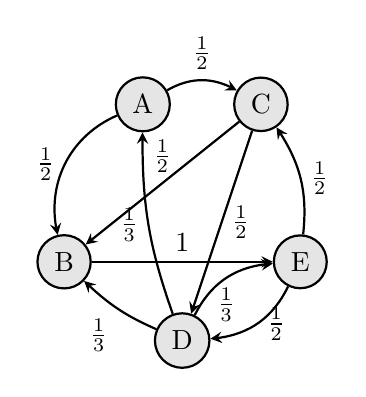
\begin{tikzpicture}[
        scale=0.5,
        ->,
        >=stealth,
        node distance=4cm,
        thick,
        main node/.style={circle, draw, fill=black!10, minimum size=4mm}
        ]

        % Nodes/States
        \node[main node] (A) at (0,4) {A};
        \node[main node] (B) at (-2,0) {B};
        \node[main node] (C) at (3,4) {C};
        \node[main node] (D) at (1,-2) {D};
        \node[main node] (E) at (4,0) {E};

        % Edges with reversed direction
        % From A to B (curving outwards)
        \path (A) edge [bend right=40] node[left] {$\frac{1}{2}$} (B);
        \path (A) edge [bend left=30] node[above] {$\frac{1}{2}$} (C);
        
        % From B to other states
        \path (C) edge node[above] {$\frac{1}{2}$} (B);
        \path (D) edge [bend left=10] node[below left] {$\frac{1}{3}$} (B);
        \path (D) edge [bend left=10] node[left] {$\frac{1}{3}$} (A);
        
        % From E to C (corrected direction)
        \path (E) edge [bend right=20] node[right] {$\frac{1}{2}$} (C);
        
        % From D to other states
        \path (C) edge  node[right] {$\frac{1}{2}$} (D);
        \path (D) edge [bend left=30] node[below] {$\frac{1}{3}$} (E);
        
        % From E to other states
        \path (B) edge node[above] {$1$} (E);
        \path (E) edge [bend left=30] node[right] {$\frac{1}{2}$} (D);
      \end{tikzpicture}
    \end{subfigure}
    \hfill 
    \begin{subfigure}[b]{0.48\textwidth}
      \centering
      \begin{equation}
        \begin{pmatrix}0&0&0&\frac{1}{3}&0\\
        \frac{1}{2}&0&\frac{1}{2}&\frac{1}{3}&0\\
        \frac{1}{2}&0&0&0&\frac{1}{2}\\
        0&0&\frac{1}{2}&0&\frac{1}{2}\\
        0&1&0&\frac{1}{3}&0\end{pmatrix}
      \end{equation}
    \end{subfigure}
    \caption{Markov chain graph and corresponding adjacency/transition matrix.}
    \label{fig:markov_chain}
  \end{figure}

  However, the theorem above requires the matrix to be strictly positive, which is often not true for Markov chains in general. This theorem does not hold true in the following example, 
  \begin{equation}
    A = \begin{pmatrix}
    0&0&0&\frac{1}{3} \\
    \frac{1}{2}&0&0&\frac{1}{3} \\
    0&0&0&\frac{1}{3} \\
    \frac{1}{2}&0&0&0
    \end{pmatrix} \implies A^{1000} 
        \begin{pmatrix}
    \frac{1}{4} \\ \frac{1}{4} \\ \frac{1}{4} \\ \frac{1}{4}
    \end{pmatrix} = 
        \begin{pmatrix}
    0 \\ 9/20 \\ 11/20 \\ 0
    \end{pmatrix}, \; A^{1001} 
        \begin{pmatrix}
    \frac{1}{4} \\ \frac{1}{4} \\\frac{1}{4} \\ \frac{1}{4}
    \end{pmatrix} = 
        \begin{pmatrix}
    0 \\ 11/20 \\ 9/20 \\ 0
    \end{pmatrix}
  \end{equation}
  That is, $A^N v$ oscillates between these two values. Furthermore, given three notes $A, B, C$ as such

  \begin{figure}[H]
    \centering 
    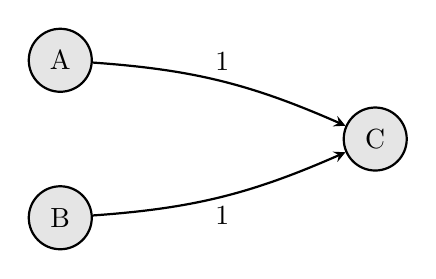
\begin{tikzpicture}[
      ->,
      >=stealth,
      node distance=3cm,
      thick,
      main node/.style={circle, draw, fill=black!10, minimum size=8mm}
      ]
      % Nodes
      \node[main node] (A) at (0,2) {A};
      \node[main node] (B) at (0,0) {B};
      \node[main node] (C) at (4,1) {C};

      % Edges with weight labels
      \path (A) edge [bend left=10] node[above] {$1$} (C);
      \path (B) edge [bend right=10] node[below] {$1$} (C);
    \end{tikzpicture}
    \label{fig:degenerate_markov_chain}
  \end{figure}
  the entries of the adjacency matrix is not well-defined. 
  \begin{equation}
     \begin{pmatrix} 0&0&? \\0&0&? \\1&1&?\end{pmatrix}
  \end{equation}
  Google CEO Larry Page actually developed a solution by implementing what he called a \textit{dampening factor}. Given stochastic matrix $B_{i j} = \frac{1}{N}$, he redefined the chain to be 
  \begin{equation}
    M = \alpha A + (1-\alpha) B, \; 0< \alpha < 1
  \end{equation}
  It is clear that $M$ is now a strictly positive stochastic matrix. The $\alpha$ is the dampening factor, and its optimal value is known to be about $0.67$. The value of the alpha determines how much of the data is "washed away." When $\alpha = 0$, none of the data is lost, and when $\alpha = 1$, all of the data is lost. 

  Due to the limitations of Perron's theorem, we can extend it with the following.

  \begin{theorem}[Frobenius Extension to Perron]
    Any $n \times n$ matrix $F \geq 0$, $F \neq 0$ has eigenvalue $\lambda$ such that
    \begin{enumerate}
      \item $\lambda \geq 0$ and $F h = \lambda h$, $h\geq 0$ \item every eigenvalue $\kappa$ satisfies: $|\kappa| \leq \lambda$ 
      \item if $|\kappa| = \lambda$, then 
      \begin{equation}
        \kappa = e^{\frac{2 \pi i k}{m}} \lambda, \; k, m \in \mathbb{Z}_+, \; m \leq n
      \end{equation}
    \end{enumerate}
  \end{theorem}


\end{document}
